\section{Introduzione}\label{introduzione}

\section{Normative}\label{normative}

In azienda la sicurezza informatica è strutturata a piramide, si parte
dal livello più in basso, il numero 4. Molto spesso le aziende
preferiscono partire dal primo livello che contiene le normative e le
regole senza però sapere qual'è il livello di conoscenza aziendale
sull\textquotesingle argomento informatico.

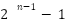
\includegraphics[width=6.26772in,height=2.51389in]{media/image10.png}

Esistono diverse caratteristiche che bisogna seguire per creare le nuove
normative, e sono:

\begin{itemize}
\item
  \textbf{Proporzionalità} \emph{{[}+ IMPORTANTE{]}}: la sicurezza non
  deve mai essere non sostenibile da una azienda;
\item
  \textbf{Prevenzione}: le norme devono prevenire gli incidenti e
  cercare di arrivare preparati in caso di attacco sapendo già le azioni
  da fare;
\item
  \textbf{Condivisione}: cioè riuscire a condividere con tutti le
  metodologie di attacchi e come proteggersi;
\item
  \textbf{Uniformità}: far sì che le normative siano applicabili fra
  loro e che tutte siano consone fra loro.
\end{itemize}

\subsection{GDPR}\label{gdpr}

Regolamentazione europea nata per tutelare gli utenti finali e i loro
dati, tutte le aziende che operano in territorio europeo (anche con sede
all'estero) devono sottostare al GDPR.

Il GDPR si applica ai dati personali di cittadini europei che vengono
trattati in maniera interamente o parzialmente automatizzata.

I dati coinvolti sono:

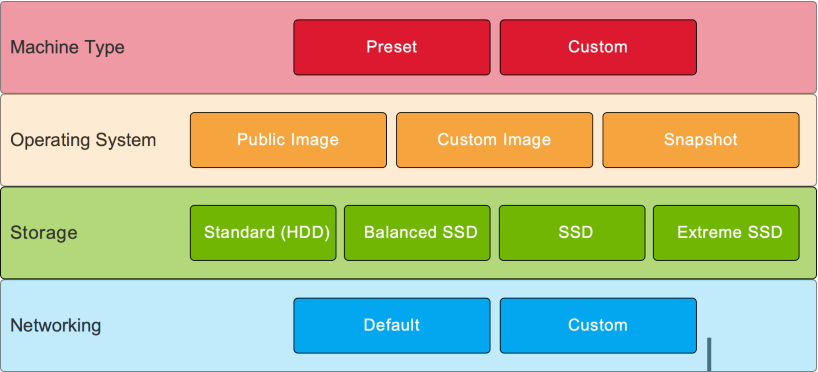
\includegraphics[width=6.26772in,height=3.47222in]{media/image37.png}

Nel GDPR si evidenziano anche alcuni attori:

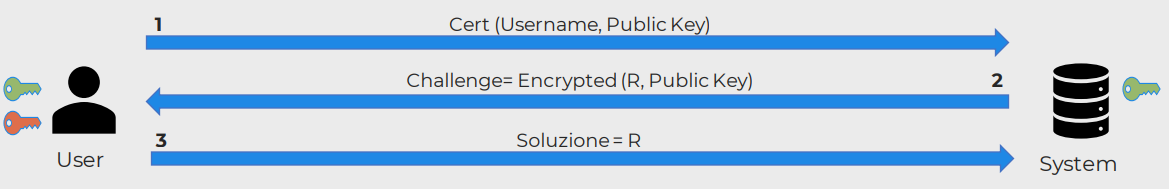
\includegraphics[width=6.26772in,height=3.11111in]{media/image111.png}

I diritti dell'interessato:

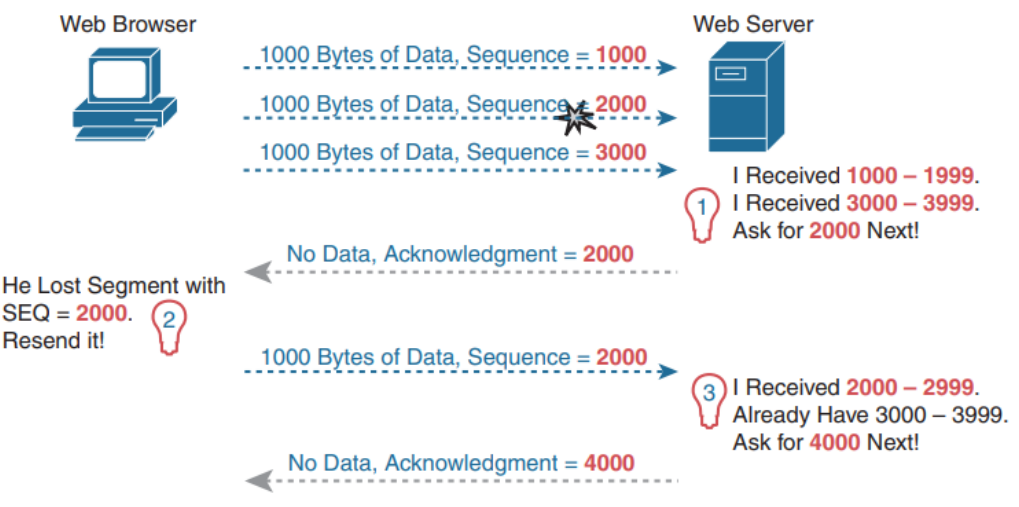
\includegraphics[width=6.26772in,height=2.95833in]{media/image75.png}

Il diritto di portabilità dice che per esempio una banca quando chiudete
il conto per farlo in un'altra è obbligata a fare il passaggio dei dati
per voi.

Il GDPR non impone normative tecniche precise ma è abbastanza generico e
astratto, ma impone misure di sicurezza per non cadere in sanzioni:

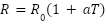
\includegraphics[width=6.26772in,height=2.44444in]{media/image43.png}

alcune soluzioni reali invece per proteggere i dati sono:

\begin{itemize}
\item
  \textbf{Anonimizzazione};
\item
  \textbf{Separazione};
\item
  \textbf{Conservazione cifrata e separata;}
\item
  \textbf{Cancellazione sicura e che avviene appena non più necessari};
\item
  \textbf{Cifratura sia a riposo che quando trasmetti};
\item
  \textbf{Applicare il principio del need-to-know};
\item
  \textbf{Definire strategie di risposta agli incidenti e di prevenzione
  e gestione del rischio a livello aziendale};
\item
  \textbf{Richiedere e mantenere il minimo dei dati strettamente
  necessari}.
\end{itemize}

In caso non si rispettino le soluzioni riportate sopra si può intaccare
in un data breach, un data breach consiste in un evento per il quale si
può compromettere la riservatezza, l\textquotesingle integrità e la
disponibilità dei dati a perimetro.

Questa casistica può avvenire tramite alcuni di questi attacchi:

\begin{itemize}
\item
  \textbf{comunicazione via email};
\item
  \textbf{comunicazione fisica/di persona};
\item
  \textbf{attacchi informatici fisici}.
\end{itemize}

In caso di attacchi il Titolare e/o il Responsabile sono tenuti a
notificarne l\textquotesingle avvenimento alle autorità entro 72 ore
tramite \emph{lesson learning} che riporta:

\begin{itemize}
\item
  la natura della violazione
\item
  nome e i dati di contatto del DPO
\item
  probabili conseguenze
\item
  misure adottate
\end{itemize}

ma va anche documentato ogni violazione ai dati personali e tenere
traccia delle comunicazioni tra le due figure.

Il GDPR indica anche le varie responsabilità, infatti il testo dice:

\emph{Chiunque subisca un danno materiale o immateriale causato da una
violazione del presente regolamento ha il diritto di ottenere un
risarcimento del danno dal \textbf{titolare del trattamento} o dal
\textbf{responsabile del trattamento}.}

Il \textbf{titolare} coinvolto risponde per il danno cagionato dalle sua
azioni che violano il GDPR.

Se il \textbf{responsabile} non rispetta volutamente le indicazioni del
titolare sarà lui a rispondere al risarcimento.

\subsection{PCI}\label{pci}

L'ente che ha redatto i vari standard è il PCI Council, opera a livello
globale a cui partecipano tutte le società che si occupano di pagamenti.

Va detto che in america è obbligatorio seguire le norme del PCI, in
europa no anche se fortemente consigliato visto che tutte le aziende che
non lo fanno probabilmente non riusciranno a stringere patti con altri
enti.

\emph{Il suo scopo è guidare l'adozione di standard uniformi al livello
di sicurezza riguardo le informazioni e fornendo risorse per la messa in
sicurezza dell'ecosistema dei pagamenti.}

I compiti principali sono:

\begin{itemize}
\item
  Definire standard di sicurezza per i pagamenti a livello globale
\item
  Validare e elencare prodotti e soluzioni che sono conformi con gli
  standard PCI (es. PCI SSC) e i relativi requisiti
\item
  Qualificare organizzazioni
\item
  Fornire un insieme di best practice per la sicurezza dei pagamenti
\end{itemize}

Gli standard rilasciati dal PCI Council sono 7 e sono:

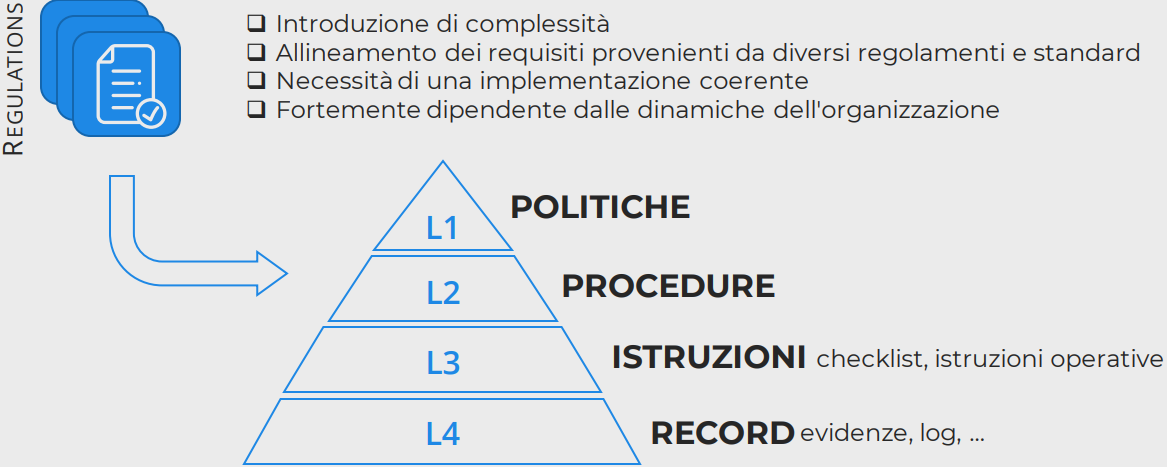
\includegraphics[width=6.26772in,height=1.93056in]{media/image18.png}

Sono presenti 8 principali ruoli definiti da PCI:

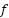
\includegraphics[width=6.85732in,height=2.68825in]{media/image44.png}

Ora possiamo vedere come i vari ruoli sono collocati nel processo di
pagamento:

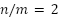
\includegraphics[width=6.88444in,height=1.36088in]{media/image120.png}

il card network cambia in base alla carta.

Per aderire al PCI è necessario attuare un processo continuo di
compliance e di sicurezza, strutturato secondo le seguenti fasi:

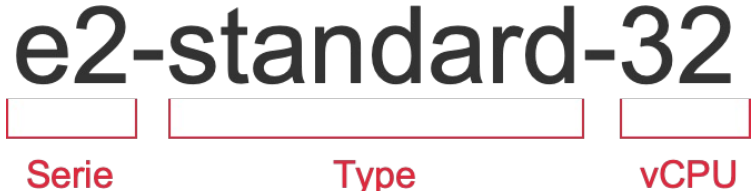
\includegraphics[width=6.26772in,height=1.625in]{media/image33.png}

I dati coinvolti dallo standard PCI sono detti account data, e sono
divisi fra cardholder data e sensitive authentication data:

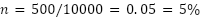
\includegraphics[width=6.26772in,height=3.47222in]{media/image113.png}

\subsubsection{PCI SSF}\label{pci-ssf}

Il PCI SSF (Secure Software Framework) è uno standard PCI che norma lo
sviluppo del software in maniera sicura. È composto da due parti, ognuna
delle quali si occupa di differenti aspetti applicativi:

\begin{itemize}
\item
  PCI Secure Software
\item
  PCI Secure Software Lifecycle
\end{itemize}

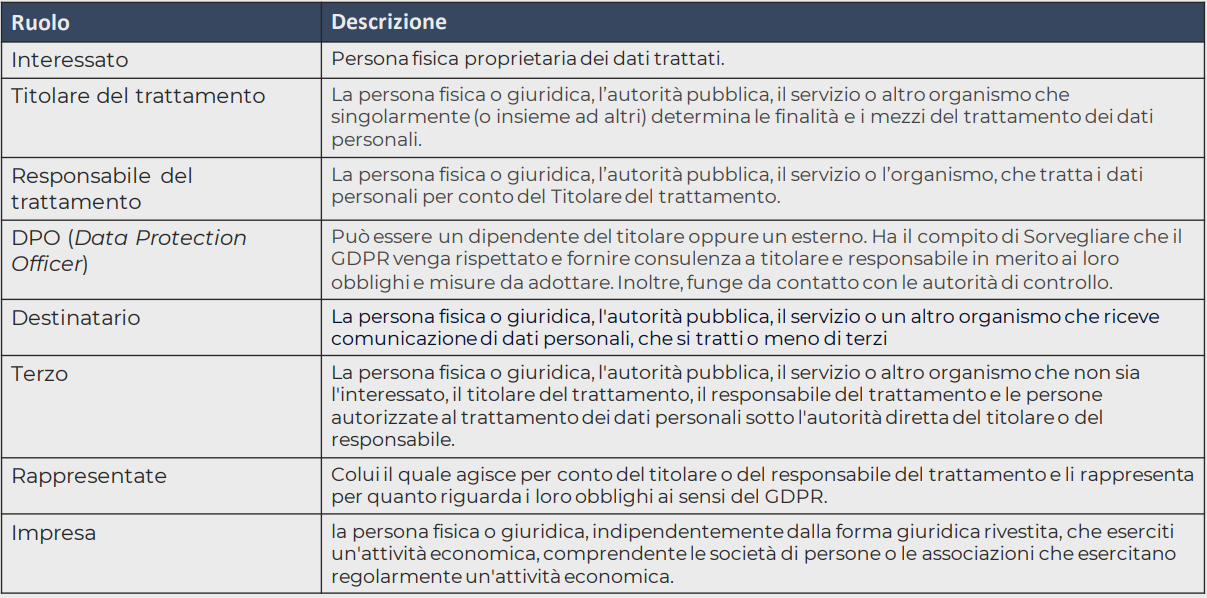
\includegraphics[width=4.49635in,height=2.73456in]{media/image110.png}

Seguendo il PCI SFF ti permettere di creare un secure payment software:

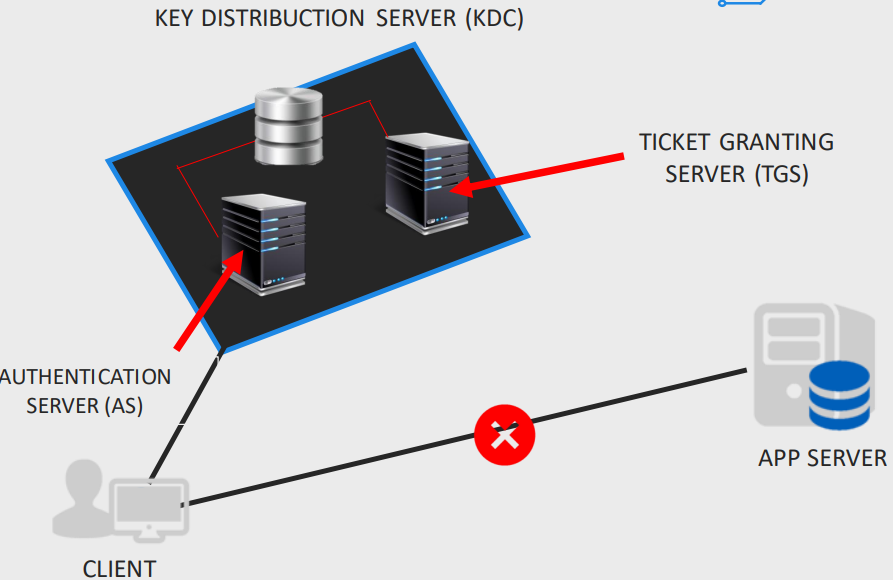
\includegraphics[width=6.26772in,height=2.5in]{media/image61.png}

\subsubsection{PCI DSS}\label{pci-dss}

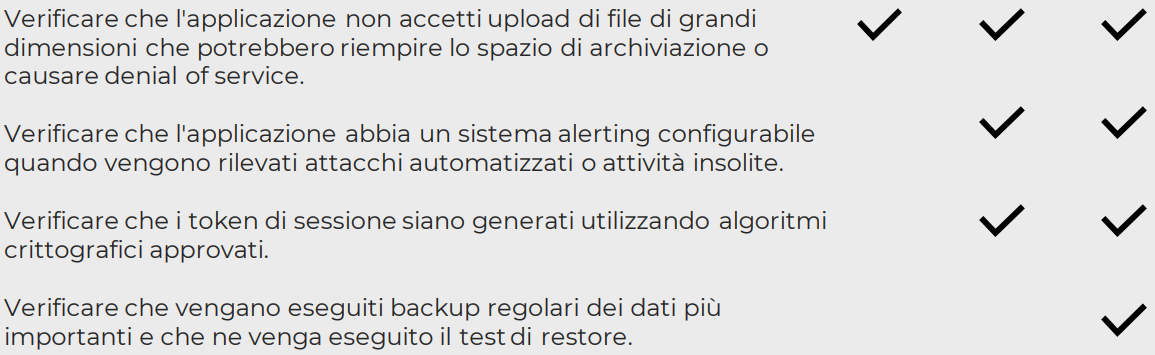
\includegraphics[width=6.90104in,height=3.40467in]{media/image83.png}

Figure che il PCI DSS controlla:

\begin{itemize}
\item
  Coloro che lavorano sui dati
\item
  Coloro che non usano direttamente i dati ma ne hanno accesso
\item
  Coloro che potrebbero mettere a rischio i dati anche se fuori dal loro
  ambiente
\end{itemize}

Lo standard PCI DSS migliora la sicurezza dei dati delle carte di
pagamento attraverso misure come la protezione dei dati dei titolari di
carta, il controllo degli accessi, il monitoraggio e il test delle reti,
e la gestione delle vulnerabilità. Queste misure aiutano le
organizzazioni a proteggere le informazioni sensibili da accessi non
autorizzati e frodi.

\subsection{Standard ISO}\label{standard-iso}

ISO è un\textquotesingle organizzazione internazionale indipendente che
sviluppa e pubblica standard tecnici per prodotti, servizi e sistemi a
livello globale, al fine di garantire la qualità,
l\textquotesingle efficienza e la sicurezza; contribuendo a creare un
ambiente di fiducia e cooperazione facilitando il commercio.

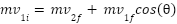
\includegraphics[width=6.26772in,height=2.20833in]{media/image35.png}

Una norma ISO è un documento tecnico che stabilisce: requisiti, linee
guida o specifiche per garantire la qualità,
l\textquotesingle affidabilità e la sicurezza di prodotti, servizi o
sistemi a livello internazionale.

Ogni norma è così strutturata: \textbf{ISO 9001:2015} dove ogni elemento
è:

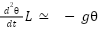
\includegraphics[width=6.80471in,height=0.99471in]{media/image31.png}

Le norme ISO sono cruciali nel commercio internazionale, poiché fungono
da linguaggio tecnico universale che supera barriere linguistiche e
culturali; agendo come un "passaporto commerciale" che semplifica gli
scambi internazionali.

In sintesi, le norme ISO contribuiscono a creare un ambiente di fiducia
e cooperazione benefico per la comunità globale degli affari.

Per garantire che le norma ISO vengano rispettate esistono due tipi di
audit:

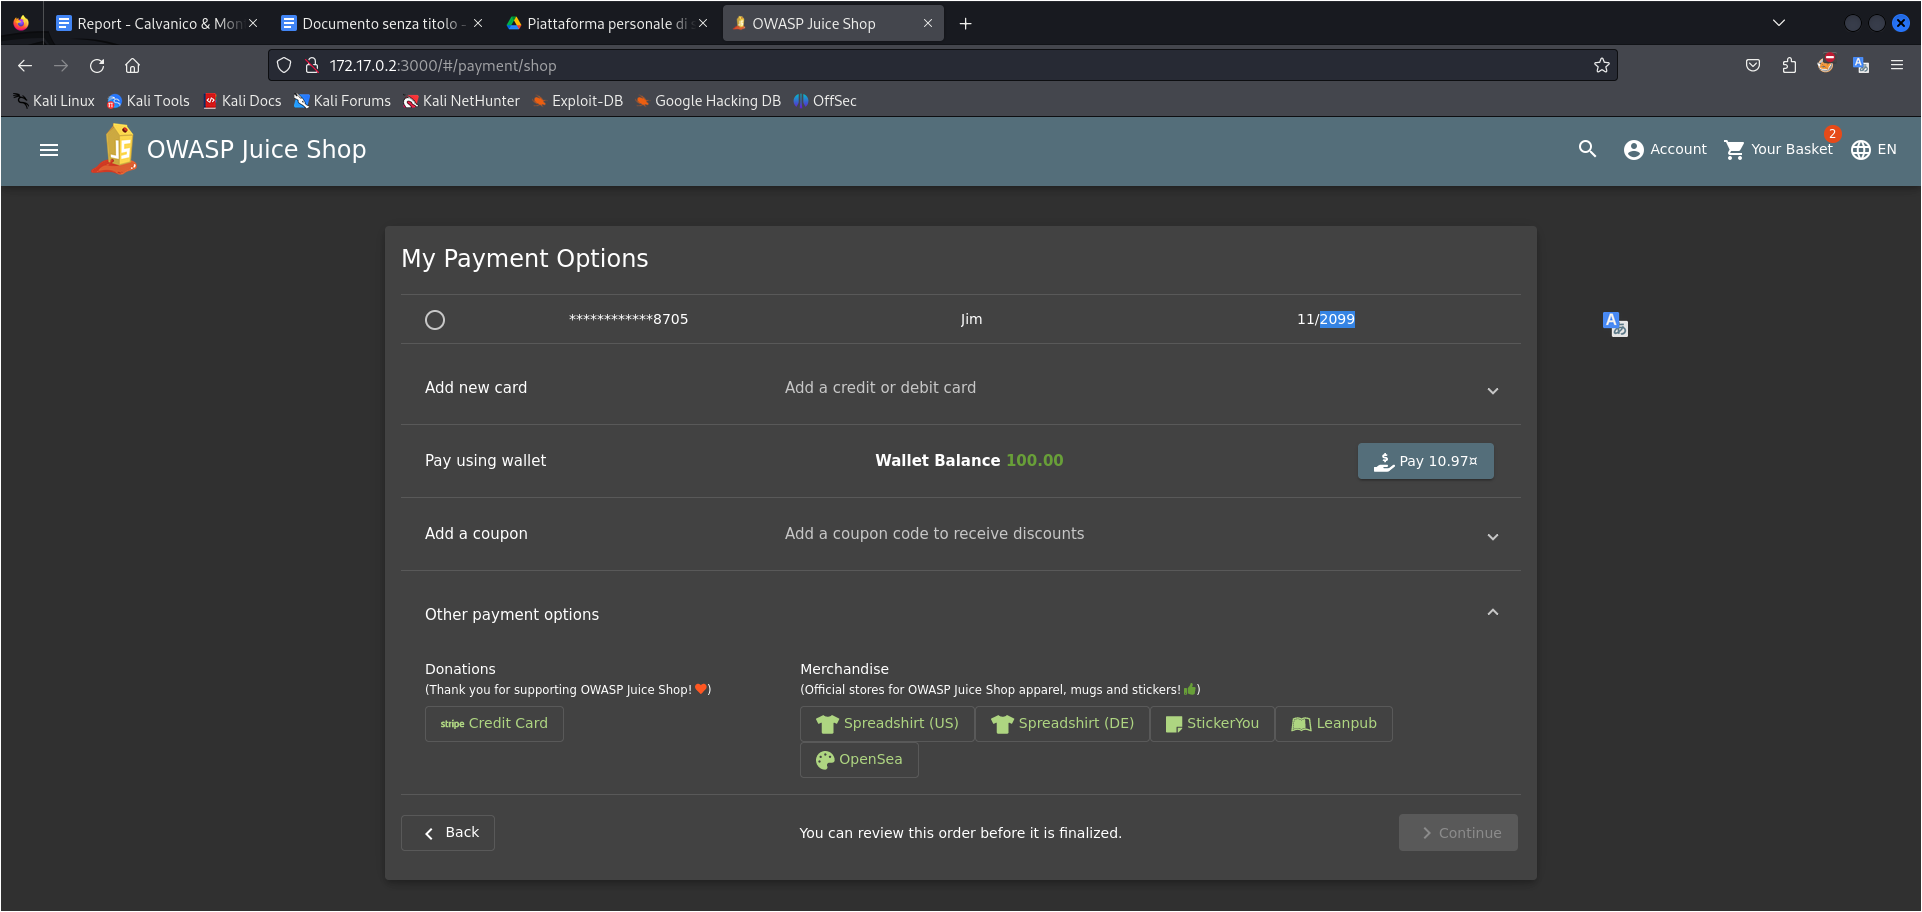
\includegraphics[width=2.19948in,height=2.59477in]{media/image12.png}

Quello interno viene fatto in maniera autonoma per prepararsi a quello
esterno (come una simulazione d'esame) per poi passare a quello esterno
dove viene in azienda una figura incaricata dalla ISO. Se l'auditor alla
fine del controllo pensa che tutto sia in regola rilascia una
certificazione.

Vediamo cos'è la certificazione:

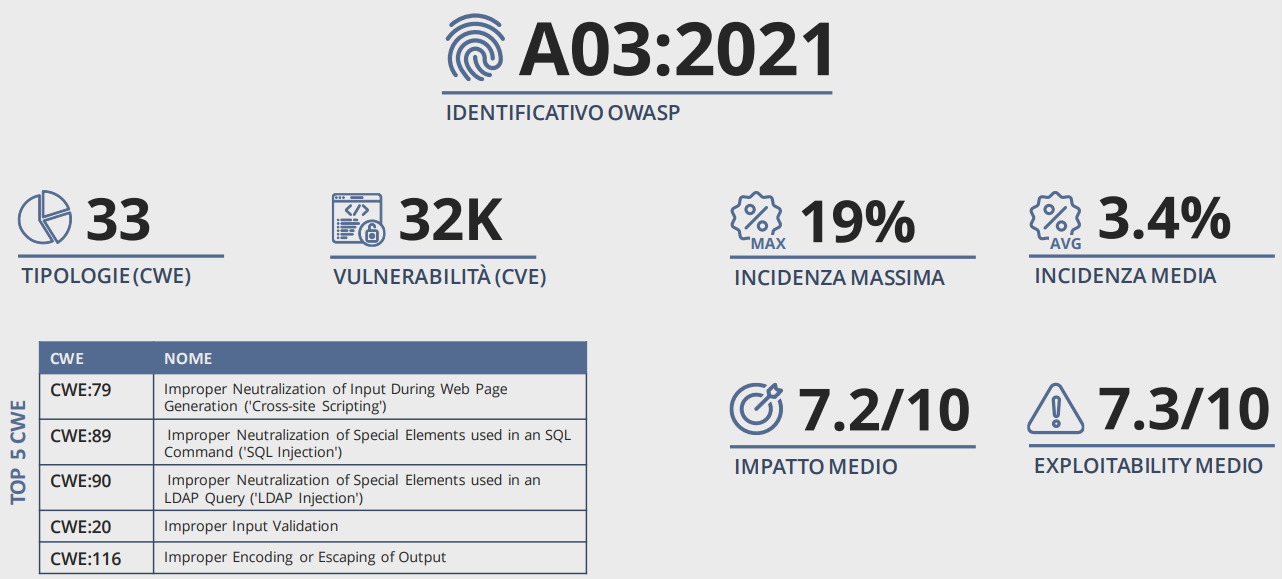
\includegraphics[width=3.45313in,height=1.81435in]{media/image89.png}

Ora vediamo alcune certificazioni ISO:

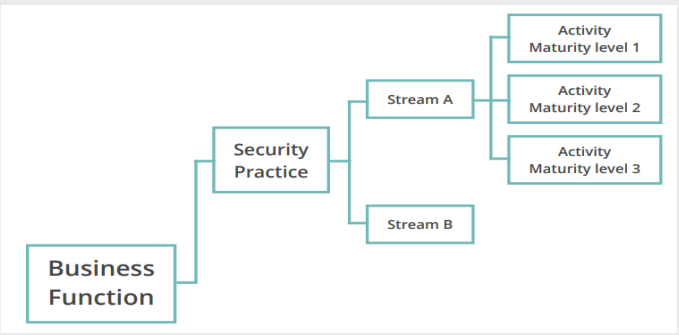
\includegraphics[width=6.26772in,height=2.97222in]{media/image96.png}

Tutti questi standard fanno parte della famiglia degli ISO 27000 che
rappresenta un insieme di norme internazionali focalizzate sulla
sicurezza delle informazioni. Essa fornisce un quadro strategico e
operativo per sviluppare, implementare, monitorare e migliorare
continuamente i processi di gestione della sicurezza delle informazioni
all\textquotesingle interno di un\textquotesingle organizzazione.

\emph{La famiglia ISO 27000 si concentra sul proteggere le informazioni
da minacce interne ed esterne, fornendo un approccio strutturato e
basato su best practice.}

Un'altra norma è la ISO 22301, dedicata al Business Continuity
Management (BCM), processo strategico che mira a identificare,
comprendere e mitigare i rischi che potrebbero minacciare la continuità
delle operazioni di un\textquotesingle organizzazione.

Per implementare la norma bisogna seguire principi fondamentali:

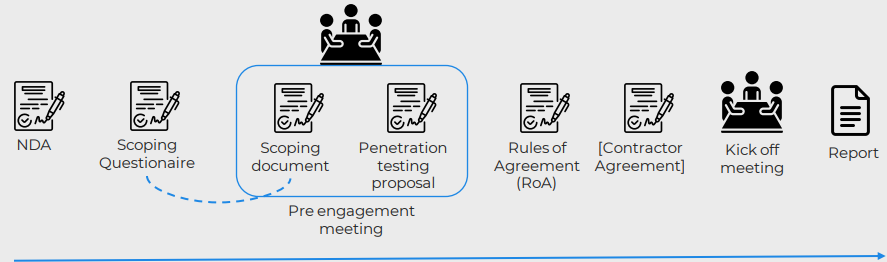
\includegraphics[width=6.26772in,height=3.08333in]{media/image58.png}

Nel dettaglio la creazione di BCP è un processo essenziale per garantire
che un\textquotesingle organizzazione possa mantenere operativi i suoi
processi critici in situazioni di emergenza o crisi.

\subsection{NIS2}\label{nis2}

Direttiva europea che aggiorna e amplia le misure di sicurezza per le
reti e i sistemi informativi degli operatori di servizi essenziali e dei
fornitori di servizi digitali, introducendo requisiti più rigorosi per
la gestione del rischio e la cooperazione tra gli Stati membri.

Tra le principali novità proposte sono presenti:

\begin{itemize}
\item
  l\textquotesingle estensione del campo di applicazione a nuovi
  settori, come l\textquotesingle energia, i trasporti e la sanità
\item
  l\textquotesingle introduzione di obblighi aggiuntivi per gli
  operatori di servizi essenziali e i fornitori di servizi digitali.
\end{itemize}

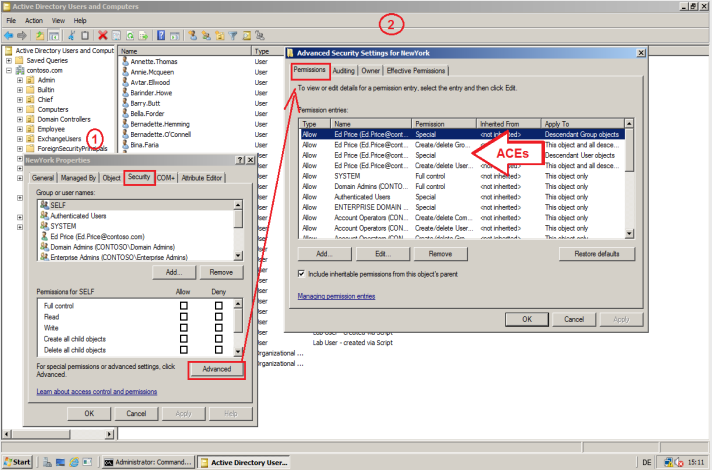
\includegraphics[width=6.26772in,height=2.18056in]{media/image108.png}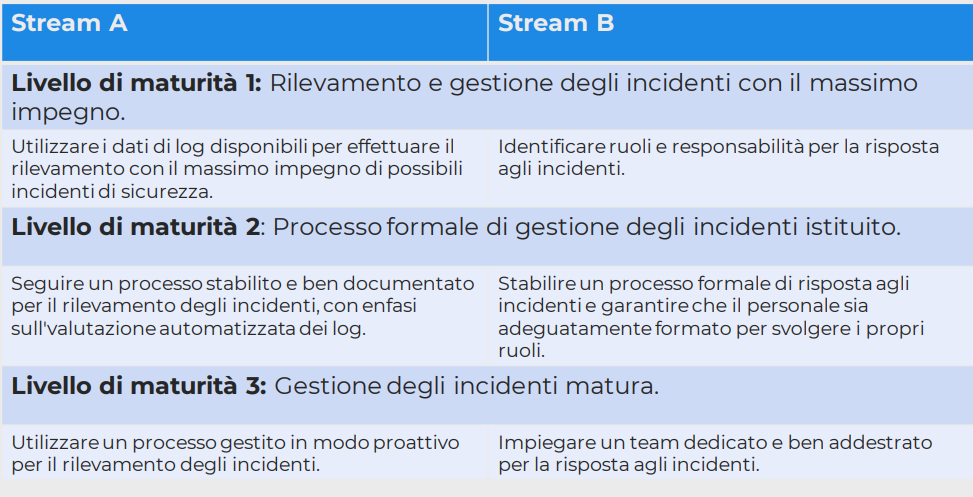
\includegraphics[width=6.26772in,height=3.41667in]{media/image74.png}

L'articolo 21 dice:

\emph{"Gli Stati membri provvedono affinché i soggetti essenziali e
importanti adottino misure tecniche, operative e organizzative adeguate
e proporzionate per gestire i rischi posti alla sicurezza dei sistemi
informatici e di rete che tali soggetti utilizzano nelle loro attività o
nella fornitura dei loro servizi, nonché per prevenire o ridurre al
minimo l\textquotesingle impatto degli incidenti per i destinatari dei
loro servizi e per altri servizi."}

Sostanzialmente tutti i soggetti indicati sopra devono prendere misure
per evitare rischi, queste misure sono definite e spiegate sempre
nell'articolo 21. Ecco alcuni esempi:

\begin{itemize}
\item
  Misura 3: continuità operativa, disaster recovery, ecc;
\item
  Misura 4: sicurezza della supply chain (catena di collaborazione fra
  aziende);
\item
  Misura 8: Crittografia e cifratura;
\item
  Misura 9: sicurezza risorse umane con controllo degli accessi e
  gestione utenti attivi (account di persone che non lavorano più li).
\end{itemize}

Un piano di adeguamento viene fatto per rendere conforme
un\textquotesingle azienda al NIS2, le fasi sono 4, nel dettaglio:

\begin{enumerate}
\def\labelenumi{\arabic{enumi}.}
\item
  \textbf{Analisi}: Per far si che la sicurezza si adatti all'azienda si
  fanno delle \emph{interviste e valutazioni}, è necessaria assoluta
  collaborazione fra tutti i soggetti per definire un piano di
  adeguamento efficace.
\item
  \textbf{Definizione}: \emph{Si definisce il piano completo tenendo in
  considerazione le criticità per il business individuate nelle fasi
  precedenti}, prioritizzando, così, le attività (es: definizione dei
  ruoli, definizione di KPI di sicurezza cioè un indice per diverse
  casistiche come il numero di attacchi ricevuti).
\end{enumerate}

\begin{quote}
Il NIS2 impone che anche aziende partner abbiamo lo stesso livello di
sicurezza.
\end{quote}

\begin{enumerate}
\def\labelenumi{\arabic{enumi}.}
\setcounter{enumi}{2}
\item
  \textbf{Implementazione:} si va ad \emph{implementare tutto quello
  concordato precedentemente}, per farlo dobbiamo capire quanto c'è di
  differenza tra dove siamo ora e dove vogliamo arrivare, questo spazio
  si dice gap e può essere:
\end{enumerate}

\begin{itemize}
\item
  \textbf{Gap Tecnologico}: comporta la necessità, comunemente, di
  aggiornare il sistema IT dal punto di vista sia infrastrutturale sia
  software.
\item
  \textbf{Gap Formativo}: è un grosso ostacolo per la corretta messa in
  atto del piano definito, pertanto è necessaria una formazione adeguata
  al ruolo che si ricopre.
\end{itemize}

\begin{enumerate}
\def\labelenumi{\arabic{enumi}.}
\setcounter{enumi}{3}
\item
  \textbf{Monitoraggio}: \emph{controllo che tutto sia rispettato},
  effettuare esami o simulazioni di attacco per vedere se i dipendenti
  sono preparati.
\end{enumerate}

Per vedere gli impatti andare nelle slides:

\textbf{Laboratorio di sicurezza dei sistemi informatici e privacy - 01
Normative - V1R0.pdf}

\href{https://liveunibo.sharepoint.com/:b:/s/LoPTSI_SedediImola/ET-eiun98a9BjHi7_UkTr2UBPhpsrulx9aFysJbld1LSZg?e=EHG2ot}{\textbf{\ul{Slides}}}

da pagina 82 a 90

\subsection{Regolamento DORA}\label{regolamento-dora}

Il Digital Operation Resilience Act (DORA), pacchetto europeo per la
digitalizzazione del settore finanziario, \emph{mira a garantire
adeguati meccanismi di salvaguardia in caso di attacchi informatici} e a
consolidare i requisiti per la \emph{prevenzione del rischio ICT nel
settore finanziario}

Pone particolare attenzione a cinque aree di sicurezza:

\begin{itemize}
\item
  Gestione del rischio ICT
\item
  Gestione del rischio ICT nei rapporti con terze parti
\item
  Governo della condivisione di informazioni tra entità finanziarie
\item
  Formulazione di reportistica legata a importanti incidenti ICT
\item
  Modalità di test per la verifica della resilienza digitale
\end{itemize}

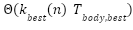
\includegraphics[width=6.26772in,height=3.30556in]{media/image59.png}

Il DORA è nato proprio per creare una regolamentazione a parte per
questo genere di enti per via della complessità di gestione e di
protezione.

Questa normativa non sostituisce altre normative preesistenti come NIS2
ma le integra, infatti il DORA è maggiormente orientato alla assicurarsi
la presenza di strategie, framework (modalità di lavoro che facilità) e
processi di governo.

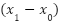
\includegraphics[width=6.26772in,height=3.625in]{media/image86.png}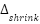
\includegraphics[width=6.26772in,height=0.58333in]{media/image98.png}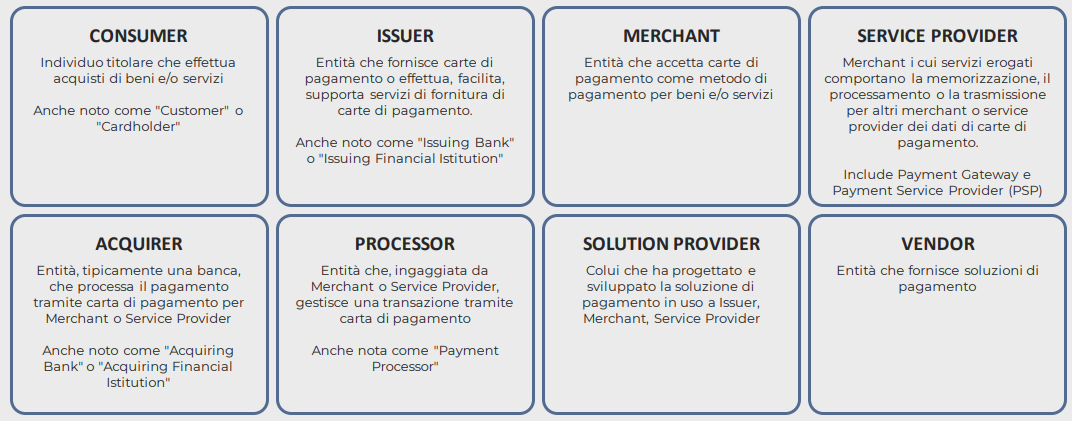
\includegraphics[width=6.26772in,height=0.77778in]{media/image38.png}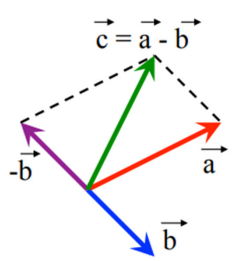
\includegraphics[width=6.26772in,height=0.61111in]{media/image67.png}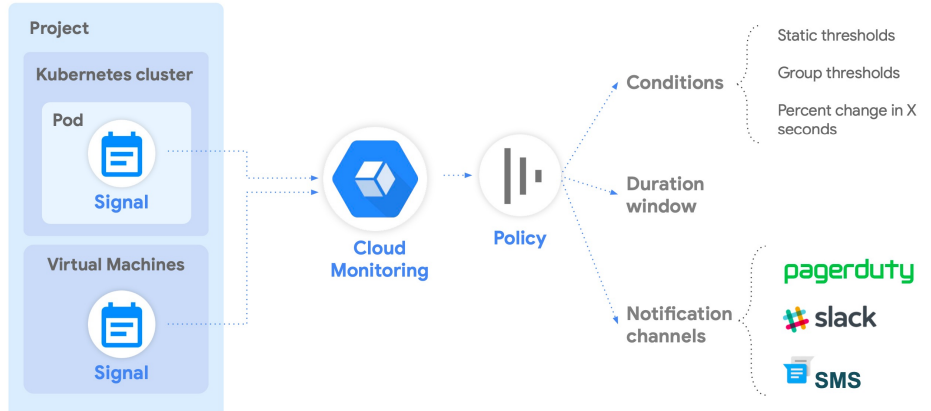
\includegraphics[width=6.26772in,height=0.43056in]{media/image28.png}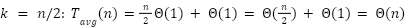
\includegraphics[width=6.26772in,height=0.65278in]{media/image77.png}

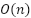
\includegraphics[width=6.26772in,height=3.25in]{media/image91.png}

\section{Active directory security}\label{active-directory-security}

Active Directory è un sistema server centralizzato, fondato sui concetti
di dominio e di directory, ovvero un insieme di servizi di rete, meglio
noti come directory service, gestiti da un domain controller. Tale
sistema, inoltre, definisce la modalità con cui vengono assegnate agli
utenti tutte le risorse di rete attraverso i concetti di: account
utente, account computer, cartelle condivise,.. secondo
l\textquotesingle assegnazione da parte
dell\textquotesingle amministratore di sistema di Group Policy.

Active Directory Service è un\textquotesingle infrastruttura informativa
condivisa per gestire elementi e risorse di rete in ambiente Windows,
tra le principali caratteristiche vi sono le seguenti:

\begin{itemize}
\item
  Erogazione di un archivio centrale per l\textquotesingle identità e le
  informazioni sull\textquotesingle account
\item
  Assegnazione di un identificatore univoco a ciascuno degli oggetti
\item
  Mappatura dei nomi delle risorse di rete ai loro rispettivi indirizzi
  di rete
\item
  Inclusione dei disposizioni di controllo dell\textquotesingle accesso,
  limitando la disponibilità delle informazioni della directory agli
  utenti autorizzati
\end{itemize}

\subsection{Architettura}\label{architettura}

Fisicamente, il sistema Active Directory è costituito da uno o più
Windows Server che eseguono un servizio chiamato Controller di dominio.

Un Directory Service è un servizio che archivia e organizza gli oggetti
in un archivio dati centralizzato e gerarchico:

\begin{itemize}
\item
  un oggetto directory è un oggetto che contiene uno o più attributi
\item
  gli oggetti sono identificati da un nome univoco, possono essere
  creati, aggiornati ed eliminati nella directory
\item
  I client possono recuperare il contenuto degli oggetti directory
  leggendo gli attributi di un oggetto specifico o eseguendo query per
  qualsiasi oggetto che corrisponda ai criteri specificati dal client
\end{itemize}

\subsection{Directory tree}\label{directory-tree}

Un concetto centrale nel servizio è la directory tree che possiede le
seguenti caratteristiche:

\begin{enumerate}
\def\labelenumi{\arabic{enumi}.}
\item
  Ogni oggetto ha un solo padre (tranne la radice
  dell\textquotesingle albero, il domain controller);
\item
  Ogni oggetto può avere zero o più oggetti figlio, dove a ciascuno
  viene assegnato un nome (RDN) univoco tra i fratelli;
\item
  Ogni oggetto della directory può essere identificato in modo univoco
  da tutti gli oggetti del servizio di directory dal suo nome distinto
  (DN), che si forma concatenandolo con l\textquotesingle RDN
  dell\textquotesingle oggetto.
\end{enumerate}

\subsection{Dominio}\label{dominio}

Un dominio è un insieme di utenti e computer che condividono una
namespace e un\textquotesingle infrastruttura di gestione comune. Tra le
caratteristiche della strutture vi è:

\begin{itemize}
\item
  la presenza di almeno un computer membro dell\textquotesingle insieme
  che funge da Domain Controller (DC) che ospita un elenco per
  identificare tutti i membri del dominio
\item
  la fruizione da parte del dominio di diversi servizi ai suoi client,
  principalmente relativi alla sicurezza e alla gestione
\item
  l' attuazione da parte del DC dell' autenticazione dei membri, creando
  un\textquotesingle unità di fiducia per i suoi membri
\item
  la condivisione del proprio identificativo tra tutti i membri
\end{itemize}

\subsection{Sicurezza}\label{sicurezza}

Esistono due oggetti fondamentali:

\begin{itemize}
\item
  Security Principal: è in identità associata ad un utente umano o ad un
  programma che può essere autenticato, tale identità deve possedere
  minimo due attributi: un nome e un id che lo identificano in modo
  univoco rendendolo significativo per il sistema.
\item
  Security Identifier (SID): È l'id per poter identificare il security
  principal ed è quello che viene controllato per accedere agli oggetti.
  Spesso il SID corrisponde ad un utente umano ma può anche essere un pc
  o un servizio
\end{itemize}

\subsubsection{Autenticazione/Autorizzazione}\label{autenticazioneautorizzazione}

Tutta l'infrastruttura permette agli utenti di effettuare l'accesso alle
informazioni richieste mediante un' autenticazione e un' autorizzazione:

\begin{itemize}
\item
  I security principals del dominio sono tutti disponibili nel domain
  controller
\item
  Il dominio funge da fonte primaria di identità per i clienti del
  dominio
\item
  Il dominio, attraverso i protocolli di sicurezza pertinenti, fornisce
  la base per l\textquotesingle autenticazione
  all\textquotesingle interno di esso
\item
  Durante il processo di autenticazione, il dominio fornisce
  informazioni di autorizzazione sotto forma di identità aggiuntive che
  rappresentano gruppi, consentendo di prendere decisioni di
  autorizzazione.
\end{itemize}

\subsubsection{LDAP}\label{ldap}

LDAP (Lightweight Directory Access Protocol) è un protocollo
multipiattaforma utilizzato per :

\begin{itemize}
\item
  autenticazione ai servizi di directory
\item
  comunicazione tra l\textquotesingle applicazione e i server dei
  servizi di directory che memorizzano e condividono informazioni su
  utenti, password e account di computer.
\end{itemize}

A causa dell\textquotesingle architettura di Active Directory, una volta
violato un computer collegato a un dominio, l\textquotesingle attaccante
può essere in grado di mappare la rete, individuare gli account e le
risorse sensibili e stimare le vulnerabilità. Tale processo è reso
possibile attraverso l'interrogazione del DC utilizzando il protocollo
LDAP.

Il protocollo consente diversi tipi di autenticazione (RFC 2829), per
esempio:

\begin{itemize}
\item
  Autenticazione anonima usata per disabilitare o aggiungere restrizioni
  di controllo degli accessi
\item
  Autenticazione nome/password (non sicura e non adatta se si vuole
  diritto di riservatezza)
\item
  Autenticazione mediante un digest (non espone la password in chiaro ma
  la password deve essere salvata in chiaro e precalcolato il digest
  lato server)
\item
  Autenticazione client basata su certificati
\end{itemize}

\subsection{Connessioni tra domini}\label{connessioni-tra-domini}

Ne esistono di diversi tipi:

\begin{itemize}
\item
  \textbf{Unidirezionali}: solo un dominio dei due della connessione, A
  e B, può accedere all'altro dominio; A accede a B ma non il contrario.
\item
  \textbf{Bidirezionale}: Il dominio A si fida del dominio B e il
  dominio B si fida del dominio A. Questa configurazione significa che
  le richieste di autenticazione possono essere tra i due domini in
  entrambe le direzioni. Alcune relazioni bidirezionali possono essere
  di due tipi (transitive o intransitive) a seconda del tipo di fiducia
  che si sta creando
\item
  \textbf{Transitivo}: può essere utilizzato per estendere le relazioni
  di fiducia con altri domini; se B si fida di C allora anche A può
  accedere a C perché si fida di B
\item
  \textbf{Intransitiva}: può essere utilizzata per negare le relazioni
  di fiducia con altri domini
\end{itemize}

\subsection{Strumenti di sicurezza}\label{strumenti-di-sicurezza}

\subsubsection{GPO}\label{gpo}

Un Group Policy Object (GPO) è un gruppo di impostazioni create
utilizzando la Microsoft Management Console (MMC). Le GPO possono essere
associate a uno o più contenitori di Active Directory, compresi siti,
domini o unità organizzative (UO). I Group Policy Object , se utilizzati
correttamente, consentono di aumentare la sicurezza dei computer degli
utenti, di difendersi dalle minacce interne e dagli attacchi esterni e,
in parte, di controllare ciò che gli utenti possono o non possono fare
su un sistema informatico.

\subsubsection{ACL}\label{acl}

Access Control Lists (ACLs) sono le impostazioni che definiscono le
autorizzazioni in Active Directory.

Ciascuna di esse deve definire:

\begin{itemize}
\item
  chi può accedere
\item
  a quale oggetto si può accedere
\item
  il tipo di accesso (ACE) Ogni ACE si riferisce al security principal
  (Utenti, Gruppi e Processi) e definisce i diritti di accesso
  all\textquotesingle oggetto (consentito o negato) per quel security
  principal. Inoltre le ACL sono molto flessibili e possono essere
  aggiunte altre ACE in base alle necessità.
\end{itemize}

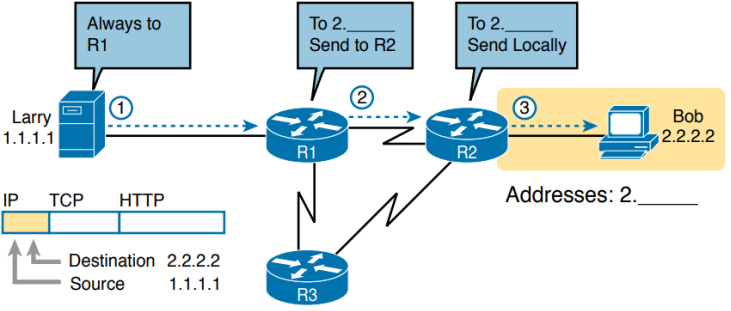
\includegraphics[width=6.26772in,height=4.13889in]{media/image106.png}

Un tipico ACE contiene le seguenti informazioni:

\begin{enumerate}
\def\labelenumi{\arabic{enumi}.}
\item
  Un identificatore di sicurezza (SID), unico in tutto il dominio
\item
  Una maschera di accesso(32 bit) che definisce le operazioni consentite
  o negate
\item
  Un flag che indica il tipo di ACE ( per consentire, per negare o di
  controllo di sistema)
\item
  Un insieme di flag che determinano se i contenitori o gli oggetti
  figli possono ereditare l'ACE del loro genitore
\end{enumerate}

\paragraph{Come funziona}\label{come-funziona}

Quando un mandante di sicurezza invia una Richiesta di accesso per un
oggetto, il SID della richiesta viene confrontato con
l\textquotesingle Elenco di controllo degli accessi.

Se il SID corrisponde al SID presente nell\textquotesingle ACL, al
mandante di sicurezza viene concesso l\textquotesingle accesso
all\textquotesingle oggetto in base ai diritti predefiniti (es. lettura,
scrittura, modifica, cancellazione, ecc.).

Esistono comunemente due tipi di ACL:

\begin{enumerate}
\def\labelenumi{\arabic{enumi}.}
\item
  Discretionary access control list (DACL) che definisce i principi di
  sicurezza che vengono concessi o negati.
\item
  System access control list (SACL) che garantisce agli admin il
  privilegio di registrare i log e i tentativi di accesso agli oggetti
  protetti
\end{enumerate}

\subsection{Aggiungere un PC}\label{aggiungere-un-pc}

Quando un pc è aggiunto a dominio cosa succede?

\begin{enumerate}
\def\labelenumi{\arabic{enumi}.}
\item
  Gli account utente del dominio diventano utenti validi del sistema e
  possono accedervi (a meno che non si applicano restrizioni).
\item
  Gli amministratori del dominio acquisiscono diritti amministrativi sul
  sistema.
\item
  Il computer stesso ottiene un account nel dominio e lo utilizza per
  autenticarsi.
\item
  Il nome del computer viene registrato nel DNS del dominio.
\item
  Le Group Policy definite nel dominio e indirizzate ai computer
  influiscono sul sistema.
\item
  Le Group Policy definite nel dominio e destinate agli utenti
  influiscono su qualsiasi utente del dominio che accede al computer.
\end{enumerate}

\subsection{NTLM}\label{ntlm}

Microsoft all' interno della propria architettura, dal 2008, ha creato
un protocollo di autenticazione, denominato NT LAN Manager (NTLM), che
consente l'autenticazione reciproca di computer e server diversi.

Il protocollo prevede l'autenticazione di un client mediante un nome
utente e una password associata attraverso uno scambio di informazioni
tra il dispositivo dell'utente e un server, il quale conosce i dati di
login e quindi può controllare l'accesso e autorizzarlo.

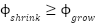
\includegraphics[width=6.26772in,height=2.88889in]{media/image107.png}

\subsubsection{Vantaggi}\label{vantaggi}

Un vantaggio di NTLM è che per l'autenticazione non bisogna inviare
sulla rete password non protette. La trasmissione dal client al server
avviene unicamente sotto forma di valore hash. Questo garantisce
certamente un maggiore livello di sicurezza.

\subsubsection{Svantaggi}\label{svantaggi}

Se il valore hash dovesse venir intercettato, può venir meno la
sicurezza promessa dal sistema. Infatti la password è crittografata
tramite MD4, un metodo crittografico considerato ormai poco sicuro in
quanto con i pc esistenti oggi tali valori hash possono essere
decodificati abbastanza facilmente attraverso un attacco brute force

\subsection{KERBEROS}\label{kerberos}

Kerberos, è un servizio di autenticazione che, consente autenticarsi
attraverso una rete insicura in maniera sicura, si assegna una chiave
unica a ciascun utente che si collega alla rete e incorporando poi
queste chiavi nei messaggi inviati dagli utenti (chiave simmetrica) e
per la verifica delle identità, si utilizzano delle codifiche
crittografate e una terza entità, responsabile della validazione
dell'autenticazione.

Il servizio è un progetto open source del Kerberos Consortium ed è la
tecnologia di autorizzazione standard di Microsoft Windows introdotta
già nelle prime apparecchiature di Windows 2000 in sostituzione di NTLM.
Kerberos gestisce l'autenticazione Single Sing On gestendo le
credenziali in tutta la foresta ogni volta che si cerca di accedere alle
risorse, dopo l'accesso iniziale al dominio tramite Winlogon.

\subsubsection{Funzionamento}\label{funzionamento}

\paragraph{Step 1}\label{step-1}

Client invia una richiesta (krb\_as\_req) all'AS chiedendo un Ticket per
accedere all'App Server. Tale richiesta è strutturata in questo modo:

\begin{itemize}
\item
  Timestamp (cifrato con user psw)
\item
  Username
\item
  Numero Causale scelto dall'utente (user\_nonce)
\item
  Nome del servizio richiesto(SPN)
\end{itemize}

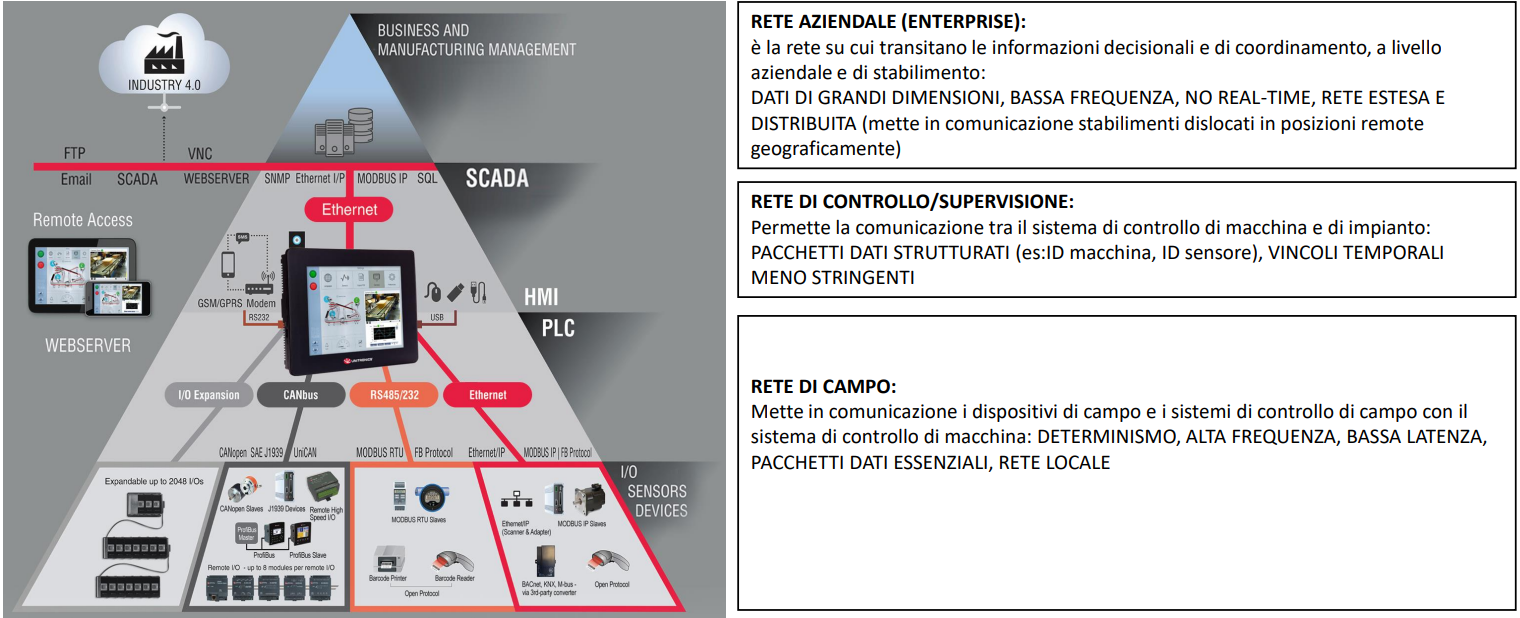
\includegraphics[width=3.23073in,height=2.13057in]{media/image40.png}

\paragraph{Step 2}\label{step-2}

Arrivata la richiesta all'AS recupera la password del client nel Db
utilizzando lo username e decifra l'intero msg verificando la sua
identità. Ed invia al client una risposta (KRB\_AS\_REP) che contiene:

\begin{enumerate}
\def\labelenumi{\arabic{enumi}.}
\item
  Username client in chiaro
\item
  II TGT (Ticket Granting Ticket) cifrato con una secret key
\item
  User data AS cifrato con la user psw
\end{enumerate}

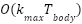
\includegraphics[width=3.75087in,height=2.4362in]{media/image62.png}

Il TGT è formato da:

\begin{itemize}
\item
  Username client
\item
  Session key - Data di scadenza del TGT
\item
  PAC (Priviledge Attribute Certificate) contenente le informazioni
  utili sui privilegi dell'utente
\end{itemize}

User Data AS invece contiene:

\begin{itemize}
\item
  Session key
\item
  Data di scadenza del TGT
\item
  User nonce
\end{itemize}

\paragraph{Step 3}\label{step-3}

Il client avendo ricevuto il TGT procede inviando la richiesta
(KRB\_TGS\_REQ ) di accesso al servizio al TGS.

Tale richiesta sarà formata da:

\begin{enumerate}
\def\labelenumi{\arabic{enumi}.}
\item
  Username e timestamp cifrato con la session key
\item
  Il TGT così com è perchè non conosce la chiave per decifrarlo
\item
  User nonce
\item
  Nome del servizio richiesto(SPN)
\end{enumerate}

\paragraph{Step 4}\label{step-4}

Il TGS ricevute le informazioni invia una risposta (KRB\_TGS\_REP ) al
Client contenente:

\begin{itemize}
\item
  Username in chiaro
\item
  Il Ticket Granting Service cifrato con un'altra secret key
\item
  User Data TGS cifrate con la session key
\end{itemize}

Il Ticket Granting Service è formato da:

\begin{itemize}
\item
  Username client - Service Session key
\item
  Data di scadenza del Ticket - PAC User Data TGS invece contiene:
\item
  Service Session key
\item
  Data di scadenza del Ticket
\item
  User nonce
\end{itemize}

Il Client ricevuto Il Ticket Granting Service e interpretando la service
session key invia all'App Server la richiesta di accesso alla risorsa
(KRB\_AP\_REQ) che contiene:

\begin{itemize}
\item
  Ticket granting service che non può decifrare non conoscendo la chiave
  di decifratura
\item
  Username e Timestamp cifrate con la service session key
\end{itemize}

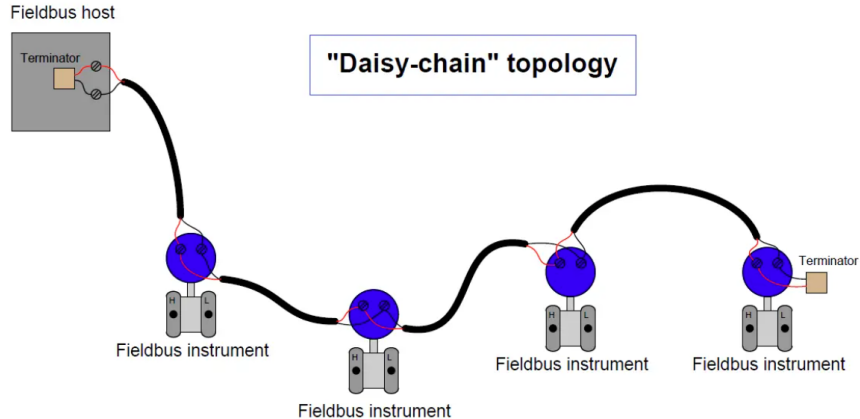
\includegraphics[width=4.19271in,height=2.59781in]{media/image118.png}

\paragraph{Step 5}\label{step-5}

L'App Server verifica il contenuto del Ticket Granting Service (più
precisamente interpreta il PAC) potendo decifrare entrambi in quanto è a
conoscenza di tutte le Secret Key essendo esse condivisa con il KDC.

E in caso di risposta affermativa dà il permesso al client di utilizzare
il servizio.

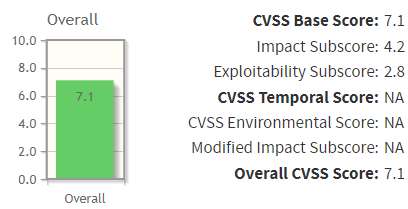
\includegraphics[width=4.03646in,height=2.40712in]{media/image27.png}

Per ricordare:

\emph{\textbf{Key Distribution Center (KDC)} è la terza entità che
verifica l'identità e rilascia i TGT.}

\emph{Comprende il TGS e AS.}

\emph{\textbf{Ticket Granting Ticket (TGT)} è il ticket che serve per
accedere al TGS e dimostrare che si è identificati.}

\emph{\textbf{Ticket Granting Service (TGS)} convalida il TGT e rilascia
un ticket per accedere ad un servizio.}

\subsubsection{Vantaggi}\label{vantaggi-1}

\begin{itemize}
\item
  Password non vengono mai inviate in rete in formato testuale.
\item
  Le ``chiavi segrete'' sono trasmesse nel sistema solo in forma
  criptata.
\item
  Tracciamento di chi ha richiesto che cosa e quando molto semplice
\item
  Il servizio permette inoltre agli utenti e ai sistemi di servizio di
  autenticarsi a vicenda.
\item
  A ogni passo del processo di autenticazione, sia gli utenti che i
  sistemi server sanno di avere a che fare con una controparte
  autentica.
\end{itemize}

\subsubsection{Svantaggi}\label{svantaggi-1}

\begin{itemize}
\item
  Kerberoasting
\item
  Golden Ticket e Silver Ticket
\item
  Le versioni più vecchie possono ancora essere utilizzate con la
  crittografia DES.
\item
  Replay attacks
\end{itemize}

\subsection{Kerberoasting}\label{kerberoasting}

Kerberoasting ci permette di decifrare le password degli account di
servizio per accedere a un dominio Active Directory come qualsiasi
utente autenticato.

Per farlo chiediamo al TGS ticket service (all'interno dell'Active
directory) per gli account di servizio specificando il loro valore SPN.
Quindi possiamo forzare questi ticket fino a quando non vengono violati,
senza alcun rischio di rilevamento o blocco
dell\textquotesingle account, ottenendo la password
dell\textquotesingle account.

\href{https://virtuale.unibo.it/pluginfile.php/2023963/mod_resource/content/1/Laboratorio\%20di\%20sicurezza\%20dei\%20sistemi\%20informatici\%20e\%20privacy\%20-\%2002\%20Active\%20Directory\%20Security\%20-\%20V1R0.pdf}{\ul{QUI
{[}37 - 41{]}}}

\subsection{Silver Ticket}\label{silver-ticket}

Attacco che comporta la compromissione delle credenziali e
l\textquotesingle abuso del design del protocollo Kerberos.

Consente a un utente malintenzionato di falsificare i TGS per servizi
specifici. I Tickets sono crittografati con l\textquotesingle hash della
password per il servizio; pertanto, se un attaccante ruba
l\textquotesingle hash per un account di servizio, può creare TGS Ticket
per quel servizio.

\href{https://virtuale.unibo.it/pluginfile.php/2023963/mod_resource/content/1/Laboratorio\%20di\%20sicurezza\%20dei\%20sistemi\%20informatici\%20e\%20privacy\%20-\%2002\%20Active\%20Directory\%20Security\%20-\%20V1R0.pdf}{\ul{QUI
{[}42 - 45{]}}}

\subsection{Golden Ticket}\label{golden-ticket}

Un Golden Ticket in Active Directory garantisce al beneficiario un
accesso illimitato alla risorsa tramite compromissione del protocollo
Kerberos.

Avviene quando un attaccante compromette l\textquotesingle hash della
password KRBTGT, nota solo al Key Distribution Center (KDC), e la
utilizza per emettere i biglietti Kerberos riuscendo ad accedere a
qualsiasi risorsa desiderata.

\href{https://virtuale.unibo.it/pluginfile.php/2023963/mod_resource/content/1/Laboratorio\%20di\%20sicurezza\%20dei\%20sistemi\%20informatici\%20e\%20privacy\%20-\%2002\%20Active\%20Directory\%20Security\%20-\%20V1R0.pdf}{\ul{QUI
{[}46 - 51{]}}}

La differenza principale tra un silver ticket e un golden ticket sta nel
livello di accesso che concedono a un utente non autorizzato.

\begin{itemize}
\item
  \textbf{Golden Ticket}: ticket di autenticazione Kerberos contraffatto
  che concede all\textquotesingle utente
  l\textquotesingle{}\emph{accesso a qualsiasi servizio nel dominio}.
  Viene creato falsificando un Ticket-Granting Ticket (TGT), che è il
  ticket iniziale che un utente ottiene dal Kerberos Authentication
  Server (KDC) dopo l\textquotesingle autenticazione. Un golden ticket è
  come una chiave passepartout che apre qualsiasi porta nel dominio.
\item
  \textbf{Silver Ticket}: ticket di autenticazione Kerberos contraffatto
  che concede all\textquotesingle utente l\textquotesingle accesso
  \emph{solo a un servizio specifico nel dominio}. Viene creato
  falsificando un Ticket-Granting Service (TGS) ticket, che è il ticket
  che un utente ottiene dal KDC per accedere a un servizio specifico. Un
  silver ticket è come una chiave contraffatta che apre solo una porta
  specifica nel dominio.
\end{itemize}

\section{Sicurezza applicativi web}\label{sicurezza-applicativi-web}

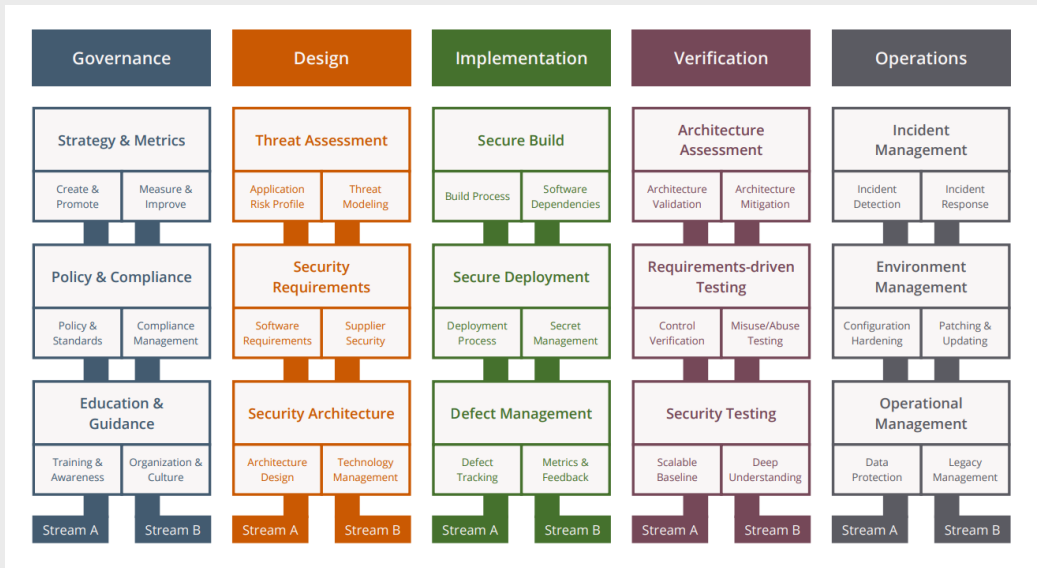
\includegraphics[width=6.26772in,height=2.33333in]{media/image109.png}

La sicurezza va valutata in ogni fase non solo nell'implementazione.

\subsection{Standard}\label{standard}

Ora vediamo una carrellata di standard di riferimento:

\begin{itemize}
\item
  \textbf{CERT Secure Coding Standard}: sviluppato appunto dal CERT e
  fra i vari principi si occupa di:

  \begin{itemize}
  \item
    prevenzione delle vulnerabilità;
  \item
    input validation (per evitare SQL injection) quindi controllo
    dell'input client/server side;
  \item
    sicurezza comunicazioni;
  \end{itemize}
\item
  \textbf{SSDF - Secure Software Development Framework}: del NIST è un
  quadro di riferimento completo per garantire la sicurezza del software
  durante tutto il ciclo di sviluppo mostrato sopra, con enfasi sulla
  fase di progettazione;
\item
  \textbf{PCI DSS - Payment Card Industry Data Security}: che dice come
  il software deve essere gestito per garantire un pagamento in rete
  sicuro;
\item
  \textbf{OWASP Application Security verification Standard}: è un
  framework + standard di sicurezza progettato per valutare delle
  applicazioni web e dei servizi web.
\end{itemize}

\subsection{Best practice}\label{best-practice}

\subsubsection{Deny by default}\label{deny-by-default}

Per accedere ad una determinata risorsa devi essere in whitelist, quindi
di base nessuno può accedere ed è il gestore che da il permesso a
ciascun individuo.

\subsubsection{Least privilege
principle}\label{least-privilege-principle}

Si riducono al minimo i privilegi di ogni utente per evitare che chi non
di dovere vada ad accedere a parti sensibili.

\subsubsection{Defense in Depth}\label{defense-in-depth}

Il principio è di mettere una sicurezza in più livelli in modo da
fermare un malintenzionato molto prima

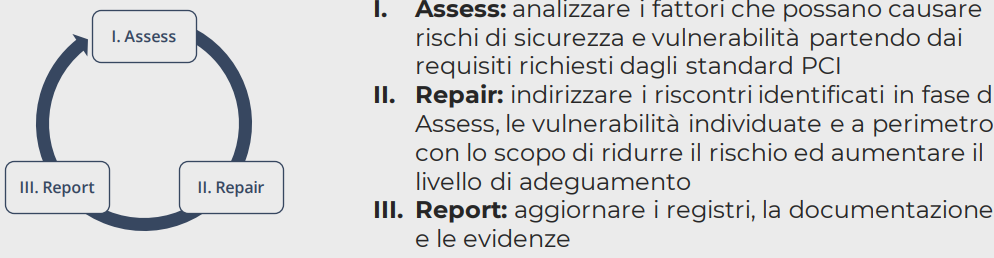
\includegraphics[width=6.26772in,height=2.86111in]{media/image39.png}

\subsubsection{Validate input}\label{validate-input}

Consiste nel verificare e garantire che i dati inseriti in
un\textquotesingle applicazione rispettino determinati criteri e regole.

La mancanza di una corretta validazione dell\textquotesingle input può
portare a vulnerabilità di sicurezza, quali attacchi di injection, e
compromettere l\textquotesingle integrità e la funzionalità
dell\textquotesingle applicazione.

Contiene la data sanitization.

\subsubsection{Compiler Warnings}\label{compiler-warnings}

I "compiler warnings" sono avvertimenti emessi durante la compilazione
del codice per segnalare possibili problemi o pratiche di programmazione
rischiose.

Fondamentali per garantire la sicurezza del software, spesso questi
messaggi identificano potenziali vulnerabilità, come
l\textquotesingle uso di variabili non inizializzate o conversioni di
tipo insicure, che potrebbero essere sfruttate in attacchi informatici.

\subsubsection{KISS}\label{kiss}

Acronimo che sta per ``Keep It Simple, Stupid'' che promuove la
scrittura di codice semplice e diretto senza complessità non necessaria.

\subsubsection{Data Sanitization}\label{data-sanitization}

Pulizia e validazione di dati per prevenire attacchi informatici.

Questo implica l\textquotesingle uso di tecniche come
l\textquotesingle escape dei caratteri speciali, la validazione dei
formati, il filtraggio dei caratteri pericolosi e
l\textquotesingle implementazione di query parametrizzate nei database.

\subsection{OWASP TOP10}\label{owasp-top10}

Comunità dedicata a indirizzare le organizzazioni nel sviluppare,
acquistare e mantenere applicazioni e API affidabili e sicure.

Tutti gli strumenti, i documenti, i video, le presentazioni e i capitoli
di OWASP sono gratuiti e aperti a chiunque sia interessato a migliorare
la sicurezza delle applicazioni.

La fondazione OWASP è l\textquotesingle ente no-profit che garantisce il
successo a lungo termine del progetto

Nel 2021 OWASP ha stilato una top 10 dei rischi di sicurezza più
problematici

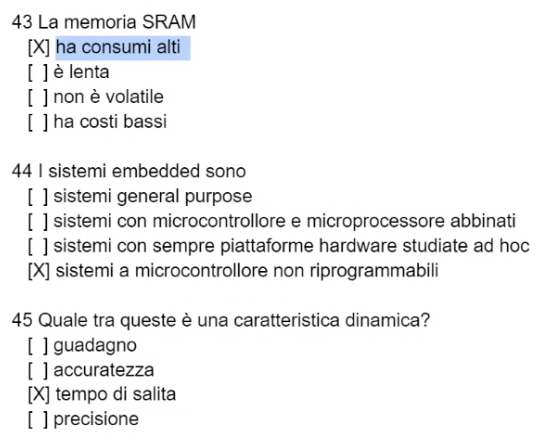
\includegraphics[width=6.26772in,height=4.27778in]{media/image8.png}

\subsubsection{Broken Access Control}\label{broken-access-control}

Il Broken Access Control si contestualizza all\textquotesingle interno
del processo di verifica dell\textquotesingle identità e della liceità
delle richieste, denominato controllo degli accessi e si concretizza
nella sua elusione o, comunque, nella modifica dei controlli
inizialmente implementati.

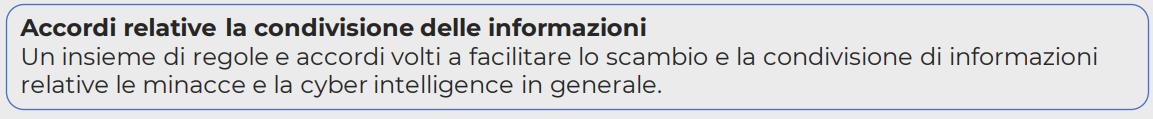
\includegraphics[width=6.26772in,height=2.61111in]{media/image88.png}

Le tipologie CWE sono le categorie di vulnerabilità CVE trovati.

L'incidenza indica quanti applicativi (nel pool analizzato) sono
vulnerabili a questa falla.

L'impatto medio delle vulnerabilità sull'applicativo.

L'exploitability medio è quanto è facile sfruttare le vulnerabilità.

Alcune nozioni per capire meglio la vulnerabilità:

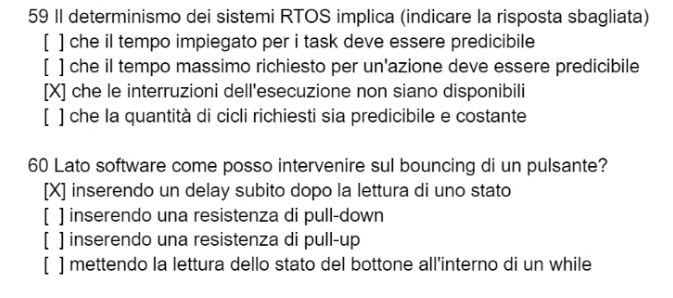
\includegraphics[width=6.26772in,height=2.51389in]{media/image21.png}

Il controllo degli accessi serve a garantire che gli utenti rispettino
le regole stabilite, impedendo loro di compiere azioni non
consentite.Quando ci sono problemi con questo tipo di controllo, possono
verificarsi situazioni indesiderate come la divulgazione non autorizzata
di informazioni, la manipolazione o la distruzione dei dati, oppure
l\textquotesingle esecuzione di funzioni aziendali al di là dei permessi
dell\textquotesingle utente. Bisogna stare attenti che le risorse che
difendiamo non siano accessibili da altri canali rendendo inutile il
controllo

La definizione formale è:

\emph{Il Broken Access Control è una categoria di vulnerabilità
ampiamente riscontrata in sistemi software, includendo anche applicativi
Web, che consiste in problemi legati ai permessi di accesso, aventi
impatto sulla sicurezza di sistemi, processi e informazioni.}

Nella tabella le principali contromisure riguardo broken access control:

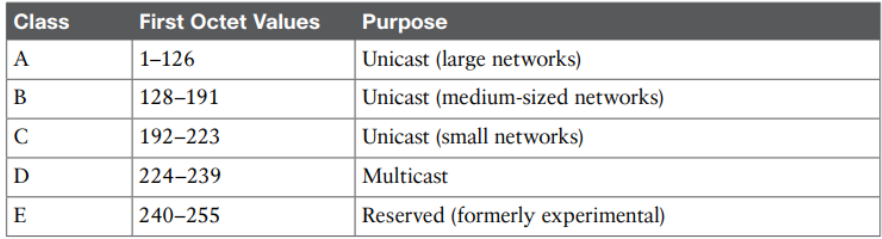
\includegraphics[width=6.26772in,height=2.83333in]{media/image84.png}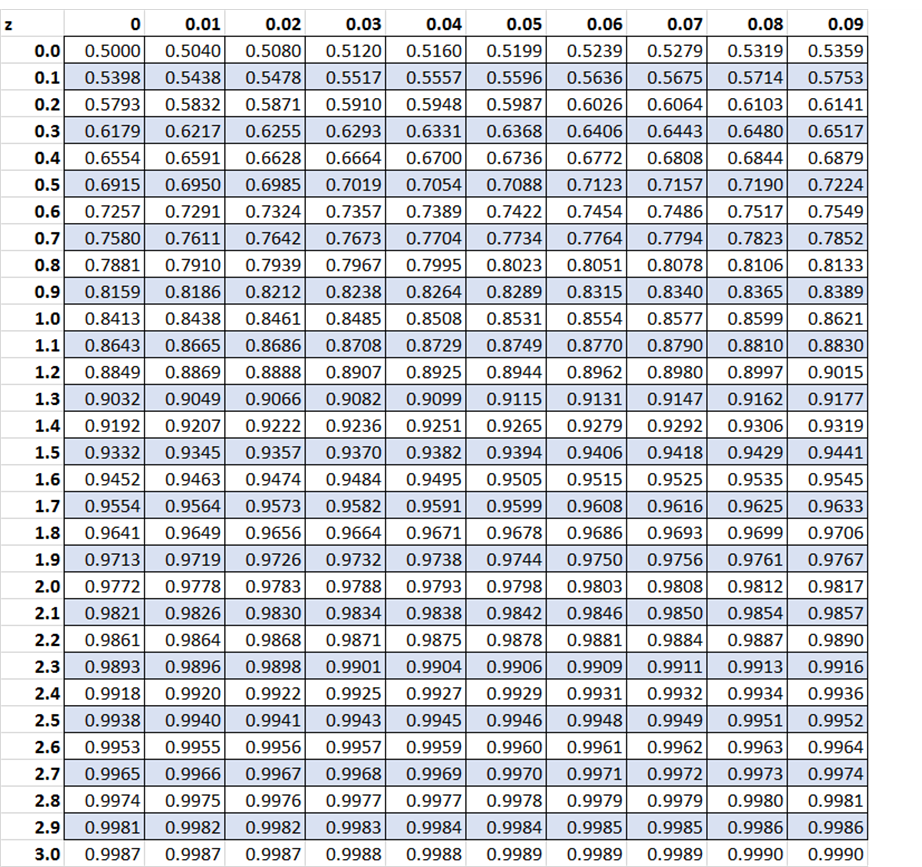
\includegraphics[width=6.26772in,height=2.47222in]{media/image9.png}

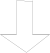
\includegraphics[width=5.75521in,height=3.10705in]{media/image41.png}

In conclusione:

\emph{Il Broken Access Control è, ad oggi, un rischio significativo.}

\emph{Per evitarlo, è cruciale seguire best practice di sicurezza
durante l\textquotesingle intero ciclo di vita del software, comprese le
fasi di analisi, progettazione e implementazione.}

\emph{È essenziale applicare principi come il privilegio minimo e
implementare un sistema solido di controllo degli accessi basato su
profili autorizzativi.}

\emph{L\textquotesingle identificazione e
l\textquotesingle autenticazione sicure sono misure fondamentali per
garantire l\textquotesingle efficacia dei processi autorizzativi.
Validazioni robuste, eseguite sia lato client sia lato server,
verificate ad ogni richiesta, risultano fondamentali.}

\subsubsection{Cryptographic failures}\label{cryptographic-failures}

I dati sensibili potrebbero essere esposti in diversi modi, tra questi
spiccano implementazioni crittografiche errate in modo parziale o
totale.

Errori legati alla crittografia spesso portano, infatti,
all\textquotesingle esposizione di dati sensibili o addirittura alla
compromissione del sistema, sia al momento della memorizzazione delle
informazioni, sia al momento dell'invio.

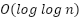
\includegraphics[width=5.77604in,height=2.40828in]{media/image90.png}

Alcune nozioni per capire meglio la vulnerabilità:

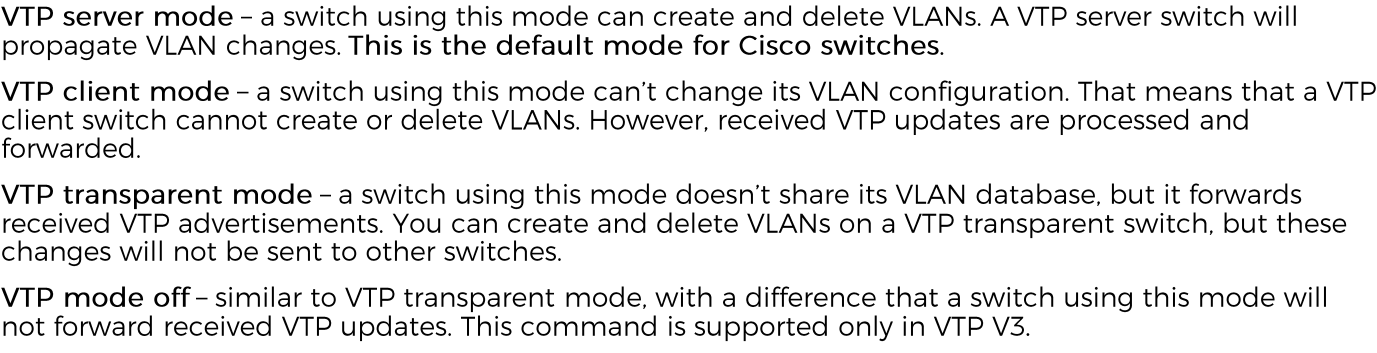
\includegraphics[width=6.26772in,height=2.52778in]{media/image22.png}

La definizione è:

\emph{Il Cryptographic Failures è una categoria di debolezze ampiamente
riscontrata in sistemi software, includendo anche applicativi web, che
consiste in problemi nella progettazione,
nell\textquotesingle implementazione o nell'uso di algoritmi e
protocolli crittografici, che causano impatti nella sicurezza di
sistemi, processi e informazioni.}

Il Cryptographic Failures di OWASP fornisce una guida dettagliata sugli
errori crittografici più comuni e pericolosi che possono verificarsi
nell\textquotesingle implementazione di funzionalità crittografiche
all\textquotesingle interno di un\textquotesingle applicazione, i
principali sono:

\begin{itemize}
\item
  Algoritmi crittografici deboli o insicuri: l\textquotesingle uso di
  algoritmi crittografici deboli o obsoleti può compromettere la
  sicurezza di un sistema. Ad esempio, l\textquotesingle impiego di
  algoritmi come DES o MD5 è considerato insicuro.
\item
  Problemi nella generazione e gestione delle chiavi: errori nella
  generazione, gestione o protezione delle chiavi crittografiche possono
  portare a vulnerabilità significative.
\item
  Utilizzo improprio della crittografia: implementazione erronea della
  crittografia, come l\textquotesingle uso di modalità insicure o la
  mancata applicazione di funzioni di hashing, può compromettere la
  protezione dei dati.
\item
  Mancanza di controllo dell'integrità dei dati: assenza di meccanismi
  per verificare l\textquotesingle integrità dei dati crittografati può
  consentire attacchi di manipolazione.
\item
  Problemi di implementazione del protocollo: errori
  nell\textquotesingle implementazione di protocolli crittografici, come
  TLS/SSL, possono portare all'esposizione totale di dati sensibili.
\end{itemize}

Nella tabella le principali contromisure riguardo cryptographic
failures:

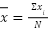
\includegraphics[width=6.26772in,height=3.08333in]{media/image54.png}

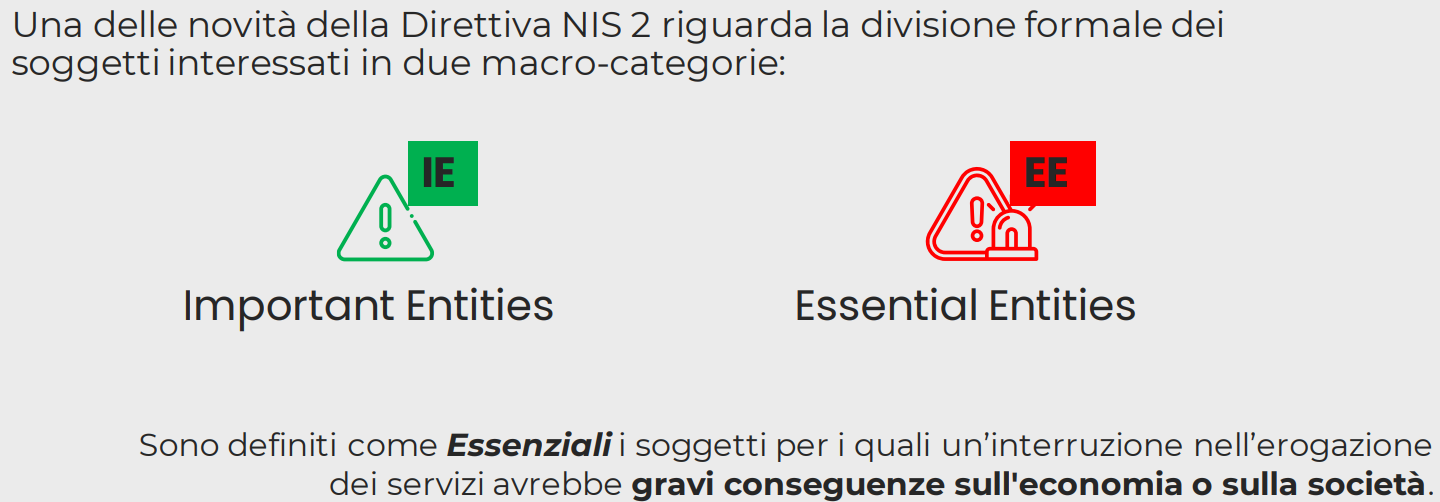
\includegraphics[width=5.94271in,height=3.42545in]{media/image104.png}

In conclusione:

\emph{Il Cryptographic Failures rappresenta una delle minacce più
rilevanti e pervasive nell\textquotesingle ambito della sicurezza delle
applicazioni Web. La crittografia svolge un ruolo cruciale nella
protezione dei dati sensibili e nella garanzia
dell\textquotesingle integrità delle comunicazioni, ma errori nella sua
implementazione possono comportare gravi conseguenze.}

\emph{Il Cryptographic Failures può mettere a rischio la confidenzialità
dei dati e la sicurezza delle applicazioni.}

\subsubsection{Injection}\label{injection}

Le vulnerabilità di tipo injection vedono la loro causa primaria nella
gestione incorretta dei dati di input.

Gli attacchi di tipo injection si differenziano in base alla tecnologia
colpita e alle modalità di esecuzione dell'attacco (SQL injection, OS
command injection, Cross Site Scripting (XSS)).

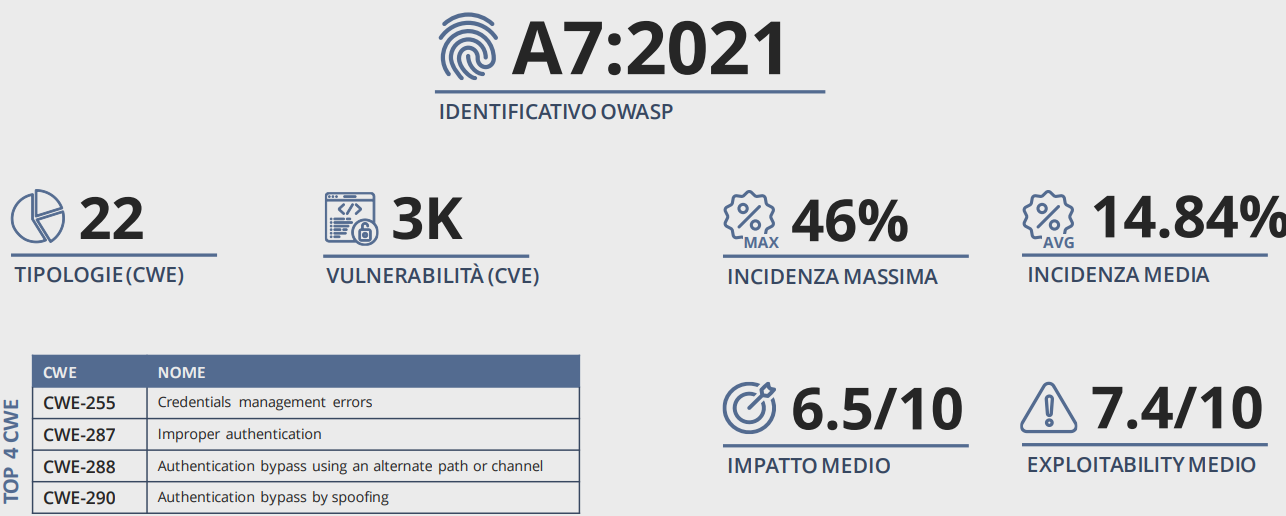
\includegraphics[width=6.26772in,height=2.83333in]{media/image94.png}

Alcune nozioni per capire meglio la vulnerabilità:

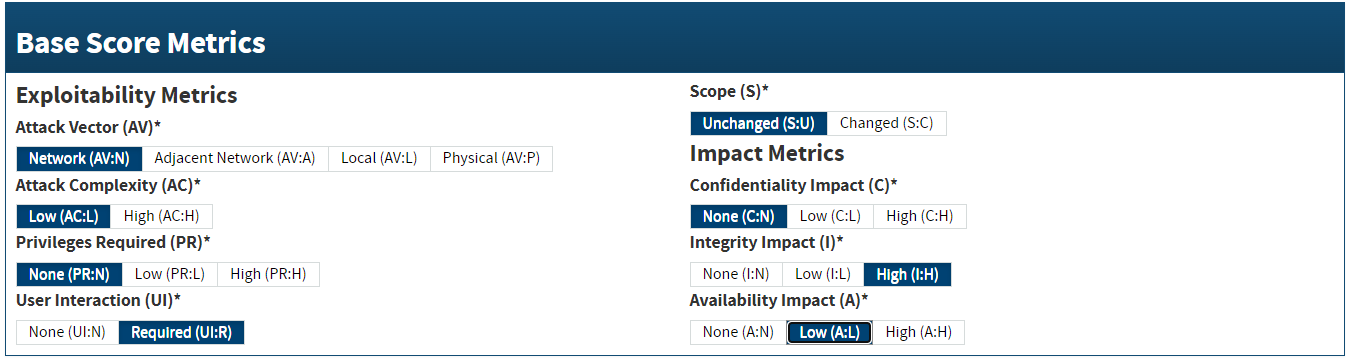
\includegraphics[width=5.37911in,height=2.16865in]{media/image26.png}

La definizione è:

\emph{L\textquotesingle Injection è una tecnica di attacco informatico
che consiste nell'inserimento di codice malevolo in un'applicazione, in
un processo in esecuzione o in un database, al fine di modificarne il
comportamento previsto.}

Gli attacchi di tipo injection, variegati e strettamente legati alla
tecnologia coinvolta, condividono il concetto fondamentale: manipolare
la logica di esecuzione dell\textquotesingle applicativo attraverso
l\textquotesingle inserimento di input controllato
dall\textquotesingle utente malintenzionato.

Ad esempio, i buffer overflow sfruttano l\textquotesingle inserimento di
una quantità eccessiva di dati per sovrascrivere parti del codice,
potenzialmente compromettendo il servizio e permettendo
l\textquotesingle esecuzione di codice malevolo. La radice del problema
risiede nella mancanza di controlli sull\textquotesingle input; è
essenziale verificarne la conformità alle aspettative e considerare non
valido l\textquotesingle input non conforme.

Nella tabella le principali contromisure riguardo injection:

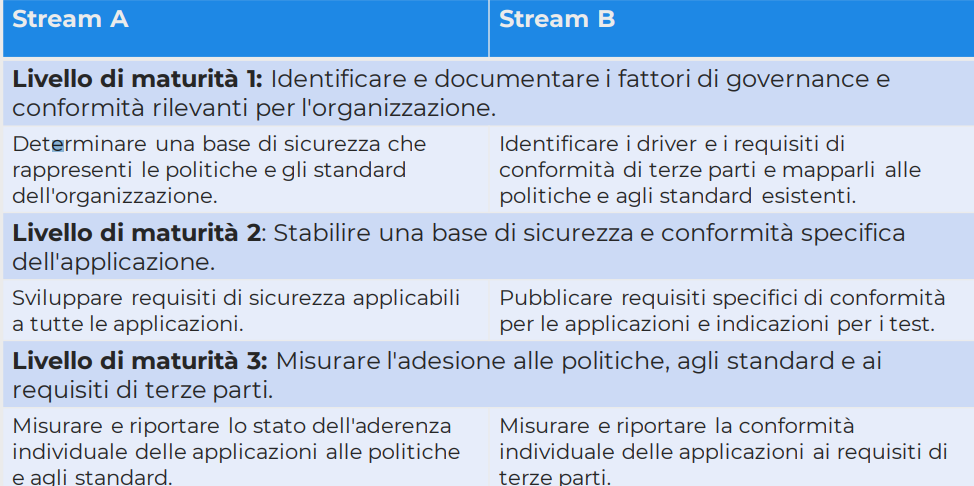
\includegraphics[width=6.26772in,height=2.125in]{media/image87.png}

\includegraphics[width=6.26772in,height=3.15278in]{media/image92.png}

\subsubsection{Insecure design}\label{insecure-design}

Si concentra sui rischi associati ai difetti di progettazione e
architetturali. In particolare, questa categoria si dedica al threat
modeling, all\textquotesingle utilizzo di design-pattern sicuri e alle
scelte architetturali.

Uno dei fattori che contribuisce all'insecure design è la mancanza di un
profilo di rischio a livello di business, che comporta una carenza di
conoscenza dei livelli di sicurezza necessari.

Un design insicuro rimane vulnerabile anche in assenza di bug, poiché
per sua natura manca delle protezioni necessarie a livello progettuale.
Le conseguenze di una possibile falla nel design dipendono fortemente
dall\textquotesingle origine del problema, ovvero dalla mancanza a
livello progettuale. Tali conseguenze possono tradursi in ingenti
perdite economiche, poiché risolvere una lacuna a livello progettuale
richiede uno sforzo significativo.

\includegraphics[width=6.26772in,height=2.63889in]{media/image76.png}

Alcune nozioni per capire meglio la vulnerabilità:

\includegraphics[width=6.26772in,height=2.66667in]{media/image78.png}

La definizione è:

\emph{L\textquotesingle Insecure Design si riferisce a un approccio di
progettazione che presenta vulnerabilità e lacune nella sicurezza di un
sistema, applicazione o prodotto. Questo tipo di design manca di
controlli e misure di sicurezza efficaci, aumentando il rischio di
esposizione a minacce informatiche e violazioni della sicurezza.}

Nella tabella le principali contromisure riguardo insecure design:

\includegraphics[width=6.26772in,height=2.91667in]{media/image60.png}

\includegraphics[width=6.26772in,height=3.20833in]{media/image112.png}

\subsubsection{Security
misconfiguration}\label{security-misconfiguration}

la Security Misconfiguration, circa il 90\% di applicazioni testate sono
risultate vulnerabili ad essa. Non sorprende vedere questa categoria
così rilevante, essendo i software sempre più configurabili e, spesso,
lasciati dall'utente allo stato di default.

\includegraphics[width=6.26772in,height=2.52778in]{media/image11.png}

\includegraphics[width=6.28646in,height=2.75228in]{media/image97.png}

La definizione è:

\emph{La Security Misconfiguration è una categoria di vulnerabilità che
si verifica quando un\textquotesingle applicazione, un server o
qualsiasi componente di un sistema è configurato in modo errato,
lasciando aperte vulnerabilità che potrebbero essere sfruttate dagli
aggressori.}

Tali configurazioni di sicurezza errate possono manifestarsi in vari
modi, ad esempio:

\begin{itemize}
\item
  Permissive Configurations: Assegnare permessi eccessivi o non
  necessari a utenti, processi o risorse, consentendo
  l\textquotesingle accesso non autorizzato o il potenziale sfruttamento
  di vulnerabilità.
\item
  Insecure Defaults: Utilizzare impostazioni di default che sono
  intrinsecamente insicure. Ciò potrebbe includere password deboli,
  configurazioni di crittografia insoddisfacenti o altre scelte di
  configurazione che rendono il sistema vulnerabile.
\item
  Exposed Sensitive Information: Rivelare informazioni sensibili o
  dettagli implementativi nel codice, nei file di configurazione o
  altrove. Queste informazioni potrebbero essere sfruttate dagli
  aggressori per pianificare e condurre attacchi più mirati.
\end{itemize}

Nella tabella le principali contromisure riguardo la security
misconfiguration:

\includegraphics[width=6.26772in,height=3.02778in]{media/image116.png}

\includegraphics[width=6.26772in,height=4.41667in]{media/image105.png}

La Security Misconfiguration è una delle principali minacce alla
sicurezza delle applicazioni Web e dei sistemi in generale. Gli
attaccanti possono sfruttare configurazioni errate per ottenere accesso
non autorizzato, eseguire attacchi di traversing directory, scoprire
informazioni sensibili e altro ancora.

È essenziale eseguire regolarmente audit di sicurezza e revisioni delle
configurazioni per identificare e correggere eventuali vulnerabilità di
configurazione.

\subsubsection{Vulnerable and outdated
components}\label{vulnerable-and-outdated-components}

La categoria Vulnerable and Outdated Components di OWASP riguarda una
problematica nota, per la quale risulta complesso effettuare dei test
mirati e, pertanto calcolarne il rischio.

È infatti l'unica categoria per cui non è associato nessun Common
Vulnerability and Exposure (CVE).

\includegraphics[width=6.26772in,height=2.33333in]{media/image114.png}

\includegraphics[width=6.26772in,height=2.75in]{media/image119.png}

La definizione è:

\emph{Il Vulnerable and Outdated Components è una minaccia alla
sicurezza che si verifica quando un\textquotesingle applicazione
utilizza componenti software, come librerie o framework, che contengono
vulnerabilità di sicurezza note o sono datati e non più supportati.}

Si vuole sottolineare, inoltre, che le applicazioni spesso dipendono da
componenti di terze parti per funzionare in modo efficiente. Tali
componenti potrebbero contenere vulnerabilità di sicurezza o potrebbero
essere obsolete. In tal caso, possono costituire una potenziale via di
accesso per gli attaccanti. Gli aggressori possono sfruttare le
vulnerabilità nelle versioni obsolete o noti problemi di sicurezza nelle
componenti utilizzate per compromettere l\textquotesingle applicazione
e, in ultima analisi, il sistema sottostante.

Il Vulnerable and Outdated Components di OWASP si presenta se:

\begin{itemize}
\item
  Non si conoscono le versioni di tutti i componenti utilizzati (sia
  lato client che lato server). Questo include i componenti utilizzati
  direttamente così come le dipendenze annidate.
\item
  Se il software è vulnerabile, non supportato o non aggiornato. Questo
  include i sistemi operativi, i server web, i database management
  system (DBMS), le applicazioni, API e tutti i componenti, ambienti di
  esecuzione e librerie.
\item
  In caso non venissero effettuate scansioni periodiche di sicurezza e
  non si consultassero i bollettini di sicurezza relativi ai componenti
  utilizzati.
\item
  In caso non fosse previsto un piano efficace di patch management
  relativamente alla piattaforma sottostante, i framework, e le
  dipendenze in modo tempestivo e basato sul rischio.
\item
  In assenza di test di specifici per verificare la non regressione del
  software a seguito di aggiornamenti di librerie.
\end{itemize}

Nella tabella alcune contromisure:

\includegraphics[width=6.26772in,height=3.04167in]{media/image65.png}

\subsubsection{Identification and authentication
failures}\label{identification-and-authentication-failures}

Precedentemente denominata Broken Authentication. Questo termine si
riferisce a una serie di vulnerabilità e inefficienze che possono
emergere nei processi di identificazione e autenticazione, i quali sono
fondamentali per garantire l\textquotesingle accesso sicuro e
autorizzato ai sistemi e alle applicazioni.

\includegraphics[width=6.26772in,height=2.51389in]{media/image93.png}

\includegraphics[width=6.26772in,height=2.88889in]{media/image15.png}

La definizione è:

\emph{Identification and Authentication Failures riguarda situazioni in
cui i meccanismi di autenticazione e identificazione di
un\textquotesingle applicazione non sono implementati in modo sicuro o
sono vulnerabili. Questo può includere problemi come la gestione
inadeguata delle sessioni, l\textquotesingle uso debole di password, la
mancanza di controlli di autenticazione multi-fattore, errori nelle
risposte di autenticazione e altri problemi legati
all\textquotesingle identificazione e alla verifica delle identità degli
utenti.}

Nella tabella alcune contromisure:

\includegraphics[width=4.63698in,height=1.98868in]{media/image115.png}

\includegraphics[width=6.26772in,height=3.20833in]{media/image17.png}

\subsubsection{Software and data integrity
failures}\label{software-and-data-integrity-failures}

Si focalizza sulle relazioni di fiducia senza verifiche di integrità in
contesti di aggiornamento software, gestione di dati critici e CI/CD
pipelines.

\includegraphics[width=6.26772in,height=2.69444in]{media/image14.png}

\includegraphics[width=6.26772in,height=2.72222in]{media/image24.png}

La definizione è:

\emph{La classe di vulnerabilità Software and Data Integrity Failures
secondo i dati forniti è caratterizzata da situazioni in cui il codice e
l\textquotesingle infrastruttura non proteggono adeguatamente contro
violazioni dell\textquotesingle integrità del software e dei dati.}

\emph{Queste vulnerabilità possono derivare da pratiche come
l\textquotesingle inclusione di funzionalità da fonti non attendibili,
la mancanza di verifica dell\textquotesingle integrità durante gli
aggiornamenti del software, e la presenza di vulnerabilità di
deserializzazione non sicura.}

Nella tabella alcune contromisure:

\includegraphics[width=6.26772in,height=3in]{media/image64.png}

\includegraphics[width=6.26772in,height=3.93056in]{media/image53.png}

\includegraphics[width=6.26772in,height=2.86111in]{media/image101.png}

La gestione delle vulnerabilità di software e integrità dei dati
richiede un approccio strategico. L\textquotesingle implementazione di
firme digitali, controlli di accesso e la verifica delle dipendenze sono
essenziali per mitigare rischi come l\textquotesingle esecuzione di
codice malevolo o la compromissione dei dati.

Processi di revisione e monitoraggio continuo sono fondamentali per
individuare e correggere potenziali vulnerabilità.
L\textquotesingle adozione di pratiche sicure nella catena di
distribuzione del software, inclusa la protezione delle pipeline CI/CD,
contribuisce a prevenire accessi non autorizzati e modifiche
indesiderate.

Mantenere le librerie e i framework aggiornati è cruciale per
beneficiare delle ultime correzioni di sicurezza. In sintesi, un
approccio completo e proattivo è essenziale per garantire la robustezza
e l\textquotesingle integrità dei sistemi software.

\subsubsection{Security logging and monitoring
failures}\label{security-logging-and-monitoring-failures}

Una delle principali sfide nella sicurezza delle applicazioni riguarda
l'insufficienza o la totale mancanza di logging e monitoraggio.

\includegraphics[width=6.26772in,height=2.51389in]{media/image47.png}

\includegraphics[width=6.26772in,height=2.91667in]{media/image48.png}

La definizione è:

\emph{I Security Logging and Monitoring Failures si presentano quando
non viene svolto in maniera efficace un monitoraggio di attività
sospette o potenzialmente dannose. Le applicazioni sicure, infatti,
devono essere in grado di registrare in modo adeguato le attività
rilevanti, come gli eventi di sicurezza, gli accessi, le modifiche e
altri comportamenti significativi.}

Nella tabella alcune contromisure:

\includegraphics[width=6.26772in,height=3.20833in]{media/image36.png}

\includegraphics[width=6.26772in,height=3.40278in]{media/image55.png}

\subsubsection{Server-side request
forgery}\label{server-side-request-forgery}

\includegraphics[width=6.26772in,height=2.375in]{media/image73.png}

\includegraphics[width=6.26772in,height=2.375in]{media/image79.png}

La definizione è:

\emph{Il Server-Side Request Forgery (SSRF) è un vettore di attacco che
sfrutta un\textquotesingle applicazione per interagire con la rete
interna/esterna o la macchina stessa. Si manifesta attraverso
l\textquotesingle errata gestione degli URL. Questo può coinvolgere
immagini su server esterni, Web Hook personalizzati e richieste interne
per interagire con altri servizi.}

Il flusso comune di SSRF coinvolge la prima richiesta, spesso HTTP,
seguita da una seconda richiesta che può utilizzare diversi protocolli e
schemi.

A seconda delle funzionalità e dei requisiti
dell\textquotesingle applicazione, SSRF può verificarsi in due casi
principali:

\begin{itemize}
\item
  Vincolo di Dominio/IP Identificato e Fidato:
\item
  l\textquotesingle applicazione può inviare richieste solo a domini o
  IP identificati e fidati. o Libero Accesso a IP o domini esterni:
  l\textquotesingle applicazione può inviare richieste a qualsiasi
  indirizzo IP o nome di dominio esterno.
\end{itemize}

Nella tabella alcune contromisure:

\includegraphics[width=6.26772in,height=3.11111in]{media/image34.png}\includegraphics[width=6.26772in,height=3.31944in]{media/image32.png}\includegraphics[width=6.26772in,height=3.5in]{media/image19.png}

La gestione efficace delle vulnerabilità SSRF richiede una strategia
bilanciata, adottando una doppia strategia.

A livello di rete, implementare regole firewall "deny by default" e
suddividere le reti per limitare l\textquotesingle accesso.

Sul fronte applicativo, usare le allow list per ridurre il rischio. In
scenari di comunicazione con risorse specifiche, le allow list sono
efficaci. Un'alternativa alle allow list sono i token di sicurezza,
poiché garantiscono un altro livello di sicurezza.

La consapevolezza del personale è cruciale, evita input URL completi e
garantisce la conformità ai protocolli. Un approccio integrato tra rete
e applicazione è essenziale per difendersi da minacce SSRF.

\section{Crittografia}\label{crittografia}

Disciplina che racchiude i principi/mezzo per trasformare i dati al fine
di nasconderne il contenuto e impedirne l'uso e modifiche non
autorizzate.

Garantisce:

\begin{itemize}
\item
  confidenzialità: i dati non vengono visti da chi non autorizzato;
\item
  integrità: i dati non vengono alterati;
\item
  autenticità: si è certi che i dati provengono davvero dalla fonte.
\end{itemize}

Alcune terminologie:

\begin{itemize}
\item
  Messaggio in chiaro: il messaggio di partenza che si vuole proteggere
  con cifratura
\item
  Messaggio cifrato: output di un algoritmo di crittografia, appare con
  una serie di cifre casuali.
\item
  Chiave: Un parametro utilizzato da un algoritmo per effettuare
  un'operazione crittografica (es. cifratura di un messaggio in chiaro o
  decifratura di un messaggio cifrato). È detta pubblica se è possibile
  divulgarla pubblicamente senza compromettere la sicurezza dei dati
  cifrati, privata altrimenti.
\item
  Schema crittografico: insieme di trasformazioni specificate senza
  ambiguità che richiede la collaborazione di due o più parti al fine di
  ottenere un servizio (crittografico).
\item
  Security strength: numero, indicato in bit, che indica la quantità di
  lavoro necessaria per violare un algoritmo crittografico; se il suo
  valore è S bit sono necessari \(2^{S}\) operazioni.
\item
  Criptoperiodo: L\textquotesingle arco di tempo in cui una determinata
  chiave è autorizzata all\textquotesingle uso o in cui le chiavi di un
  determinato sistema possono rimanere in vigore.
\end{itemize}

\subsection{Algoritmi a chiave
simmetrica}\label{algoritmi-a-chiave-simmetrica}

Classe di algoritmi dove viene definita e usata una sola chiave per
cifrare e decifrare, è necessario condividerla fra attori della
comunicazione.

Vantaggi:

\begin{itemize}
\item
  Alta efficienza in termini di costo computazionale
\item
  Accelerazione hardware presente all'interno della maggior parte delle
  CPU moderne
\item
  Le quantità di dati cifrabili con una chiave sono molto ampie
\end{itemize}

Svantaggi:

\begin{itemize}
\item
  Soffrono del problema dello scambio della chiave: per iniziare una
  comunicazione sicura, è necessario avere a disposizione una chiave
  condivisa con la controparte
\end{itemize}

\subsubsection{Cifratura a blocchi}\label{cifratura-a-blocchi}

L'algoritmo divide i dati da cifrare in blocchi di dimensione fissa,
successivamente con la chiave cifriamo e decifriamo ciascun blocco.

\subsubsection{Cifratura a flusso}\label{cifratura-a-flusso}

Tramite la chiave simmetrica generiamo un flusso di bit pseudo-casuali,
ogni bit del messaggio in chiaro verrà messo a XOR con il flusso appena
ottenuto. Per decifrare facciamo le stesse operazioni.

Un problema è che un malintenzionato potrebbe modificare il messaggio
originale andando a cambiare un simbolo del testo cifrato.

\subsubsection{Operazioni cifrari a
blocchi}\label{operazioni-cifrari-a-blocchi}

Prima di vedere le operazioni vediamo due definizioni:

\begin{itemize}
\item
  Nonce: valore che deve essere utilizzato una volta sola. Deve essere
  diverso per ogni comunicazione, tuttavia non ha altri tipi di
  requisiti.
\item
  Initialization Vector: deve essere casuale e non deve avere nessun
  tipo di legame con gli IV utilizzati in comunicazioni passate.
\item
\end{itemize}

Per esempio, se un cifrario richiede l'utilizzo di un Nonce, potremo
generare un valore casuale per la prima comunicazione e incrementarlo di
un valore fisso per tutte le comunicazioni successive. Questo non
sarebbe possibile con un cifrario che richiede l'utilizzo di un IV,
perciò sarebbe necessario generare una valore casuale ad ogni nuova
comunicazione, altrimenti il livello di sicurezza offerto dall'algoritmo
sarebbe compromesso.

\paragraph{ECB}\label{ecb}

Electronic Code Block, ogni blocco viene cifrato con la stessa chiave,
avendo poi più blocchi cifrati uguali, per questo non si consiglia di
utilizzare la stessa chiave per ogni blocco rendendo il cifrario debola
ad attacchi basati su crittoanalisi.

\paragraph{CBC}\label{cbc}

Cipher Block Chaining, il primo blocco in chiaro viene messo a XOR con
un initialization vector, ottenendo un blocco cifrato che verrà messo a
XOR con il prossimo in chiaro e così via.

\paragraph{CFB}\label{cfb}

Cipher Feedback Mode, si genera un cifrario a blocchi (creato da chiave
e initialization vector) che si mette a XOR con il primo blocco in
chiaro ottenendo un blocco cifrato, successivamente si rigenera il
cifrario a blocchi con il blocco appena creato e la chiave, che verrà
messo a XOR con il prossimo blocco non cifrato, e così via.

\includegraphics[width=6.26772in,height=0.875in]{media/image23.png}

\paragraph{OFB}\label{ofb}

Output Feedback Mode, come il precedente ma invece di utilizzare il
blocco cifrato per creare un altro cifrario a blocchi ma utilizziamo il
cifrario appena utilizzato con la chiave per crearne uno nuovo.

In questo modo non propaghiamo errori in un bit su tutto il messaggio.

\includegraphics[width=6.26772in,height=0.875in]{media/image80.png}

\paragraph{CTR}\label{ctr}

Counter mode, utilizziamo un nonce, uguale per tutti i blocchi, e un
contatore unico per ciascun blocco.

Il nonce e il contatore vengono cifrati con il cifrario a blocchi;
l'output viene messo a XOR con il blocco in chiaro per generare il
blocco cifrato.

Il vantaggio che questa modalità offre è la possibilità di
parallelizzare completamente la cifratura dei vari blocchi in quanto non
c'è nessuna dipendenza fra i diversi blocchi.

\subsubsection{Data at rest e data in
transit}\label{data-at-rest-e-data-in-transit}

Data at rest intende le info. memorizzate su un dispositivo o database,
i data in transit intende i dati mentre sono trasmessi.

\subsubsection{XTS}\label{xts}

Modalità per proteggere specificamente i dati at rest.

Utilizza due chiavi:

\begin{itemize}
\item
  principale: uguale per tutti i dati;
\item
  specifica: per ogni blocco (si utilizza il numero di settore).
\end{itemize}

\subsubsection{Authenticated Encryption}\label{authenticated-encryption}

Fornisce una classe di algoritmi detta Authenticated Encryption with
Associated Data (AEAD). La parte del nome Associated Data fa riferimento
alla possibilità di includere nel messaggio una parte di dati che non
verranno cifrati.

Tramite funzioni MAC (per garantire autenticità) e algoritmi con chiave
simmetrica garantisce confidenzialità e autenticità.

Gli algoritmi sono:

\begin{itemize}
\item
  AES-GCM
\item
  AES-CCM
\item
  ChaCHa 20-Poly 1305
\end{itemize}

\subsubsection{DES, TDES, 2TDES}\label{des-tdes-2tdes}

Data Encryption Standard, utilizza una cifratura a 56 bit, al giorno
d'oggi non è sicura.

Triple DES, utilizza tre chiavi a 56 bit ed agno blocco viene applicato
un algoritmo di DES di cifratura utilizzando la prima chiave,
l'algoritmo di decifrazione DES usando la seconda chiave, l'algoritmo di
cifratura DES usando la terza chiave.

Nella cifratura 2TDES viene eseguita la stessa procedura di TDES ma la
prima e la terza chiave utilizzate sono la stessa, risultando in una
chiave di lunghezza effettiva di 112bit.

\subsubsection{RC4}\label{rc4}

Nonostante sia usato nell'active directory non è più consigliato da
usare.

\subsubsection{AES}\label{aes}

Insieme di algoritmi, ad oggi è il cifrario a blocchi più utilizzato.

Ha tre versioni (AES-128,AES-192,AES-256) e ciascuna delle tre versioni
fornisce un livello di security strength pari alla lunghezza della
chiave.

\subsubsection{ChaCHa 20-Poly 1305}\label{chacha-20-poly-1305}

Si tratta di uno schema AEAD basato sul cifrario a flusso ChaCha20 e la
funzione Poly1305.

Il NIST non ha fornito alcuna indicazione sulla sua sicurezza,
riconosciuto dall'IETF ed è stato indicato come unico altro utilizzabile
all'interno del protocollo TLS 1.3

Questo cifrario risulta più efficiente in termine di costo
computazionale su quei sistemi che non forniscono accelerazione hardware
per AES, ad esempio alcuni microprocessori utilizzati in ambito embedded
e IoT.

\subsection{Algoritmi a chiave
asimmetrica}\label{algoritmi-a-chiave-asimmetrica}

Si utilizzano due chiavi diverse, una per cifrare e una per decifrare.
Una delle due chiavi è pubblica ed è condivisibile su un canale pubblico
senza problemi; l'altra è privata non deve essere condivisa con nessuno
ed è legata matematicamente alla prima.

Questi algoritmi garantiscono confidenzialità/ integrità. Infatti il
mittente dovrà usare la chiave pubblica del destinatario per cifrare il
messaggio. In questo modo, solo il legittimo possessore della chiave
privata correlata matematicamente con la chiave pubblica utilizzata sarà
in grado di decifrare il messaggio ricevuto.

\includegraphics[width=6.26772in,height=1.25in]{media/image82.png}

Per garantire l'autenticazione il mittente utilizzerà la propria chiave
privata per cifrare il messaggio (o digest ottenuto da una funzione
hash). Dopodiché invierà il messaggio, la firma ottenuta e la propria
chiave pubblica. In questo modo il ricevente potrà usare la chiave
pubblica per decifrare la firma, confrontarla con il messaggio ricevuto
e, se questa corrisponde, saprà che l'unica persona in grado di generare
quella firma è il legittimo detentore della chiave privata associata
alla chiave pubblica che ha ricevuto. Questo processo è utilizzato per
la firma digitale.

\includegraphics[width=6.26772in,height=1.26389in]{media/image85.png}

Vantaggi:

\begin{itemize}
\item
  È possibile inviare la chiave pubblica su un canale insicuro, per cui
  non presenta il problema dello scambio della chiave
\end{itemize}

Svantaggi:

\begin{itemize}
\item
  Sono più costosi a livello computazionale rispetto agli algoritmi a
  chiave simmetrica
\item
  La quantità di dati che è possibile cifrare è limitata dalla grandezza
  della chiave
\end{itemize}

\subsubsection{RSA}\label{rsa}

Basato sulla complessità computazionale del problema di fattorizzazione
dei numeri primi, garantisce confidenzialità durante la trasmissione e
autenticazione di documenti o dati tramite firma digitale.

\subsubsection{DSA}\label{dsa}

Si basa sulla complessità computazionale del problema logaritmo
discreto. A differenza di RSA, non viene utilizzato per la trasmissione
di chiavi su canali insicuri ma solamente per le sue applicazioni in
ambito di autenticazione e firma digitale.

\subsubsection{ECDSA}\label{ecdsa}

Elliptic Curve Digital Signature Algorithm, si basa sulle proprietà
delle curve ellittiche su campi finiti. Come DSA, è un algoritmo
specifico per la firma digitale e viene usato solo in ambito di
autenticazione e firma digitale.

Prima abbiamo parlato di curve ellittiche, la crittografia con queste
curve (ECC) è un approccio alla crittografia a chiave pubblica basato
sulla struttura algebrica delle curve ellittiche su campi finiti.
L\textquotesingle ECC consente chiavi più piccole rispetto alla
crittografia a chiave pubblica tradizionale, consentendo di aumentare il
livello di sicurezza senza aumentare eccessivamente il costo
computazionale.

\subsubsection{Key transport e
agreement}\label{key-transport-e-agreement}

Si può utilizzare un algoritmo a chiave asimmetrica per cifrare una
chiave condivisa, che verrà poi utilizzata per cifrare il resto della
comunicazione con un cifrario a chiave simmetrica.

In questo modo otteniamo:

\begin{itemize}
\item
  L'alta efficienza computazionale di un algoritmo a chiave simmetrica
\item
  La possibilità di cifrare grandi quantità di dati con una stessa
  chiave
\item
  La possibilità di scambiare la chiave su un canale insicuro
\end{itemize}

Quando la chiave viene simmetrica viene generata da una delle due parti
e trasmessa si dice key transport, se entrambe le arti contribuiscono in
egual modo alla generazione si parla di key agreement.

Il key agreement è più sicuro perché permette l'implementazione di
proprietà perfect forward secrecy (anche alla compromissione di una
chiave in futuro i messaggi passati non sono intaccati).

\subsubsection{Diffie-Hellman}\label{diffie-hellman}

Permette a due controparti di una comunicazione, entrambe in possesso di
una coppia di chiavi pubbliche e private, di stabilire un segreto
condiviso attraverso una rete insicura.

La versione di DH chiamata Ephimeral (DHE) implementa la perfect forward
secrecy generando una coppia di chiavi pubblica e privata nuova per ogni
nuova comunicazione. Esiste anche una versione del protocollo basata
sull\textquotesingle algebra delle curve ellittiche, chiamata ECDH o
ECDHE.

Immune agli attacchi "Man in the Middle" dopo la generazione delle
chiavi. Tuttavia, è vulnerabile se un agente terzo falsifica le
informazioni pubbliche all\textquotesingle inizio e inganna le due
controparti.

\subsubsection{Funzioni di hash}\label{funzioni-di-hash}

Una funzione di hash è unidirezionale e restituisce un output di
lunghezza fissa ed è chiamato per l'appunto digest. Quindi anche ad un
cambio minimale dell'input con lunghezza variabile ottengo un output
completamente diverso.

Come già detto le funzioni di hash sono unidirezionali, quindi non è
possibile risalire agli input partendo dal digest.

Per essere conforme nell'ambito crittografico la funzione di hash deve
avere le seguenti caratteristiche:

\begin{itemize}
\item
  Resistenza alla preimmagine: cioè deve essere difficile a livello
  computazionale risalire ad un input.
\item
  Resistenza alla seconda preimmagine: difficile trovare un secondo
  input che produca lo stesso hash.
\item
  Resistenza alla collisione: improbabile avere due input che formino lo
  stesso hash.
\end{itemize}

Le funzioni di hash vengono utilizzate per verificare l'integrità del
messaggio, infatti ricevuto un messaggio e il suo hash il destinatario
calcolerà l'hash a sua volta con la stessa funzione e la confronta con
quella ricevuta.

Oltre a ciò garantisce l\textquotesingle autenticazione, (Message
Authentication Code), cioè l'input della funzione hash richiede, oltre
al messaggio, anche una chiave segreta e condivisa fra mittente e
destinatario, dopodiché il procedimento rimane uguale a quello per
verificare l'integrità.

L'hash può tornare utile per salvare password in un database, rendendole
criptate in caso di furto di dati e anche per firma digitale.

\paragraph{MD4/MD5}\label{md4md5}

Producono un output di 128bit. A causa delle vulnerabilità riscontrate
nel corso degli anni, MD4 e MD5 non sono più considerati sicuri per
l'ambito della crittografia.

\emph{Ancora presenti in sistemi active directory con protocollo NTLM}

\paragraph{SHA-1}\label{sha-1}

Produce un output di 160bit. Al giorno d'oggi il livello di sicurezza
garantito da questa funzione non è più considerato adatto all'ambito
della crittografia, pertanto non dovrebbe essere utilizzato per nuove
applicazioni.

\paragraph{SHA-2}\label{sha-2}

Indica un insieme di funzioni che sono considerate sicure, la funzione
più utilizzata fra queste è SHA-256, che come indicato dal nome produce
un output di 256 bit.

Alcune versioni erano vulnerabili ad attacchi di tipo \textbf{length
extension}, un attacco mirato a sistemi che firmano un dato aggiungendo
un segreto e poi calcolando l'hash di segreto + messaggio.

L'attacco può essere utilizzato su funzioni hash come MD5 e SHA-1, che
per via del loro funzionamento interno, dividono l'input in blocchi e
combinano l'output del blocco precedente con il blocco corrente per
produrre il nuovo output.

L'attacco permetterà quindi di aggiungere dati arbitrari al messaggio in
chiaro e di calcolare un nuovo MAC valido utilizzando l'hash
intercettato, anche senza essere a conoscenza del segreto utilizzato.

Questo tipo di attacco riduce il livello di sicurezza di alcune funzioni
della famiglia SHA-2, infatti sono stati introdotti gli algoritmi
SHA-512/224 e SHA-512/256 che, attraverso il troncamento annullano
l'efficacia dell'attacco.

\paragraph{SHA-3}\label{sha-3}

Altra famiglia di funzioni, standardizzata nel 2015 dal NIST in seguito
ad un concorso indetto per identificare un algoritmo alternativo a
quello utilizzato nelle funzioni SHA-2, in modo da avere un sostituto
pronto qualora una nuova vulnerabilità compromettesse la sicurezza di
quest'ultimo.

\subsubsection{Funzioni MAC}\label{funzioni-mac}

\paragraph{HMAC}\label{hmac}

Keyed-Hash Message Authentication Code (HMAC) è un MAC che utilizza una
funzione hash e una chiave per produrre un digest che permetta di
garantire l'integrità e l'autenticità di un messaggio.

\paragraph{CMAC}\label{cmac}

Cipher-block-chaining-based MAC, è un MAC standardizzato dal NIST che
usa alla sua base un algoritmo a blocchi come TDES o AES, secondo la
modalità di operazione CBC. La Security Strength dell'algoritmo MAC in
questo caso è considerata pari a quella del cifrario a blocchi
sottostante.

\paragraph{KMAC}\label{kmac}

KMAC, è un MAC basato su SHA3. Prende il nome
dell\textquotesingle algoritmo alla base di SHA3 ovvero il Keccak; può
supportare un security strength fino a 256bit, a patto che sia
utilizzata una chiave di pari lunghezza.

\paragraph{GMAC}\label{gmac}

Galois MAC (GMAC) come CMAC, ma utilizza un cifrario a blocchi in
modalità GCM.

\subsection{Man in the middle}\label{man-in-the-middle}

Forma di attacco informatico in cui un aggressore intercetta e modifica
la comunicazione tra due parti, facendo in modo che entrambe credono di
comunicare direttamente tra loro quando in realtà tutte le informazioni
passano attraverso l\textquotesingle attaccante.

Per prevenire attacchi di questo tipo, è stata introdotta
l'autenticazione basata sui certificati.

\subsection{Certificati}\label{certificati}

Documento digitale emesso da una Certificate Authority con una parte
pubblica e una parte privata. Non è possibile falsificare un certificato
in quanto non è in possesso della chiave privata che la CA ha utilizzato
per firmarlo.

La parte pubblica contiene informazioni sull'ente a cui è stato
rilasciato il certificato e che è autorizzato ad utilizzarlo, come un
indirizzo internet per cui può essere utilizzato (es: *.google.it),
informazioni sull'ente che ha firmato e rilasciato il certificato, il
periodo di validità del certificato, la firma del certificato e la
chiave pubblica.

La parte privata la chiave privata.

\subsubsection{CA}\label{ca}

Certification Authority, cioè l'ente che firma i certificati e li rende
effettivamente validi.

Le CA accettate vengono configurate a livello di S.O. o a livello
applicazione (browser).

\subsection{TLS}\label{tls}

Il protocollo Transport Layer Security (TLS) è il protocollo utilizzato
durante le comunicazioni su internet per garantire Confidenzialità,
Integrità ed Autenticazione dei dati.

Utilizza una combinazione di tutte le tecnologie e gli algoritmi visti
durante questa lezione:

\begin{itemize}
\item
  Algoritmi di Key Exchange o Key Agreement per lo scambio della chiave
\item
  Algoritmi a chiave simmetrica per la cifratura della della
  comunicazione
\item
  Funzioni Hash e MAC per la verifica dell'integrità
\item
  Certificati e Firma Digitale per l'autenticazione della controparte
\end{itemize}

La scelta di quali algoritmi utilizzare per ciascuno scopo è negoziata
durante una fase iniziale detta di «handshake».

\section{Sviluppo sicuro}\label{sviluppo-sicuro}

O secure coding, si riferisce alle pratiche di sviluppo per minimizzare
la presenza di vulnerabilità.

Lo scopo principale è la prevenzione in tutte le fasi di vita di un
software.

In ogni fase dello sviluppo ci sono dei piccoli passi da seguire:

\begin{itemize}
\item
  governance: bisogna redigere alcune regole che verranno seguite per
  tutto lo sviluppo;
\item
  design: fare valutazioni sui requisiti di sicurezza, come che
  protocolli usare. Si può usare il threat modeling, cioè l'insieme dei
  pericoli che potrebbero avvenire e eventuali soluzioni;
\item
  implementation: utilizzare le best practices dello sviluppo sicuro;
\item
  verification: verifichiamo tramite test il codice;
\item
  operation: gestione dell'applicativo in running e monitoraggio delle
  vulnerabilità.
\end{itemize}

\subsection{Standard}\label{standard-1}

Ora vedremo le principali organizzazioni di riferimento e relativi
standard.

\subsubsection{\texorpdfstring{NIST SP }{NIST SP }}\label{nist-sp}

Il NIST Special Publication (SP) 800-218, noto anche come Secure
Software Development Framework (SSDF) è stato concepito come un quadro
di riferimento completo per garantire la sicurezza del software durante
il ciclo di vita dello sviluppo.

Le pratiche del framework sono divise in 4 gruppi:

\begin{enumerate}
\def\labelenumi{\arabic{enumi}.}
\item
  Prepare the organization;
\item
  Protect the software;
\item
  Produce well-secured software;
\item
  Respond to vulnerabilities.
\end{enumerate}

\includegraphics[width=5.18229in,height=1.00719in]{media/image45.png}

\includegraphics[width=5.91651in,height=4.60938in]{media/image70.png}

\subsubsection{PCI DSS}\label{pci-dss-1}

Il PCI DSS, acronimo di Payment Card Industry Data Security Standard, è
uno standard di sicurezza delle informazioni creato per garantire la
protezione dei dati delle carte di pagamento.

Composto da 12 requisiti che richiedono implementazione di processi,
criteri o soluzioni specifiche; l'unico riguardante lo sviluppo sicuro è
il 6.

Nello specifico il Requisito (6.5.3) dice:

\emph{Gli ambienti pre-produzione sono separati dagli ambienti di
produzione e la separazione è applicata tramite controllo degli
accessi.}

Gli approcci definiti per procedure di test sono:

\begin{itemize}
\item
  \textbf{6.5.3.a}: Esaminare le politiche e le procedure per verificare
  che siano definiti processi per separare l\textquotesingle ambiente di
  pre-produzione dall\textquotesingle ambiente di produzione tramite
  controllo degli accessi
\item
  \textbf{6.5.3.b}: Esaminare la documentazione della rete e le
  configurazioni di sicurezza per verificare che
  l\textquotesingle ambiente di pre-produzione sia separato
  dall\textquotesingle ambiente/i di produzione.
\item
  \textbf{6.5.3.c}: Esaminare le configurazioni del controllo degli
  accessi per verificare che siano in atto controlli che garantiscano la
  separazione tra l\textquotesingle ambiente di pre-produzione e
  l\textquotesingle ambiente/i di produzione.
\end{itemize}

\subsubsection{OWASP ASVS}\label{owasp-asvs}

ASVS è un framework e standard di sicurezza progettato per valutare la
sicurezza delle applicazioni web e dei servizi web.

Definisce tre livelli di verifica della sicurezza (più è alto il livello
più è alta la sicurezza):

\begin{enumerate}
\def\labelenumi{\arabic{enumi}.}
\item
  destinato a livelli bassi e verificabile tramite penetration test
\item
  destinato ad applicazioni con dati sensibili: richiedono protezione ed
  è il livello, consigliato per la maggior parte delle app
\item
  destinato ad applicazioni più critiche che:

  \begin{itemize}
  \item
    gestiscono transazioni ad alto valore,
  \item
    contengono dati medici sensibili,
  \item
    richiedono il massimo livello di fiducia,
  \end{itemize}
\end{enumerate}

\includegraphics[width=6.26772in,height=2.06944in]{media/image56.png}

\includegraphics[width=6.26772in,height=1.93056in]{media/image71.png}

\subsubsection{SEI CERT SCS}\label{sei-cert-scs}

Il SEI CERT Secure Coding Standard è un insieme di linee guida e best,
practice pratiche e efficaci, sviluppate dal Software Engineering
Institute (SEI) per promuovere:

\begin{itemize}
\item
  la scrittura di codice sicuro e affidabile
\item
  ridurre il rischio di vulnerabilità di sicurezza nel software
\end{itemize}

\subsubsection{CIS SCS}\label{cis-scs}

Il CIS Secure Coding Standard è un insieme di linee guida e best
practice sviluppate dal Center for Internet Security (CIS) per
promuovere la scrittura di codice sicuro e resistente agli attacchi.

Questo standard fornisce una serie di regole e raccomandazioni
progettate per ridurre il rischio di vulnerabilità di sicurezza nel
software durante tutte le fasi del ciclo di vita del software.

\subsection{Principi di progettazione
sicura}\label{principi-di-progettazione-sicura}

\subsubsection{Shift left}\label{shift-left}

Approccio che sposta l\textquotesingle attenzione sulla sicurezza fin
dalle prime fasi del ciclo di vita del software.

Efficace nel garantire che la sicurezza sia presa in considerazione da
subito nella progettazione, riducendo così i costi e il rischio di
possibili violazioni.

\subsubsection{Deny by default}\label{deny-by-default-1}

L\textquotesingle idea chiave è che tutte le richieste di accesso o le
connessioni sono respinte automaticamente, a meno che non siano
esplicitamente autorizzate da regole specifiche.

\subsubsection{Least privilege}\label{least-privilege}

Questo concetto si basa sull\textquotesingle idea di ridurre al minimo i
privilegi concessi a ciascun utente, processo o sistema, al fine di
mitigare il rischio di potenziali minacce alla sicurezza.

\subsubsection{Defense in depth}\label{defense-in-depth-1}

Strategia che prevede la creazione di strati multipli di difese,
combinando misure tecniche, procedurali e fisiche per proteggere un
sistema da minacce esterne e interne.

Si mira a ridurre la possibilità di un compromesso o di danni attraverso
la diversificazione delle difese lungo l\textquotesingle intera
infrastruttura.

\subsection{Security by design}\label{security-by-design}

Approccio di sviluppo dove le misure di sicurezza sono integrate nella
progettazione e nell\textquotesingle architettura di un sistema fin
dall\textquotesingle inizio.

Essenziale per creare sistemi software robusti e resilienti, non
seguendo questo approccio si avranno applicazioni
\textbf{vulnerable-by-design}.

Approccio a 6 step:

\includegraphics[width=6.26772in,height=1in]{media/image7.png}

\subsection{Best practices di
sviluppo}\label{best-practices-di-sviluppo}

\subsubsection{Validate input}\label{validate-input-1}

Verificare e garantire che i dati inseriti in
un\textquotesingle applicazione rispettino determinati criteri e regole.

Prevenzione verso attacchi di injection

\subsubsection{Compiler warnings}\label{compiler-warnings-1}

Avvertimenti emessi durante la compilazione del codice per segnalare
possibili problemi o pratiche di programmazione rischiose.

\subsubsection{KISS}\label{kiss-1}

"Keep It Simple, Stupid" promuove la scrittura di codice semplice e
diretto, minimizzando la complessità non necessaria.

\subsubsection{Data sanitization}\label{data-sanitization-1}

La Data Sanitization è il processo di pulizia e validazione dei dati per
prevenire attacchi informatici come SQL injection e cross-site
scripting.

Un esempio è la parametrizzazione delle query che consiste nel separare
i dati dalle istruzioni SQL.

\subsection{Linee guida di programmazione
sicura}\label{linee-guida-di-programmazione-sicura}

Le linee guida possono essere generali o specifiche per l'OOP:

\begin{itemize}
\item
  generali da 39 a 68,
\item
  specifiche da 69 a 76,
\end{itemize}

\href{https://virtuale.unibo.it/pluginfile.php/2032357/mod_resource/content/1/Laboratorio\%20di\%20sicurezza\%20dei\%20sistemi\%20informatici\%20e\%20privacy\%20-\%2005\%20Sviluppo\%20sicuro\%20-\%20V1R0.pdf}{\ul{QUI}}

\section{SSDLC}\label{ssdlc}

Il ciclo di vita dello sviluppo del software (SDLC) è un processo
strutturato che consente lo sviluppo di software di alta qualità, a
basso costo e nel minor tempo possibile. Il Secure SDLC (SSDLC) integra
la sicurezza nel processo.

\includegraphics[width=3.71083in,height=2.70602in]{media/image30.png}

Alcuni concetti del SSDLC sono: Shift left, Defense in depth e
Security-by-design.

\subsection{OWASP SAMM V.2}\label{owasp-samm-v.2}

Software Assurance Maturity Model, framework per il SSDLC.

SAMM supporta l\textquotesingle intero ciclo di vita del software ed è
agnostico, pensato per essere evolutivo e guidato dal rischio, poiché
non esiste una singola ricetta che funzioni per tutte le organizzazioni.

Lo standard è:

\begin{itemize}
\item
  \textbf{Misurabile}
\item
  \textbf{Eseguibile}
\item
  \textbf{Versatile}
\end{itemize}

Basato su 15 pratiche di sicurezza raggruppate in 5 funzioni aziendali,
con ogni pratica che contiene un insieme di attività strutturate in 3
livelli di maturità, ogni livello indica la ``facilità''.

\includegraphics[width=3.74966in,height=1.84991in]{media/image81.png}

Ogni \textbf{funzione aziendale} (fase del SSDLC) è una categoria di
attività che qualsiasi organizzazione coinvolta nello sviluppo software
deve soddisfare in qualche misura.

Ogni fase ha tre \textbf{pratiche}, cioè \emph{attività} correlate alla
sicurezza che garantiscono garanzia per la funzione correlata.

Le \emph{pratiche} hanno \textbf{attività}, raggruppate e divise in due
filoni detti \emph{stream}.

Gli \textbf{stream} coprono diversi aspetti di una \emph{pratica} e
hanno i propri obiettivi, allineando e collegando le attività nella
pratica attraverso i diversi livelli di \emph{maturità}.

I \textbf{livelli di maturità} sono come degli obiettivi, dove ogni
livello ha obiettivi progressivamente più sofisticati con attività
specifiche e metriche di successo più stringenti.

In generale i livelli rappresentano:

\begin{itemize}
\item
  \textbf{0:} pratica non soddisfatta
\item
  \textbf{1:} comprensione iniziale della pratica
\item
  \textbf{2:} aumento dell'efficienza/efficacia della pratica
\item
  \textbf{3:} padronanza completa della pratica
\end{itemize}

\includegraphics[width=5.75916in,height=3.14745in]{media/image99.png}

\emph{Le \textbf{5 fasi} con le loro \textbf{3 pratiche} con le
rispettive \textbf{attività} divise nei \textbf{2 stream}}

\subsection{Fasi / Funzioni aziendali}\label{fasi-funzioni-aziendali}

\subsubsection{Governance}\label{governance}

Concentrazione sui processi e sulle attività relative a come
un\textquotesingle organizzazione gestisce le attività complessive di
sviluppo software.

Le "Practices" sono:

\begin{itemize}
\item
  \textbf{Strategia e Metriche}: costruisce un piano complessivo per le
  attività di sviluppo software sicuro.

  \begin{itemize}
  \item
    \emph{Stream A}: \textbf{create and promote} di una roadmap per la
    sicurezza delle applicazioni; per definire obiettivi e allineare le
    parti.
  \item
    \emph{Stream B}: \textbf{misurare e migliorare} la roadmap misurando
    le prestazioni nell'organizzazione.
  \end{itemize}
\end{itemize}

\begin{quote}
\includegraphics[width=4.40917in,height=2.50521in]{media/image63.png}
\end{quote}

\begin{itemize}
\item
  \textbf{Politiche e Conformità}: guida il rispetto degli standard e
  delle normative.

  \begin{itemize}
  \item
    \emph{Stream A}: \textbf{policy \& standard} da gestire e fornire
    per l'integrazione nel SDLC.
  \item
    \emph{Stream B}: \textbf{compliance management} cioè individuare e
    fornire i requisiti di conformità per l\textquotesingle integrazione
    nel SDLC.
  \end{itemize}
\end{itemize}

\begin{quote}
\includegraphics[width=4.35806in,height=2.17179in]{media/image72.png}
\end{quote}

\begin{itemize}
\item
  \textbf{Educazione e Orientamento}: aumenta la conoscenza
  nell\textquotesingle organizzazione riguardo al software sicuro.

  \begin{itemize}
  \item
    \emph{Stream A}: \textbf{formazione e sensibilizzazione} sulla
    sicurezza del software tra gli stakeholder.
  \item
    \emph{Stream B}: \textbf{organizzazione e cultura aziendale} si
    concentrano sulla promozione della sicurezza delle applicazioni
    nell'organizzazione per il successo di un progetto SDLC.
  \end{itemize}
\end{itemize}

\begin{quote}
\includegraphics[width=4.46354in,height=2.52457in]{media/image1.png}
\end{quote}

\subsubsection{Design}\label{design}

Riguarda i processi e le attività relativi a come
un\textquotesingle organizzazione definisce gli obiettivi e crea
software all\textquotesingle interno dei progetti di sviluppo.

Le "Practices" sono:

\begin{itemize}
\item
  \textbf{Valutazione delle minacce/Threat assessment:} concentrazione
  sull\textquotesingle identificazione delle potenziali minacce nelle
  applicazioni.

  \begin{itemize}
  \item
    \emph{Stream A}: \textbf{Application Risk Profile}, identifica quali
    applicazioni possono rappresentare una minaccia per
    l\textquotesingle organizzazione se venissero attaccate o violante.
  \item
    \emph{Stream B}: \textbf{Threat Modeling}, supporto al team di
    sviluppo software al fine di capire quali rischi sussistano in ciò
    che sta venendo sviluppato, cosa potrebbe andare storto e come i
    rischi possano essere mitigati o risolti.
  \end{itemize}
\end{itemize}

\begin{quote}
\includegraphics[width=4.77604in,height=2.53876in]{media/image42.png}
\end{quote}

\begin{itemize}
\item
  \textbf{Requisiti di sicurezza}: concentrazione sulla definizione di
  requisiti di sicurezza appropriati per il software e per i fornitori
  di software.

  \begin{itemize}
  \item
    \emph{Stream A}: \textbf{Requisiti Software}, specificano gli
    obiettivi e le aspettative per proteggere il servizio e i dati al
    centro dell\textquotesingle applicazione.
  \item
    \emph{Stream B}: \textbf{Sicurezza del fornitore}, riguarda i
    requisiti relativi alle organizzazioni fornitrici
    all\textquotesingle interno del contesto di sviluppo
    dell\textquotesingle applicazione.
  \end{itemize}
\end{itemize}

\begin{quote}
\includegraphics[width=4.82813in,height=2.57574in]{media/image29.png}
\end{quote}

\begin{itemize}
\item
  \textbf{Architettura della sicurezza}: concentrazione sulla gestione
  dei rischi architetturali per la soluzione software.

  \begin{itemize}
  \item
    \emph{Stream A}: \textbf{Progettazione
    dell\textquotesingle Architettura}, un buon design influenza
    significativamente la sicurezza
  \item
    \emph{Stream B}: \textbf{Gestione della Tecnologia,} comprende i
    framework e altre tecnologie usate che sono il pilastro di qualsiasi
    soluzione software e vanno esaminati per garantire sicurezza
  \end{itemize}
\end{itemize}

\begin{quote}
\includegraphics[width=4.83446in,height=2.56981in]{media/image25.png}
\end{quote}

\subsubsection{Implementation}\label{implementation}

Focalizzata sul modo in cui un\textquotesingle organizzazione costruisce
e distribuisce i componenti software e i relativi difetti.

Le attività qui dentro impattano gli sviluppatori nella vita quotidiana.

Le "Practices" sono:

\begin{itemize}
\item
  \textbf{Secure Build}: creazione di un processo di compilazione
  ripetibile e che tiene conto della sicurezza delle dipendenze
  dell\textquotesingle applicazione.

  \begin{itemize}
  \item
    \emph{Stream A}: \textbf{Processo di Compilazione}, se coerente
    garantisce che il software che stai distribuendo sia prevedibile e
    direttamente collegato al codice sorgente.
  \item
    \emph{Stream B}: \textbf{Dipendenze Software}, le attività in questo
    filone aiutano a creare una visione delle librerie esterne e
    assicurano che la loro robustezza sia adeguata dal punto di vista
    della sicurezza.
  \end{itemize}
\end{itemize}

\begin{quote}
\includegraphics[width=5.11979in,height=2.92559in]{media/image6.png}
\end{quote}

\begin{itemize}
\item
  \textbf{Secure Deployment}: si aumenta la sicurezza e
  l\textquotesingle integrità delle applicazioni sviluppate e delle
  distribuzioni software.

  \begin{itemize}
  \item
    \emph{Stream A}: \textbf{Processo di Distribuzione}, rimozione degli
    errori automatizzando il processo di distribuzione il più possibile
    e condizionando il successo ai risultati dei controlli integrati di
    verifica della sicurezza; favorisce la separazione dei compiti
    rendendo responsabili del rilascio persone adeguatamente formate e
    non sviluppatori.
  \item
    \emph{Stream B}: \textbf{Gestione dei Segreti}, protezione della
    privacy e dell\textquotesingle integrità dei dati sensibili
    necessari per il funzionamento delle applicazioni negli ambienti di
    produzione.\includegraphics[width=5.04688in,height=2.9623in]{media/image57.png}
  \end{itemize}
\item
  \textbf{Defect Management}: concentrazione sulla gestione dei difetti
  di sicurezza nel software e sulle metriche associate.

  \begin{itemize}
  \item
    \emph{Stream A}: \textbf{Tracciamento delle vulnerabilità}, gestione
    della raccolta e il follow-up di tutti i potenziali problemi in un
    pezzo di software.
  \item
    \emph{Stream B}: \textbf{Metriche e Feedback}, traccia i difetti per
    guidare il miglioramento delle attività di sicurezza
    all\textquotesingle interno dell\textquotesingle organizzazione
    tramite feedback.
  \end{itemize}
\end{itemize}

\begin{quote}
\includegraphics[width=4.74417in,height=2.29932in]{media/image50.png}
\end{quote}

\subsubsection{Verification}\label{verification}

Si concentra sul controllo e verifica degli artefatti prodotti durante
lo sviluppo del software; include test, attività di revisione e
valutazione.

Le "Practices" sono:

\begin{itemize}
\item
  \textbf{Valutazione dell\textquotesingle Architettura}: convalida
  della sicurezza e della conformità dell\textquotesingle architettura
  del software e dell\textquotesingle infrastruttura di supporto.

  \begin{itemize}
  \item
    \emph{Stream A}: \textbf{Validazione
    dell\textquotesingle Architettura}, verifica la sicurezza del
    software e dell\textquotesingle architettura di supporto,
    verificando che i componenti dell\textquotesingle architettura
    dell\textquotesingle applicazione e
    dell\textquotesingle infrastruttura soddisfino gli obiettivi e dei
    requisiti di sicurezza.
  \item
    \emph{Stream B}: \textbf{Mitigazione
    dell\textquotesingle Architettura}, garantisce che che tutte le
    minacce identificate durante la Valutazione delle Minacce siano
    adeguatamente mitigate.
  \end{itemize}
\end{itemize}

\begin{quote}
\includegraphics[width=4.28646in,height=2.40316in]{media/image16.png}
\end{quote}

\begin{itemize}
\item
  \textbf{Testing guidato dai Requisiti}: utilizzo di test di sicurezza
  positivi (verifica dei controlli) e negativi (test di abuso) basati
  sui requisiti (storie degli utenti).

  \begin{itemize}
  \item
    \emph{Stream A}: \textbf{Verifica dei Controlli}, convalida che i
    controlli di sicurezza e i requisiti siano soddisfatti attraverso
    test
  \item
    \emph{Stream B}: \textbf{Test di Misuse/Abuse},sfrutta il fuzzing,
    casi di uso improprio/abuso e l\textquotesingle identificazione di
    qualsiasi funzionalità o risorsa nel software che può essere abusata
    per individuare debolezze nelle funzionalità da attaccare in
    un\textquotesingle applicazione.
  \end{itemize}
\end{itemize}

\begin{quote}
\includegraphics[width=4.78646in,height=2.12624in]{media/image95.png}
\end{quote}

\begin{itemize}
\item
  \textbf{Testing di Sicurezza}: rilevazione e risoluzione di problemi
  base di sicurezza \emph{attraverso l\textquotesingle automazione},
  consentendo ai test manuali di concentrarsi su vettori di attacco più
  complessi in modo da \textbf{scoprire vulnerabilità tecniche e nella
  logica aziendale}.

  \begin{itemize}
  \item
    \emph{Stream A}: \textbf{Baseline Scalabile}, uso di strumenti di
    test automatizzati specifici dell\textquotesingle applicazione che
    integrano la validazione della sicurezza nel processo di
    compilazione e distribuzione; \emph{si favorisce la larghezza}
  \item
    \emph{Stream B}: \textbf{Comprensione Approfondita}, esecuzione di
    test di sicurezza manuali e complessi su componenti ad alto rischio;
    \emph{favorisce la profondità}.
  \end{itemize}
\end{itemize}

\begin{quote}
\includegraphics[width=4.39063in,height=2.46558in]{media/image13.png}
\end{quote}

\paragraph{VAPT}\label{vapt}

\begin{quote}
Vulnerability Assessment and Penetration Testing, è un processo completo
che identifica le potenziali vulnerabilità e che valuta la capacità del
sistema di resistere agli attacchi informatici, fornendo così un quadro
dettagliato e approfondito dello stato di sicurezza del sistema stesso

Usa due approcci distinti:
\end{quote}

\begin{itemize}
\item
  \textbf{Vulnerability Assessment}: dedicato all'identificazione, alla
  quantificazione e alla classificazione delle vulnerabilità presenti
  nel sistema.
\item
  \textbf{Penetration Testing}: ``ethical hackers``, tentano di
  sfruttare le vulnerabilità identificate per penetrare nel sistema
\end{itemize}

\subsubsection{Operations}\label{operations}

Comprende attività necessarie per garantire che la riservatezza,
l\textquotesingle integrità e la disponibilità siano mantenute per tutta
la durata operativa di un\textquotesingle applicazione e dei dati
associati ad essa.

Le "Practices" sono:

\begin{itemize}
\item
  \textbf{Incident management}: attività svolte per migliorare la
  capacità dell\textquotesingle organizzazione di individuare e
  rispondere agli incidenti di sicurezza.

  \begin{itemize}
  \item
    \emph{Stream A}: \textbf{Rilevamento degli Incidenti}, processo di
    determinare se un evento rilevante per la sicurezza identificato è
    effettivamente un incidente di sicurezza.
  \item
    \emph{Stream B}: \textbf{Risposta agli Incidenti}, si agisce nel
    momento in cui si riconosce e si verifica
    l\textquotesingle esistenza di un incidente di sicurezza.
  \end{itemize}
\end{itemize}

\begin{quote}
\includegraphics[width=4.62965in,height=2.37128in]{media/image68.png}
\end{quote}

\begin{itemize}
\item
  \textbf{Environment management}: descrive le attività proattive svolte
  per migliorare e mantenere la sicurezza degli ambienti in cui operano
  le applicazioni dell\textquotesingle organizzazione.

  \begin{itemize}
  \item
    \emph{Stream A}: \textbf{Hardening delle Configurazioni}, gestione
    da parte dell\textquotesingle organizzazione delle configurazioni
    legate alla sicurezza in tutti gli elementi dello stack tecnologico;
    con l'accento posto sugli elementi di terze parti.
  \item
    \emph{Stream B}: \textbf{Patching \& Aggiornamenti}, gestione da
    parte dell\textquotesingle organizzazione dei patch e degli
    aggiornamenti per tutti gli elementi dello stack tecnologico.
  \end{itemize}
\end{itemize}

\begin{quote}
\includegraphics[width=4.76563in,height=2.69155in]{media/image5.png}
\end{quote}

\begin{itemize}
\item
  \textbf{Operational management}: si concentra sulle attività di
  supporto operativo necessarie per mantenere la sicurezza durante tutto
  il ciclo di vita del prodotto.

  \begin{itemize}
  \item
    \emph{Stream A}: \textbf{Protezione dei Dati}, garantire che
    l\textquotesingle organizzazione protegga adeguatamente i dati in
    tutti gli aspetti della loro creazione, gestione, archiviazione e
    elaborazione.
  \item
    \emph{Stream B}: \textbf{Gestione delle Legacy}, identificazione,
    gestione e tracciamento di sistemi, applicazioni, dipendenze delle
    applicazioni e servizi che non sono più utilizzati, la successiva
    rimozione migliora la gestibilità dell\textquotesingle ambiente e
    riduce la superficie di attacco dell\textquotesingle organizzazione,
    consentendo risparmi diretti e indiretti.
  \end{itemize}
\end{itemize}

\begin{quote}
\includegraphics[width=4.7724in,height=2.7033in]{media/image66.png}
\end{quote}

\section{Sistemi di autenticazione e controllo degli
accessi}\label{sistemi-di-autenticazione-e-controllo-degli-accessi}

Il loro scopo è quello di garantire la sicurezza delle informazioni
sensibili, mantenendo l\textquotesingle integrità dei sistemi
informatici.

\subsection{Sicurezza password}\label{sicurezza-password}

Le password devono seguire certe regole per evitare che vengano ottenute
tramite attacchi brute force, come lunghezza, caps, non deve contenere
dati personali o certi caratteri.

\includegraphics[width=6.26772in,height=2.45833in]{media/image52.png}

\subsubsection{Password salt}\label{password-salt}

Modo per salvare correttamente le password nei database evitando il
problema degli hash uguali se due utenti usano la stessa password.

Si aggiunge il \emph{salt}, sequenza di dati casuali e univoci per ogni
password, prima di eseguire l'hashing della password in chiaro.

\subsubsection{Sistemi a sfida}\label{sistemi-a-sfida}

Metodo di autenticazione che protegge le password durante la
trasmissione sulla rete.

All'invio di una richiesta l'utente ottiene una sfida crittografica da
decifrare con la propria password, poi risponde al sistema con la
soluzione della sfida, senza mai inviare la password in rete.

Si garantisce maggior sicurezza (evitando intercettazioni) e
riservatezza, a scapito di una complessità maggiore e possibili
vulnerabilità se la sfida non è implementata correttamente.

\paragraph{Sfida simmetrica}\label{sfida-simmetrica}

\begin{enumerate}
\def\labelenumi{\arabic{enumi}.}
\item
  \textbf{{[}UTENTE{]}} Richiesta di accesso.
\item
  \textbf{{[}SISTEMA{]}} Generazione e invio sfida.
\item
  \textbf{{[}UTENTE{]}} Decifratura con password e invio soluzione.
\item
  \textbf{{[}SISTEMA{]}} Verifica soluzione
\end{enumerate}

\includegraphics[width=6.26772in,height=1.04167in]{media/image2.png}

\paragraph{Sfida asimmetrica}\label{sfida-asimmetrica}

\begin{enumerate}
\def\labelenumi{\arabic{enumi}.}
\item
  \textbf{{[}UTENTE{]}} Richiesta di accesso tramite certificato.
\item
  \textbf{{[}SISTEMA{]}} Generazione sfida tramite chiave pubblica
  utente e invio.
\item
  \textbf{{[}UTENTE{]}} Decifratura con chiave privata e invio
  soluzione.
\item
  \textbf{{[}SISTEMA{]}} Verifica soluzione
\end{enumerate}

\includegraphics[width=6.26772in,height=1.01389in]{media/image100.png}

\subsubsection{OTP}\label{otp}

Una \emph{One-Time Password (OTP)} è una sequenza di caratteri, numeri o
simboli utilizzata per l\textquotesingle autenticazione o per accedere a
risorse protette su Internet una sola volta per sessione/transazione.

Generata tramite:

\begin{itemize}
\item
  \textbf{Sincronizzazione temporale}: si parla di \emph{Time-Based
  One-Time Password (TOTP)} creati con algoritmi basati sul tempo e
  usati dei 2FA.
\end{itemize}

\begin{quote}
Sono molto sicuri (chiavi valide solo per piccoli intervalli) e facili
da implementare ma necessitano che entrambi gli attori abbiano un
orologio sincronizzato.
\end{quote}

\begin{itemize}
\item
  \textbf{Calcoli matematici}: uno è l\textquotesingle HMAC-based
  One-Time Password (HOTP).
\end{itemize}

\begin{quote}
Funziona in questo modo:
\end{quote}

\begin{itemize}
\item
  l'utente e il sistema condividono una chiave da usare per l'HMAC;
\item
  l'utente e il sistema condividono un contatore per
  convalidare/generare l'OTP e incrementato dopo ogni transazione;
\item
  l'utente usa HMAC e la chiave per generare OTP;
\item
  l'utente invia OTP e il server lo controlla con quello calcolato da
  lui.
\item
  si aggiorna il contatore.
\end{itemize}

\begin{quote}
Usando questo metodo si supera la dipendenza del tempo ed è perfetto in
ambienti offline ma si ha una complessità non differente ed è
vulnerabile ad attacchi di riproduzione.
\end{quote}

\begin{itemize}
\item
  \textbf{Challenge}: coinvolgono l\textquotesingle invio di una sfida
  unica dal validatore al generatore OTP, che usa la sfida e altri dati
  per generare l'OTP; aumentando la sicurezza
  dell\textquotesingle autenticazione (l'OTP si genera solo in risposta
  ad una specifica sfida).
\end{itemize}

\begin{quote}
I passi sono:
\end{quote}

\begin{enumerate}
\def\labelenumi{\arabic{enumi}.}
\item
  Il validatore invia una sfida univoca al generatore
  dell\textquotesingle OTP.
\item
  Il generatore dell\textquotesingle OTP utilizza la sfida ricevuta (e
  dati) per generare l\textquotesingle OTP e lo invia al validatore.
\item
  Il validatore confronta l\textquotesingle OTP ricevuto con il valore
  atteso, che è derivato dalla stessa sfida inviata al generatore
\end{enumerate}

\subsubsection{Token keys}\label{token-keys}

\paragraph{Hardware}\label{hardware}

Dispositivi fisici che generano e forniscono One-Time Password (OTP) per
l\textquotesingle autenticazione, di solito sono USB, smart card o
portachiavi.

Estremamente portabili ed evitano accessi non autorizzati, visto che
l'OTP è generato e memorizzato direttamente sul dispositivo.

Soggetti a smarrimento o furto e richiedono una distribuzione fisica ai
singoli utenti.

\paragraph{Software}\label{software}

Applicazioni software che generano OTP per
l\textquotesingle autenticazione, e installate su dispositivi digitali.

Offrono la convenienza di essere installati su dispositivi già in
possesso dell\textquotesingle utente e supportano una varietà di metodi
di generazione di OTP, come TOTP (Time-Based One-Time Password) o HOTP
(HMAC-Based One-Time Password).

Vulnerabili a minacce informatiche

\subsection{AUTH OUT-OF-BAND (OOBA)}\label{auth-out-of-band-ooba}

Autenticazione che coinvolge la comunicazione di informazioni sensibili
tramite canali separati o "fuori banda" rispetto al canale principale
utilizzato per l\textquotesingle autenticazione.

Le informazioni sensibili vengono trasmesse tramite un canale diverso
rispetto a quello principale utilizzato per
l\textquotesingle interazione utente-sistema.

\textbf{Esempio}: con 2FA un utente potrebbe ricevere un codice OTP
tramite SMS o tramite un\textquotesingle applicazione di autenticazione
separata per completare il processo di login.

OOBA molto spesso è un \emph{requisito normativo} e \emph{protegge da
attacchi di phishing}, \textbf{ma} la sua \emph{enorme complessità}
nell'implementazione porta a \emph{costi aggiuntivi} e possibili
\emph{ritardi}.

\subsection{Single Sign-on (SSO)}\label{single-sign-on-sso}

Autenticazione che utilizza un\textquotesingle unica procedura di
autenticazione, semplificando l'accesso a molti servizi che usano la
stessa autenticazione.

Ne esistono di 3 tipi:

\begin{enumerate}
\def\labelenumi{\arabic{enumi}.}
\item
  \textbf{SSO Federato}: permette agli utenti di accedere a diverse
  applicazioni e servizi di varie organizzazioni utilizzando
  un\textquotesingle unica autenticazione.
\end{enumerate}

\begin{quote}
\includegraphics[width=4.30729in,height=1.49539in]{media/image117.png}
\end{quote}

\begin{enumerate}
\def\labelenumi{\arabic{enumi}.}
\setcounter{enumi}{1}
\item
  \textbf{SSO Centralizzato}: un unico sistema di identità controlla
  l\textquotesingle accesso a multiple applicazioni e servizi
  all\textquotesingle interno di un\textquotesingle organizzazione.
\end{enumerate}

\begin{quote}
\includegraphics[width=4.38826in,height=1.58181in]{media/image102.png}
\end{quote}

\begin{enumerate}
\def\labelenumi{\arabic{enumi}.}
\setcounter{enumi}{2}
\item
  \textbf{SSO Cooperativo}: condivide un meccanismo di autenticazione
  tra applicazioni correlate, senza protocolli federativi. Adatto per
  ambienti in cui tutte le applicazioni sono gestite dalla stessa
  organizzazione o entità.
\end{enumerate}

\begin{quote}
\includegraphics[width=4.34665in,height=1.18414in]{media/image4.png}
\end{quote}

\subsection{Identity e Service
Provider}\label{identity-e-service-provider}

\textbf{Identity Provider (IdP)} consente agli utenti di autenticarsi e
dimostrare la propria identità in modo sicuro e affidabile.

\emph{Responsabile della creazione, archiviazione, manutenzione e
gestione delle identità digitali degli utenti e della gestione delle
loro credenziali (password, politiche di sicurezza).}

Tre categorie:

\begin{enumerate}
\def\labelenumi{\arabic{enumi}.}
\item
  \textbf{Social Media Identity Provider}: come Facebook, Google e
  LinkedIn che permettono agli utenti di utilizzare le proprie
  credenziali di accesso per accedere ad altre applicazioni e siti web.
\item
  \textbf{Governative Identity Provider}: gestiti dal governo/agenzie
  governative che forniscono servizi di autenticazione e gestione delle
  identità digitali per i cittadini all\textquotesingle interno di una
  specifica giurisdizione.
\item
  \textbf{Enterprise Identity Provider:} utilizzati dalle organizzazioni
  e aziende per gestire l\textquotesingle accesso degli utenti alle
  proprie risorse digitali, sia interne che esterne.
\end{enumerate}

\textbf{Service Provider (SP)}, offre servizi (come applicazioni web,
servizi cloud, risorse IT) interni di un\textquotesingle azienda agli
utenti autenticati tramite \emph{IdP}.

\subsection{SAML}\label{saml}

\textbf{Security Assertion Markup Language}, protocollo open standard
per lo scambio di dati di autenticazione e autorizzazione tra un
\emph{Identity Provider (IdP}) e un \emph{Service Provider (SP)}.

Si utilizza per implementare:

\begin{itemize}
\item
  \textbf{Single Logout (SLO):} permette agli utenti di disconnettersi
  da tutti i servizi contemporaneamente.
\item
  \textbf{SSO:} utilizzo di un unico set di credenziali, gestite da un
  IdP, per accedere a diversi servizi.
\item
  \textbf{Federazione delle identità:} consente a più organizzazioni di
  condividere identità in modo sicuro.
\end{itemize}

Estremamente \emph{sicuro}, \emph{interoperabile} ed \emph{efficiente}
per l'utente \textbf{ma} anche \emph{complesso}, \emph{dipendente da
XML} e \emph{lento} (gestione di firme e XML).

\subsubsection{Fasi}\label{fasi}

\begin{enumerate}
\def\labelenumi{\arabic{enumi}.}
\item
  \textbf{Richiesta di Autenticazione}:

  \begin{enumerate}
  \def\labelenumii{\alph{enumii}.}
  \item
    un utente vuole accedere ad un servizio del SP;
  \item
    l'SP verifica per sessioni attive, se non è autenticato crea una
    \emph{AuthnRequest};
  \item
    l'utente viene reindirizzato dall'IdP appropriato con
    l'\emph{AuthnRequest}.
  \end{enumerate}
\item
  \textbf{Reindirizzamento all'IdP:}

  \begin{enumerate}
  \def\labelenumii{\alph{enumii}.}
  \item
    l'\emph{AuthnRequest} è inviata all'IdP (con GET o POST);
  \item
    si firma la richiesta per sicurezza;
  \end{enumerate}
\item
  \textbf{Autenticazione presso IdP}

  \begin{enumerate}
  \def\labelenumii{\alph{enumii}.}
  \item
    l'IdP riceve la AuthnRequest e estrae le informazioni necessarie;
  \item
    l'utente inserisce le sue credenziali (username+psw, OTP, ecc);
  \item
    l'\textquotesingle IdP crea o recupera una sessione esistente per
    l\textquotesingle utente, registrando l\textquotesingle evento di
    autenticazione.
  \end{enumerate}
\item
  \textbf{Generazione Asserzione SAML} (documento XML inviato tram Idp e
  SP)

  \begin{enumerate}
  \def\labelenumii{\alph{enumii}.}
  \item
    l\textquotesingle IdP prepara una risposta SAML (Response) che
    include un\textquotesingle asserzione (Assertion), l'asserzione può
    contenere:

    \begin{itemize}
    \item
      Statements (uno o più) relative all'identità del user.
    \item
      Attributi.
    \item
      Condizioni di validità.
    \end{itemize}
  \end{enumerate}
\item
  \textbf{Invio Asserzione al SP}

  \begin{enumerate}
  \def\labelenumii{\alph{enumii}.}
  \item
    l'IdP invia la Response al SP, precedentemente firmata digitalmente.
  \end{enumerate}
\item
  \textbf{Verifica Asserzione e Autorizzazione}

  \begin{enumerate}
  \def\labelenumii{\alph{enumii}.}
  \item
    ricevuta la Response l'SP decodifica i dati e verifica la firma;
  \item
    si controllano le condizioni di validità (audience e temporalità);
  \item
    si estraggono le informazioni per determinare i privilegi di
    accesso;
  \item
    si concede l'accesso.
  \end{enumerate}
\end{enumerate}

\subsection{OAuth 2.0}\label{oauth-2.0}

Protocollo di autenticazione che consente alle applicazioni di ottenere
accesso limitato a servizi online per conto di un utente.

Basato sull\textquotesingle emissione di token da parte di un server di
autorizzazione.

Componenti:

\begin{itemize}
\item
  \textbf{Resource Owner}: l'utente con i dati che l'app vuole.
\item
  \textbf{Client}: l'applicazione che vuole i dati.
\item
  \textbf{Authorization Server}: colui che emette i token client dopo il
  consenso del proprietario.
\item
  \textbf{Resource Server}: colui che ha le risorse dell'utente e
  accetta i token
\end{itemize}

Il protocollo permette una \emph{delega sicura e flessibile controllando
gli accessi} (revocabili sempre) \textbf{ma} è \emph{estremamente
complesso implementarlo} \emph{e ogni implementazione cambia}.

\subsubsection{Fasi}\label{fasi-1}

\begin{enumerate}
\def\labelenumi{\arabic{enumi}.}
\item
  \textbf{Richiesta di Autorizzazione}: l\textquotesingle applicazione
  che richiede l\textquotesingle accesso (Client) alle risorse
  dell\textquotesingle utente, invia una richiesta di autorizzazione al
  Resource Owner, direttamente o tramite Authorization Server.
\item
  \textbf{Autenticazione dell\textquotesingle Utente e Concessione dei
  Permessi:} dopo l'autorizzazione del Resource Owner il Client riceve
  una concessione di autorizzazione dall\textquotesingle Authorization
  Server che prova che l\textquotesingle utente ha concesso
  l\textquotesingle accesso.
\end{enumerate}

\begin{quote}
Le concessioni possono essere:
\end{quote}

\begin{itemize}
\item
  \textbf{Authorization Code}: codice temporaneo.
\item
  \textbf{Implicit}: token fornito senza uno step intermedio.
\item
  \textbf{Password}: username e password del Resource Owner.
\item
  \textbf{Client Credentials}: per le autorizzazioni server-to-server
  dove il client può autenticarsi direttamente.
\end{itemize}

\begin{enumerate}
\def\labelenumi{\arabic{enumi}.}
\setcounter{enumi}{2}
\item
  \textbf{Richiesta del token di accesso}: il client si autentica presso
  l'Authorization Server, dopo la conferma presenta la concessione per
  ottenere un token per accedere alle risorse.
\item
  \textbf{Emissione Token:} dopo la presentazione del token
  l'Authentication Server controlla le credenziali del Client e la sua
  concessione. Se tutto è regolare viene emesso il token di accesso.
\item
  \textbf{Accesso alle risorse}: ora il Client può accedere alle
  risorse, per farlo invia una richiesta HTTPS con il token al Resource
  Server.
\item
  \textbf{Convalida Token}: il Resource Server verifica la firma, la
  scadenza del token e che autorizzazioni ha il token.
\end{enumerate}

\subsection{OpenID Connect}\label{openid-connect}

Protocollo basato su OAuth 2.0 che permette di verificare
l\textquotesingle identità di un utente basandosi
sull\textquotesingle autenticazione eseguita da un Identity Provider
(IdP).

OpenID Connect estende e modifica il flusso di OAuth 2.0 aggiungendo
autenticazione esplicita dell\textquotesingle utente tramite
l\textquotesingle ID token e Claims (coppie ``nome-valore'' che
forniscono dati di attributo sull'utente che è stato autenticato).

il protocollo permette un \emph{meccanismo standardizzato} con una
\emph{facile integrazione} con altri servizi e con scambio di
\emph{informazioni dettagliat}e, \emph{ideale} anche \emph{per} i
\emph{SSO}; \textbf{ma} la sua \emph{complessità tecnica} e
l'\emph{overhead di prestazioni} lo rendono molto complicato.

\subsubsection{Fasi}\label{fasi-2}

\begin{enumerate}
\def\labelenumi{\arabic{enumi}.}
\item
  \textbf{Richiesta di Autorizzazione}: l\textquotesingle applicazione
  che richiede l\textquotesingle accesso (Client) alle risorse
  dell\textquotesingle utente, invia una richiesta di autorizzazione al
  Resource Owner, direttamente o tramite Authorization Server,
  contenente parametri specifici come il parametro scope contenente il
  valore openid.
\item
  \textbf{Ricezione della Concessione di Autorizzazione}: il Client
  ottiene una concessione dal Authentication Server rappresentata da un
  Authentication Code, elemento temporaneo utilizzato per chiedere un ID
  token e token di accesso.
\item
  \textbf{Richiesta del Token di Accesso}: Il Client usa l'ID client e
  la chiave segreta, forniti dal Authentication Server alla
  registrazione, per autenticarsi a quest'ultimo
\item
  \textbf{Emissione del Token di Accesso}:
\item
  \textbf{Accesso alle risorse}:
\item
  \textbf{Convalida del Token di Accesso}:
\end{enumerate}

\subsection{LDAP}\label{ldap-1}

Protocollo di rete utilizzato per accedere e gestire servizi di
directory. Leggero e tipicamente utilizzato per gestire utenti e gruppi
e per autenticare gli utenti in un dominio.

Il protocollo è pensato per \textbf{organizzare i dati in maniera
gerarchica} tramite una Directory Information Tree (DIT) ed essere
\textbf{ottimizzato per la lettura} rispetto che per le modifiche.

L'autenticazione è fatta usando il \textbf{bind}, che lega gli utenti al
server con le loro credenziali.

LDAP ha i seguenti elementi:

\begin{itemize}
\item
  \textbf{Directory System Agent (DSA):} un server di directory che
  esegue LDAP nella propria rete.
\item
  \textbf{Directory User Agent (DUA):} accede ai server DSA come client
\item
  \textbf{Distinguished Name (DN)}: contiene il percorso alla struttura
  della directory, utilizzato da LDAP per raggiungere
  l\textquotesingle informazione.
\item
  \textbf{Relative Distinguished Name (RDN)}: il nome distinto relativo,
  ovvero ogni componente del percorso del DN.
\item
  \textbf{Application Programming Interface (API)}:
  l\textquotesingle interfaccia di programmazione delle applicazioni che
  consente ai servizi di comunicare con altri prodotti o servizi anche
  senza sapere come sono stati adottati.
\end{itemize}

\textbf{Pro}:

\begin{itemize}
\item
  \textbf{Struttura Gerarchica:} Utilizza una struttura a albero (DIT)
  per un\textquotesingle organizzazione logica e facile navigazione dei
  dati.
\item
  \textbf{Standardizzazione:} È uno standard aperto e ampiamente
  utilizzato, con numerose implementazioni e documentazione disponibile.
\item
  \textbf{Scalabilità:} È progettato per essere scalabile, consentendo
  l\textquotesingle aggiunta di nuovi utenti e risorse senza
  compromettere le prestazioni.
\item
  \textbf{Sicurezza:} Offre funzionalità di sicurezza come
  autenticazione, autorizzazione e crittografia delle comunicazioni.
\item
  \textbf{Integrazione:} Può essere integrato con una vasta gamma di
  applicazioni e servizi.
\end{itemize}

\textbf{Contro}:

\begin{itemize}
\item
  \textbf{Possibile Single Point of Failure:}
  Un\textquotesingle interruzione del server LDAP può causare problemi a
  tutti i servizi che dipendono da esso.
\item
  \textbf{Rischio di Consistenza dei Dati:} Esiste il rischio di
  inconsistenza dei dati se le modifiche non vengono sincronizzate
  correttamente tra i server.
\end{itemize}

\subsubsection{Componenti}\label{componenti}

\begin{itemize}
\item
  \textbf{Domain Access Component (dc)}: permette agli utenti di
  accedere rapidamente ai servizi e alle risorse
  all\textquotesingle interno della directory LDAP utilizzando nomi di
  dominio familiari.
\item
  \textbf{Organization Name (o)}: sottoclasse
  all\textquotesingle interno del Distinguished Name (DN), serve come
  punto di partenza per le ricerche all\textquotesingle interno della
  directory LDAP.
\item
  \textbf{Organizational Unit (ou)}: sottoclasse di O, contiene i Common
  name.
\item
  \textbf{Common name (cn):} utilizzato per identificare il nome di un
  gruppo o di un account utente personale
\end{itemize}

\includegraphics[width=6.26772in,height=2.29167in]{media/image3.png}

\subsection{RADIUS}\label{radius}

Remote Authentication Dial-In User Service, protocollo di rete
utilizzato per l\textquotesingle autenticazione,
l\textquotesingle autorizzazione e l\textquotesingle accounting degli
utenti che si connettono e accedono a una rete. Viene utilizzato per
gestire accessi remoti e VPN, centralizzando la gestione delle
credenziali e le policy di sicurezza.

\textbf{Pro}:

\begin{itemize}
\item
  \textbf{Centralizzazione dell\textquotesingle Autenticazione}: RADIUS
  consente di centralizzare l\textquotesingle autenticazione degli
  utenti, semplificando la gestione delle credenziali e garantendo un
  controllo più stringente sull\textquotesingle accesso alla rete.
\item
  \textbf{Scalabilità}: È in grado di gestire grandi volumi di
  autenticazioni e connessioni contemporaneamente, rendendolo adatto per
  reti di grandi dimensioni.
\item
  \textbf{Sicurezza}: Offre opzioni per la crittografia dei dati
  sensibili durante la trasmissione, migliorando la sicurezza delle
  comunicazioni tra client e server RADIUS.
\item
  \textbf{Logging e Reporting}: Supporta il tracciamento e il logging
  delle attività degli utenti attraverso il processo di accounting,
  fornendo informazioni dettagliate sull\textquotesingle utilizzo della
  rete.
\end{itemize}

\textbf{Contro}:

\begin{itemize}
\item
  \textbf{Complessità di Configurazione}: La configurazione e
  l\textquotesingle implementazione di un server RADIUS possono essere
  complesse e richiedere competenze tecniche avanzate.
\item
  \textbf{Single Point of Failure}: Un server RADIUS centralizzato
  rappresenta un single point of failure per l\textquotesingle intera
  rete, il che significa che un malfunzionamento del server potrebbe
  impedire l\textquotesingle accesso degli utenti alla rete.
\item
  \textbf{Limitazioni della Banda Larga}: Il protocollo RADIUS può
  causare congestione di rete e ritardi nelle autenticazioni in caso di
  traffico elevato o di una larghezza di banda limitata.
\end{itemize}

\subsubsection{Fasi}\label{fasi-3}

\begin{enumerate}
\def\labelenumi{\arabic{enumi}.}
\item
  \textbf{Identificazione:} l\textquotesingle utente fornisce
  un\textquotesingle identificazione univoca, per iniziare il processo
  di autenticazione.
\item
  \textbf{Autenticazione delle Credenziali:} l\textquotesingle utente
  fornisce le proprie credenziali di accesso, per dimostrare di essere
  l\textquotesingle utente legittimo associato
  all\textquotesingle identificazione fornita.
\item
  \textbf{Verifica delle Credenziali:} le credenziali fornite vengono
  confrontate con quelle memorizzate nel sistema per verificare la loro
  correttezza e autenticità. Questo processo può coinvolgere la
  crittografia, l\textquotesingle hashing o altri metodi per proteggere
  le credenziali durante la trasmissione e il confronto.
\item
  \textbf{Autorizzazione:} dopo l'autenticazione si può essere
  autorizzato ad accedere alle risorse o ai servizi richiesti,
  controllando le regole di sicurezza e policy.
\item
  \textbf{Registrazione dell\textquotesingle Accesso}: viene registrato
  l\textquotesingle accesso dell\textquotesingle utente, memorizzando
  informazioni come l\textquotesingle orario e la data
  dell\textquotesingle accesso, l\textquotesingle indirizzo IP del
  dispositivo utilizzato, i dettagli dell\textquotesingle operazione
  eseguita e altre informazioni pertinenti per la sicurezza e
  l\textquotesingle auditabilità del sistema.
\end{enumerate}

RADIUS consiglia, ma non obbliga, altre tipologie di autenticazione:

\begin{itemize}
\item
  \textbf{Autenticazione del Dispositivo}: nel contesto
  dell\textquotesingle accesso remoto o dei servizi online, può essere
  richiesta anche l\textquotesingle autenticazione del dispositivo
  utilizzato dall\textquotesingle utente (tramite certificato digitale,
  codice di autenticazione generato dal dispositivo o altre informazioni
  che confermano l\textquotesingle identità del dispositivo).
\item
  \textbf{Autenticazione Multifattore (MFA)}: per
  l\textquotesingle accesso a servizi sensibili o critici, può essere
  richiesta l\textquotesingle autenticazione multifattore, che richiede
  più di una forma di autenticazione per confermare
  l\textquotesingle identità dell\textquotesingle utente.
\end{itemize}

RADIUS per autenticare permette due approcci:

\begin{itemize}
\item
  \textbf{Password Authentication Protocol (PAP)}: Il client RADIUS
  inoltra l\textquotesingle ID utente e la password
  dell\textquotesingle utente remoto al server di autenticazione RADIUS.
  Se le credenziali sono corrette, il server autentica
  l\textquotesingle utente e il client RADIUS abilita
  l\textquotesingle utente remoto a connettersi alla rete.
\item
  \textbf{Challenge Handshake Authentication Protocol (CHAP)}: o
  handshake a tre vie, si basa sull\textquotesingle uso di un segreto
  condiviso crittografato tra client e server, rispetto al precedente è
  più sicura (crittografa gli scambi e si possono eseguire
  autenticazioni ripetute durante la sessione).
\end{itemize}

\section{FIREWALL, IDS E IPS}\label{firewall-ids-e-ips}

I firewall proteggono le reti da accessi non autorizzati e attacchi
malintenzionati. Agiscono come la prima linea di difesa, filtrando il
traffico in entrata e in uscita basandosi su regole definite.

Possono essere hardware o software, o una combinazione di entrambi.
Monitorano e controllano il traffico in entrata e uscita basandosi su
regole.

\subsection{Firewall 1° Gen}\label{firewall-1-gen}

Chiamati \emph{"Packet Filter Firewall"}, filtrano il traffico basandosi
su regole statiche predefinite, come indirizzi IP e numeri di porta.

Sono \emph{semplici} e \emph{veloci} con \emph{costi} relativamente
\emph{bassi} \textbf{ma} si paga con un \emph{controllo limitato} sul
contenuto e \emph{vulnerabilità} a spoofing e attacchi basati su
protocolli.

\subsection{Firewall 2° Gen}\label{firewall-2-gen}

Chiamati "Stateful inspection Firewall", introducono il controllo dello
stato delle connessioni, permettendo una migliore ispezione del traffico
di rete, monitorando l'intera sessione.

Rispetto ai primi offrono un \emph{monitoraggio migliore} e un
\emph{filtraggio avanzato}, sono \emph{adatti alle reti dinamiche}. Le
\textbf{limitazioni} si sentono sui \emph{costi} e la \emph{complessità}
di gestione.

\subsection{Funzionalità Firewall}\label{funzionalituxe0-firewall}

\begin{itemize}
\item
  \textbf{Filtrano il traffico} andando a controllare ogni pacchetto ed
  evitare che escono o entrano se non conformi a certe regole.
\item
  \textbf{Prevenzione delle Intrusioni}, se avanzati permettono tramite
  \emph{sistemi di prevenzione delle intrusioni (IPS)} di bloccare
  attacchi.
\item
  \textbf{Controllo dell\textquotesingle Accesso} alle risorse di rete.
\item
  \textbf{Registrazione e Reporting} di eventi di rete per monitorare
  l\textquotesingle attività e facilitare
  l\textquotesingle identificazione e l\textquotesingle analisi delle
  minacce.
\end{itemize}

\subsection{Configurazioni dei
Firewall}\label{configurazioni-dei-firewall}

\subsubsection{Statica}\label{statica}

Implica regole fisse che non cambiano automaticamente in risposta al
traffico di rete o ad altri fattori esterni.

Estremamente \emph{semplici nella gestione} con una \emph{prevedibilità
elevata} e \emph{overhead basso}.

Si consiglia l'uso in piccole-medie imprese con modifiche alla rete rare
e traffico prevedibile e limitato.

\subsubsection{Dinamica}\label{dinamica}

Permette al firewall di adattare le sue regole in tempo reale in
risposta a cambiamenti nel traffico di rete o ad altri criteri
specificati.

\emph{Flessibili}, se cambia la rete spesso, e \emph{si adattano per}
riconoscere e reagire a \emph{pattern inusuali} al \emph{costo} di un
\emph{elevato} costo computazionale.

SI consiglia l'uso in aziende grandi e servizi cloud con traffico alto e
variabile e sempre esposto ad a minacce.

\subsubsection{Regole}\label{regole}

Set di istruzioni configurate in un firewall per regolare il traffico di
rete in entrata e uscita in base a criteri specifici; basate su criteri
specifici

Servono per decidere quali dati possono attraversare il firewall.

\emph{Più in alto è definita la regola, maggiore è la sua priorità}

\paragraph{Default deny}\label{default-deny}

O "deny-all" o "implicit deny", stabilisce che, per impostazione
predefinita, tutti gli accessi alla rete sono negati.

A meno che non esista una regola specifica che autorizzi esplicitamente
un particolare tipo di traffico NULLA può attraversare il traffico.

\emph{Massima sicurezza e minimizzazione} dei rischi \textbf{ma}
\emph{limitante se non configurato correttamente con blocchi di traffico
legittimo}.

\paragraph{Whitelist e Blacklist}\label{whitelist-e-blacklist}

Le \textbf{whitelist} sono un elenco di entità che sono esplicitamente
autorizzate a interagire con la rete.

\emph{Molto sicure} \textbf{ma} vanno \emph{aggiornate continuamente.}

Le \textbf{blacklist} sono un elenco di entità che sono esplicitamente
bloccate.

Più \emph{flessibili} \textbf{ma} \emph{meno sicure.}

\paragraph{Ingress}\label{ingress}

Prima a linea di difesa contro attacchi esterni e accessi non
autorizzati, gestisce il traffico di rete che entra nella rete da fonti
esterne.

Vengono implementate tramite firewall. IPS e ACL

\paragraph{Egress}\label{egress}

Previene la perdita di dati sensibili e monitora le comunicazioni in
uscita, blocca o limita il traffico verso destinazioni non fidate.

Vengono implementate tramite firewall e IDS.

\subsection{Architetture}\label{architetture}

\subsubsection{Termini utili}\label{termini-utili}

\textbf{DMZ}, Demilitarized Zone, rete fisica o logica separata che
funge da strato intermedio tra la rete interna sicura di
un\textquotesingle organizzazione e il resto del mondo esterno.

In questa zona si inseriscono servizi accessibili dall'esterno (FTP,
Posta, ecc) senza esporre tutta la rete.

\textbf{Screening router}, router configurato con regole di filtraggio
dei pacchetti, che determinano quali dati possono passare tra la rete
esterna, la DMZ e la rete interna.

Primo punto di difesa che filtra tutto in e out.

\textbf{Bastion Host,} sistema fortemente securizzato, ottimizzato per
resistere agli attacchi. Sono implementate misure di sicurezza robuste
(sistemi di rilevamento delle intrusioni, firewall e software di
monitoraggio).

Fornisce un livello aggiuntivo di sicurezza, agendo come un punto di
ingresso sicuro per gli utenti esterni, si colloca fuori dal firewall
esterno ma è comunque collegato alla rete interna.

\subsubsection{Packet Filtering
Firewall}\label{packet-filtering-firewall}

Screening router al gateway di Internet configurato in modo da filtrare
o bloccare determinati pacchetti in base a regole definite.

In questa architettura il testing e il logging sono limitati con
l'aggiunta di una gestione delle regole difficili.

\subsubsection{Dual-homed Gateway
Firewall}\label{dual-homed-gateway-firewall}

Sistema in cui il dispositivo di sicurezza possiede due interfacce di
rete, ognuna collegata a una rete distinta.

\emph{Intermediario stretto tra la rete interna e Internet}, \emph{non}
permettendo il \emph{traffico diretto} tra le due, ma gestendo e
filtrando ogni comunicazione.

\emph{Isolamento tra reti}, forzando il traffico attraverso il firewall,
con un \emph{controllo} del traffico \emph{migliorato}.

\subsubsection{Screened Host Firewall}\label{screened-host-firewall}

Sistema in cui un \emph{Bastion Host} è \emph{protetto da uno Screening
Router}.

\emph{Intermediario tra Internet e la rete interna}, limitando
l\textquotesingle accesso diretto alla rete interna e \emph{filtrando}
il traffico \emph{verso} e dal \emph{Bastion Host.}

\emph{Isolamento tra reti}, forzando il traffico attraverso il
\emph{Bastion Host}, con un \emph{controllo} del traffico
\emph{migliorato}.

\includegraphics[width=6.26772in,height=2.25in]{media/image49.png}

\subsubsection{Screened Subnet Firewall}\label{screened-subnet-firewall}

Impiega un singolo firewall dotato di tre interfacce di rete. Questa
configurazione consente di separare e gestire in modo efficace il
traffico destinato a diversi segmenti di rete.

Ogni interfaccia porta a:

\begin{enumerate}
\def\labelenumi{\arabic{enumi}.}
\item
  \textbf{Interfaccia Pubblica:} collega firewall e Internet.
\item
  \textbf{Interfaccia DMZ}: collega firewall e zona demilitarizzata.
\item
  \textbf{Interfaccia Intranet:} collega firewall e reti interne.
\end{enumerate}

\includegraphics[width=6.26772in,height=2.25in]{media/image103.png}

\subsection{Gateway}\label{gateway}

\subsubsection{Livello circuito}\label{livello-circuito}

Un Circuit Level Gateway è un tipo di firewall che funziona a livello di
sessione del modello OSI.

Gateway tra l\textquotesingle utente e il destinatario di una sessione,
esaminando solo i pacchetti TCP handshaking e non il contenuto.

\emph{Garantisce che la sessione sia sicura e che i pacchetti vengano
trasmessi durante una sessione valida.}

Senza ispezionare i contenuti il firewall è \emph{efficiente e veloce}
con uso di \emph{CPU limitato}; \textbf{ma} l'ispezione superficiale
\emph{limita la sicurezza e protezione}.

\emph{USATO SE SI VUOLE + VELOCITÀ}

\subsubsection{Livello applicazione}\label{livello-applicazione}

Application Level Gateway o proxy firewall, è un firewall che filtra il
traffico a livello di applicazione.

Esamina ogni pacchetto applicazione.

Il controllo dettagliato migliora la \emph{sicurezza} permettendo un
\emph{logging avanzato} e un \emph{controllo granulare}; \textbf{ma} le
\emph{prestazioni diminuiscono} e \emph{aumenta} la \emph{complessità} e
il \emph{costo}.

\emph{USATO SE SI VUOLE + SICUREZZA}

\subsection{Proxy e Reverse Proxy}\label{proxy-e-reverse-proxy}

\subsubsection{Proxy}\label{proxy}

Application Gateway, dispositivo che funge da intermediario tra utenti
finali (interni o esterni) e servizi.

Lo scopo principale è migliorare la sicurezza, la gestione e
l\textquotesingle efficienza del traffico di rete.

Il proxy permette di \emph{filtrare contenuti specifici}, tramite
politiche varie (filtri URL, controlli contenuto, ecc), fare
\emph{caching dei contenuti richiesti spesso} e fare \emph{controllo di
accesso}.

Alcuni esempi di utilizzo sono:

\begin{itemize}
\item
  bloccare siti non sicuri per gli studenti;
\item
  evitare che i dipendenti vadano sui social durante il lavoro;
\end{itemize}

\subsubsection{Reverse}\label{reverse}

Proxy posizionato davanti ai server web e che gestisce le richieste
internet che arrivano a questi server.

Serve per \emph{bilanciare il carico}. \emph{offuscare
l\textquotesingle infrastruttura} e \emph{decodificare richieste
SSL/TLS}.

\includegraphics[width=6.26772in,height=2.56944in]{media/image69.png}

\subsection{IDS e IPS}\label{ids-e-ips}

Intrusion Detection System, sistema di rilevamento delle intrusioni che
monitora il traffico di rete e/o i sistemi informatici per attività
sospette e allerte.

Intrusion Prevention System, sistema di prevenzione delle intrusioni che
non solo rileva le intrusioni, ma agisce attivamente per bloccarle o
prevenirle.

Progettati per \emph{adattarsi} \emph{e rispondere dinamicamente alle
minacce emergenti}, analizzando pattern rilevando nuove minacce.

Incorporano \emph{capacità di machine learning}, in modo da apprendere
continuamente dalla rete comportamente normali o dannose.

Entrambi \emph{segnalano immediatamente}, \emph{IPS} in più \emph{blocca
attivamente} le attività nocive.

Entrambi possono integrarsi con:

\begin{itemize}
\item
  \textbf{Firewall}: firewall diventa il primo livello e IDS/IPS rileva
  quello che passa per minacce più profonde.
\item
  \textbf{Antimalware}: si crea una protezione contro il malware più
  completa con IDS/IPS che monitora il traffico e l'antimalware esamina
  file e processi.
\item
  \textbf{SIEM}: IDS/IPS fornisce i dati al SIEM che analizza e
  visualizza informazioni di sicurezza per identificare tendenze e
  orchestrare risposte su larga scala.
\end{itemize}

\subsection{VLAN}\label{vlan}

Virtual Local Area Network, tecnologia di rete che consente di
suddividere una rete fisica in più segmenti logici separati.

Isola il traffico, VLAN differenti non vedono il loro traffico, migliora
la sicurezza e la gestione del traffico.

La sicurezza migliora perché:

\begin{itemize}
\item
  \textbf{Controllo degli Accessi}: è possibile definire politiche di
  sicurezza specifiche per ogni VLAN
\item
  \textbf{Riduzione della Superficie di Attacco}
\item
  \textbf{Segmentazione di Rete}
\end{itemize}

\subsection{Modern Firewall}\label{modern-firewall}

\subsubsection{NGFW}\label{ngfw}

Un Firewall di Nuova Generazione (NGFW) rappresenta
un\textquotesingle evoluzione del tradizionale firewall stateful. È
progettato per bloccare le minacce moderne con funzionalità avanzate che
vanno oltre la semplice ispezione dei pacchetti.

Caratteristiche:

\begin{itemize}
\item
  \textbf{Deep Packet Inspection (DPI)}: analizza anche i contenuti del
  payload dei pacchetti per rilevare malware e tentativi di intrusione.
\item
  \textbf{Controllo delle Applicazioni Integrato}: identifica e filtra
  il traffico per applicazione.
\item
  \textbf{IPS}: inclusa per bloccare attacchi noti e sconosciuti in
  tempo reale.
\item
  \textbf{Utilizzo di informazioni sempre aggiornate}
\end{itemize}

\subsubsection{FWaaS}\label{fwaas}

Firewall as a Service, soluzione di firewall gestita e distribuita
tramite il cloud, che protegge senza hardware dedicato o gestione on
premise.

Scalabile, con costi bassi e sempre accessibile.

\subsection{Zero Trust}\label{zero-trust}

Modello che presuppone che le minacce possano originarsi sia
all\textquotesingle interno che all\textquotesingle esterno e che nulla
debba essere fidato implicitamente.

Si verifica continuamente e tutti devono essere autorizzati e
autenticati con il principio di privilegio minimo; si segrega la rete.

\section{RED TEAMING E BLUE TEAMING}\label{red-teaming-e-blue-teaming}

\subsection{Penetration Test}\label{penetration-test}

Attacco organizzato e autorizzato, mirato a testare l'infrastruttura IT
e le sue difese al fine di determinare la suscettibilità a vulnerabilità
di sicurezza.

Durante il processo viene preparata una documentazione dettagliata degli
step, composti da test automatici e manuali, e dei risultati ottenuti.

Con lo scopo ultimo di fornire dettagli sulla soluzione di mitigazione
di una vulnerabilità rilevata.

\emph{Non è compito del penetration tester rimediate fisicamente ad una
vulnerabilità identificata.}

\subsection{Inherent risk}\label{inherent-risk}

Livello di rischio presente quando sono stati implementati gli adeguati
security controls.

Si può decidere di accettare, trasferire, mitigare con:

\begin{itemize}
\item
  assicurazioni
\item
  firmare contratti con service provider
\item
  implementare misure preventive o recovery plan
\end{itemize}

Il \textbf{rischio intrinseco} (inherent risk) è il livello base del
rischio associato a un\textquotesingle attività o processo prima che
vengano implementati dei controlli per mitigarlo. È il rischio
inevitabile che deriva semplicemente dal fare qualcosa.

\subsection{Vulnerability Assessment}\label{vulnerability-assessment}

Processo che si occupa di definire, identificare e classificare
vulnerabilità in un sistema.

Di solito eseguito con l'aiuto di strumenti automatici detti
Vulnerability Scanner .

\emph{In questo caso \textbf{NON} viene fatto l'exploit della
vulnerabilità (al contrario del PT).}

\subsection{Prospettive di test}\label{prospettive-di-test}

\subsubsection{External PT}\label{external-pt}

Si testa il perimetro esterno andando a simulare pienamente un attacco.

Viene fatto in maniera \textbf{furtiva,} si testano meccanismi di
protezione, \textbf{rumorosa}, concentrazione sull'identificazione di
vulnerabilità, o \textbf{ibrida}.

Lo scopo ultimo è l'accesso agli host, ottenere info sensibili e
accedere alla rete interna.

\subsubsection{Internal PT}\label{internal-pt}

Si testa la rete interna con un host interno alla rete; si può fare
anche su sistemi isolati dalla rete principale.

Lo scopo ultimo è l'accesso a servizi sensibili ed effettuare
\emph{lateral movement\textbf{, }}quindi controllare se è possibile
spostarsi all'interno della rete.

\subsection{Testing Methods}\label{testing-methods}

I PT possono essere di diverso tipo e variano in base a quante
informazioni iniziali si hanno:

\begin{itemize}
\item
  \textbf{Blackbox}: fornite poche informazioni, come indirizzi IP,
  domini, subnets. \textbf{Simulazione 1:1 di un attacco in blind.}
\item
  \textbf{Greybox}: fornite alcune informazioni aggiuntive rispetto al
  Blackbox testing, come url. \textbf{Soluzione ibrida.}
\item
  \textbf{Whitebox}: accesso a tutte le informazioni possibili, vista
  dell'intera infrastruttura, codice sorgente di applicativi e
  credenziali. \textbf{Concentrazione sull'identificazione di
  vulnerabilità}.
\end{itemize}

\subsection{Red, Blue, Purple Teams}\label{red-blue-purple-teams}

\includegraphics[width=2.49136in,height=2.02384in]{media/image20.png}

\subsubsection{Red}\label{red}

Emulano Tattiche Tecniche Procedure (TTP) in modo \emph{più realistico}
possibile. Pratica simile ma non identica al penetration test, il red
teaming è un'attività più completa che include tattiche, tecniche e
procedure. \textbf{Basato su obiettivi mirati.}

\subsubsection{Blue}\label{blue}

Security team interno incaricato della difesa da attaccanti reali e red
team. Si differenzia dal classico security team interno all'azienda in
quanto mirato a vigilanza costante.

\subsubsection{Purple}\label{purple}

Il loro obiettivo è ottimizzare l'efficacia dei team di red e blue,
integrano le tattiche e i controlli del blue team con le minacce e le
vulnerabilità individuate dal red team.

\subsection{Penetration Testing
Process}\label{penetration-testing-process}

Il processo di PT non rappresenta una ricetta fissa e non è una guida
step-by-step; perché ogni azienda ha un\textquotesingle infrastruttura
unica con obiettivi di testing unici.

Per definirlo nel migliore dei modi si usano stage indipendenti (non
sono step, non vanno seguiti in maniera rigida). Possono essere:

\subsubsection{Pre Engagement}\label{pre-engagement}

Fase preliminare, si determinano alcune figure all'interno dell'azienda
per firmare documenti al fine di rispettare le norme vigenti, tutelare
ambo le parti e siglare come verrà svolto il test.

\includegraphics[width=6.26772in,height=1.84722in]{media/image46.png}

Iniziamo con il \textbf{NDA}, che serve per proteggere la riservatezza
delle informazioni scambiate durante il penetration test.

Poi si passa allo \textbf{Scoping Questionnaire}, insieme strutturato di
domande progettate per raccogliere informazioni specifiche e cruciali
relative agli obiettivi, ai requisiti e alle condizioni del progetto.

In soldoni si identificano il perimetro, le risorse coinvolte e le
aspettative del cliente.

Passo successivo è il \textbf{Meeting}, dove si discutono tutti gli
elementi rilevanti ed essenziali con il cliente prima del penetration
test (chiarimento info scoping questionnaire, metodologie PT, ecc).

Le informazioni raccolte durante il meeting sono integrate con quelle
del questionario di scoping.

Successivamente si firma il \textbf{ROA}, Rule of Agreements, accordo
tra l\textquotesingle organizzazione che richiede il penetration test e
il team che lo condurrà; stabilisce le regole, le aspettative e le
responsabilità di entrambe le parti.

Se si effettua un physical PT è necessario il \textbf{Contractor
Agreement}.

Dopo la firma di tutti i documenti contrattuali viene fatto il
\textbf{kick-off meeting}, riunione in presenza.

Durante questo incontro, si stabilisce:

\begin{itemize}
\item
  natura del PT e come si svolgerà;
\item
  gestione vulnerabilità critiche;
\item
  rischi del PT.
\end{itemize}

\subsubsection{Information Gathering}\label{information-gathering}

Fase cardine in cui vengono raccolte tutte le informazioni disponibili e
ottenibili associate al target; usate come input per le successive fasi.

Ha 4 categorie:

\begin{enumerate}
\def\labelenumi{\arabic{enumi}.}
\item
  \textbf{OSINT}: pratica che consiste nel collezionare informazioni da
  fonti pubbliche.
\end{enumerate}

\begin{quote}
Di solito si trovano informazioni sui componenti o sui dipendenti utili
per accedere all\textquotesingle infrastruttura o discovery di
superficie di attacco e vulnerabilità.
\end{quote}

\begin{enumerate}
\def\labelenumi{\arabic{enumi}.}
\setcounter{enumi}{1}
\item
  \textbf{INFRASTRUCTURE ENUMERATION:} fase in cui si indaga la
  posizione della compagnia in internet ed intranet. Si indaga la
  struttura e si sviluppa un overview dell'infrastruttura.
\item
  \textbf{SERVICE ENUMERATION}: fase in cui vengono identificati servizi
  che ci permettono di interagire con host e server attraverso network.
\item
  \textbf{HOST ENUMERATION}: fase in cui vengono esaminati i singoli
  host interni al perimetro d'attacco. \textbf{Utili per exploitation,
  lateral movement, privilege escalation.}
\end{enumerate}

\begin{quote}
Si identificano SO, servizi utilizzati con versione e componenti di
comunicazione; è possibile farlo all'interno dell'host stesso e si
chiama \emph{Pillaging}.
\end{quote}

Uno strumento open-source utile per fare \textbf{Port Scanning} è
\emph{NMAP}, che può effettuare host-discovery, scansione di porte e
vulnerability assessment.

Per funzionare e determinare quale protocollo un sistema usa invia una
richiesta, del protocollo da cercare, ad una porta e in base alla
risposta (o se proprio non risponde) possiamo sapere diverse cose:

\includegraphics[width=5.65788in,height=2.56578in]{media/image51.png}

\subsubsection{Vulnerability
Assessment}\label{vulnerability-assessment-1}

Fase in cui si analizzano i dati e le informazioni ottenute da
Information Gathering e si traggono conclusioni.

\emph{Le conclusioni devono essere confermate}

Una mappa di esecuzione è:

\begin{enumerate}
\def\labelenumi{\arabic{enumi}.}
\item
  \textbf{Vulnerability research}: si cercano vulnerabilità, exploit e
  misconfigurazioni già note e riportate.
\item
  Trovata una vulnerabilità possiamo domandarci che \textbf{cosa l'ha
  causata o la sta causando}.
\item
  Realizzazione di una \textbf{Proof-Of-Concept (POC)}, prototipo che
  mira a testare la presenza della vulnerabilità.
\item
  \textbf{Test} della POC per confermare (diverso da sfruttamento della
  vulnerabilità).
\item
  Si riparte.
\end{enumerate}

\emph{L'utilizzo di una \textbf{Proof Of Concept} è un attacco che mira
alla mera verifica della presenza di una vulnerabilità o
misconfigurazione senza lo sfruttamento di questa.}

\emph{Il suo obiettivo è provare che security hole esiste, così che
sviluppatori e amministratori possano validarla, riprodurla e testarne
le mitigazioni.}

\subsubsection{Exploitation}\label{exploitation}

Fase in cui si sfruttano le vulnerabilità o debolezze rilevate.

\subsubsection{Post Exploitation}\label{post-exploitation}

Fase che segue l'avvenuto exploit di un target system, con l'obiettivo
di reperire informazioni sensibili e rilevanti per la sicurezza locale o
del target business.

\emph{Spesso richiede privilegi più elevati di quelli di un utente
standard.}

Include:

\begin{itemize}
\item
  \textbf{Evasive testing:} se è compreso nelle regole di ingaggio
  perché un singolo comando può generare allarme e comportare quarantena
  dell'host
\end{itemize}

\begin{quote}
Rende il test più realistico possibile simulando un vero attacco e
mettendo alla prova gli strumenti di rilevazione e difesa
dell'infrastruttura.
\end{quote}

\begin{itemize}
\item
  \textbf{Pillaging}: Da dentro il sistema si indaga ruolo dell'host in
  network e trust-relationship con altri componenti del network, si
  cercano info sensibili o utili per lateral movement.
\end{itemize}

\begin{quote}
Ora che si ha una nuova overview possiamo eseguire una \emph{vuln
assessment.}
\end{quote}

\begin{itemize}
\item
  \textbf{Persistenza}: gli aggressori implementano backdoor o
  meccanismi di accesso costante per mantenere l\textquotesingle accesso
  non autorizzato al sistema anche dopo che la vulnerabilità iniziale è
  stata corretta.
\item
  \textbf{Data Exfiltration}: si cerca di trovare informazioni
  sensibili, per testare sistemi di Data Loss Prevention o EDR.
\item
  \textbf{Privilege escalation}: si aumenta il livello di accesso e i
  privilegi su un sistema compromesso attraverso sfruttamento di
  vulnerabilità software, debolezze nella configurazione del sistema o
  ingegneria sociale.
\end{itemize}

\begin{quote}
Un esempio è l'utilizzo di \textbf{sudo bad privilege configuration},
che utilizza il file \emph{sudoers} che contiene la allow list dei
comandi, per esempio \emph{vim} con privilegi massimi\emph{\textbf{,}}
permettendo di usare una shell di root.
\end{quote}

\subsubsection{Lateral Movement}\label{lateral-movement}

Fase in cui si testa cosa può fare un attaccante con l'intero network
corporativo una volta ottenuto accesso ad un sistema.

Ci si muove all\textquotesingle interno della rete per attaccare altre
macchine o per raggiungere obiettivi più importanti.

\subsubsection{Post-Engagement}\label{post-engagement}

\textbf{Si concludono i test} e si esegue una pulizia accurata,
rimuovendo strumenti e script utilizzati e ripristinando eventuali
modifiche alla configurazione.

È fondamentale documentare dettagliatamente tutte le attività svolte per
facilitare le operazioni di pulizia.

\emph{Le informazioni sensibili dei clienti non verranno mantenute alla
conclusione del test}

Dopo la pulizia si \textbf{consegna il report}, che include:

\begin{itemize}
\item
  Attack chain in caso di compromissione completa o accesso interno alla
  rete dall'esterno, con dettagli tecnici e guida step-by-step a fini di
  riproducibilità.
\item
  Executive summary, report non tecnico per audience manageriale.
\item
  Lista di finding con: Risk rating (es. CVSS score), Impatto,
  Raccomandazioni di rimedio o mitigazione, References.
\end{itemize}

Durante la revisione del rapporto con il cliente, si dovrebbero
affrontare le domande e le preoccupazioni, concentrandosi sulle scoperte
rilevanti.

Si passa poi alla \textbf{chiusura progetto e passaggi post
valutazione}, come ulteriori test per verificare
l\textquotesingle efficacia delle soluzioni adottate per risolvere le
vulnerabilità individuate.

\subsection{SOC}\label{soc}

il Security Operations Center è il centro nevralgico per la
monitorizzazione e l\textquotesingle analisi delle attività di sicurezza
informatica di un\textquotesingle organizzazione il cui obiettivo è il
rilevamento, la valutazione e la risposta a minacce informatiche in
tempo reale.

\subsection{Incident Response}\label{incident-response}

Processo utilizzato per gestire la rilevazione,
l\textquotesingle analisi e la mitigazione degli incidenti di sicurezza
informatica.

Le strategie di risposta sono:

\begin{itemize}
\item
  Preparazione: Formazione del team di risposta e definizione di
  protocolli di comunicazione e risposta.
\item
  Identificazione e Contenimento: Rapido isolamento delle risorse
  colpite per prevenire ulteriori danni.
\item
  Eradicazione e Recupero: Eliminazione della minaccia dal sistema e
  ripristino delle operazioni normali.
\item
  Revisione: Analisi del gesto e aggiornamento delle procedure di
  sicurezza per prevenire incidenti futuri.
\end{itemize}

\section{Hands On}\label{hands-on}

\subsection{Hands On - Kerberoasting
Attack}\label{hands-on---kerberoasting-attack}

Nelle
\href{https://liveunibo-my.sharepoint.com/personal/matteo_calvanico_studio_unibo_it/_layouts/15/onedrive.aspx?listurl=https\%3A\%2F\%2Fliveunibo\%2Esharepoint\%2Ecom\%2Fsites\%2FLoPTSI\%5FSedediImola\%2FShared\%20Documents&sortField=Modified&isAscending=false&viewid=2de89393\%2D6ac2\%2D4b19\%2Db369\%2D4ee1e0516a53&id=\%2Fsites\%2FLoPTSI\%5FSedediImola\%2FShared\%20Documents\%2FLABORATORIO\%20DI\%20SICUREZZA\%20DEI\%20SISTEMI\%20E\%20PRIVACY\%2FLaboratorio\%20di\%20sicurezza\%20dei\%20sistemi\%20informatici\%20e\%20privacy\%20\%2D\%2002\%20Active\%20Directory\%20Security\%20\%2D\%20V1R0\%2Epdf&parent=\%2Fsites\%2FLoPTSI\%5FSedediImola\%2FShared\%20Documents\%2FLABORATORIO\%20DI\%20SICUREZZA\%20DEI\%20SISTEMI\%20E\%20PRIVACY}{\ul{slides}}
dalla pagina 36 alla 41

\subsection{Hands On - Golden/Silver Ticket
Attack}\label{hands-on---goldensilver-ticket-attack}

Nelle
\href{https://liveunibo-my.sharepoint.com/personal/matteo_calvanico_studio_unibo_it/_layouts/15/onedrive.aspx?listurl=https\%3A\%2F\%2Fliveunibo\%2Esharepoint\%2Ecom\%2Fsites\%2FLoPTSI\%5FSedediImola\%2FShared\%20Documents&sortField=Modified&isAscending=false&viewid=2de89393\%2D6ac2\%2D4b19\%2Db369\%2D4ee1e0516a53&id=\%2Fsites\%2FLoPTSI\%5FSedediImola\%2FShared\%20Documents\%2FLABORATORIO\%20DI\%20SICUREZZA\%20DEI\%20SISTEMI\%20E\%20PRIVACY\%2FLaboratorio\%20di\%20sicurezza\%20dei\%20sistemi\%20informatici\%20e\%20privacy\%20\%2D\%2002\%20Active\%20Directory\%20Security\%20\%2D\%20V1R0\%2Epdf&parent=\%2Fsites\%2FLoPTSI\%5FSedediImola\%2FShared\%20Documents\%2FLABORATORIO\%20DI\%20SICUREZZA\%20DEI\%20SISTEMI\%20E\%20PRIVACY}{\ul{slides}}
dalla pagina 42 alla 49

\subsection{Hands On - Broken Access
Control}\label{hands-on---broken-access-control}

Nelle
\href{https://liveunibo.sharepoint.com/sites/LoPTSI_SedediImola/Shared\%20Documents/Forms/AllItems.aspx?FolderCTID=0x0120005FAD3FA7D5B32649A4AF4CAF3AE22536&id=\%2Fsites\%2FLoPTSI\%5FSedediImola\%2FShared\%20Documents\%2FLABORATORIO\%20DI\%20SICUREZZA\%20DEI\%20SISTEMI\%20E\%20PRIVACY\%2FLaboratorio\%20di\%20sicurezza\%20dei\%20sistemi\%20informatici\%20e\%20privacy\%20\%2D\%2003\%20Sicurezza\%20applicativi\%20Web\%20\%2D\%20V1R0\%5FEsercizi\%2Epdf&parent=\%2Fsites\%2FLoPTSI\%5FSedediImola\%2FShared\%20Documents\%2FLABORATORIO\%20DI\%20SICUREZZA\%20DEI\%20SISTEMI\%20E\%20PRIVACY}{\ul{slides}}
dalla pagina 3 a 6

\subsection{Hands On - Cryptographic
failures}\label{hands-on---cryptographic-failures}

Nelle
\href{https://liveunibo.sharepoint.com/sites/LoPTSI_SedediImola/Shared\%20Documents/Forms/AllItems.aspx?FolderCTID=0x0120005FAD3FA7D5B32649A4AF4CAF3AE22536&id=\%2Fsites\%2FLoPTSI\%5FSedediImola\%2FShared\%20Documents\%2FLABORATORIO\%20DI\%20SICUREZZA\%20DEI\%20SISTEMI\%20E\%20PRIVACY\%2FLaboratorio\%20di\%20sicurezza\%20dei\%20sistemi\%20informatici\%20e\%20privacy\%20\%2D\%2003\%20Sicurezza\%20applicativi\%20Web\%20\%2D\%20V1R0\%5FEsercizi\%2Epdf&parent=\%2Fsites\%2FLoPTSI\%5FSedediImola\%2FShared\%20Documents\%2FLABORATORIO\%20DI\%20SICUREZZA\%20DEI\%20SISTEMI\%20E\%20PRIVACY}{\ul{slides}}
dalla pagina 7 a 10

\subsection{Hands On - Injection}\label{hands-on---injection}

Nelle
\href{https://liveunibo.sharepoint.com/sites/LoPTSI_SedediImola/Shared\%20Documents/Forms/AllItems.aspx?FolderCTID=0x0120005FAD3FA7D5B32649A4AF4CAF3AE22536&id=\%2Fsites\%2FLoPTSI\%5FSedediImola\%2FShared\%20Documents\%2FLABORATORIO\%20DI\%20SICUREZZA\%20DEI\%20SISTEMI\%20E\%20PRIVACY\%2FLaboratorio\%20di\%20sicurezza\%20dei\%20sistemi\%20informatici\%20e\%20privacy\%20\%2D\%2003\%20Sicurezza\%20applicativi\%20Web\%20\%2D\%20V1R0\%5FEsercizi\%2Epdf&parent=\%2Fsites\%2FLoPTSI\%5FSedediImola\%2FShared\%20Documents\%2FLABORATORIO\%20DI\%20SICUREZZA\%20DEI\%20SISTEMI\%20E\%20PRIVACY}{\ul{slides}}
dalla pagina 11 a 14

\subsection{Hands On - Identification and authentication
failures}\label{hands-on---identification-and-authentication-failures}

Nelle
\href{https://liveunibo.sharepoint.com/sites/LoPTSI_SedediImola/Shared\%20Documents/Forms/AllItems.aspx?FolderCTID=0x0120005FAD3FA7D5B32649A4AF4CAF3AE22536&id=\%2Fsites\%2FLoPTSI\%5FSedediImola\%2FShared\%20Documents\%2FLABORATORIO\%20DI\%20SICUREZZA\%20DEI\%20SISTEMI\%20E\%20PRIVACY\%2FLaboratorio\%20di\%20sicurezza\%20dei\%20sistemi\%20informatici\%20e\%20privacy\%20\%2D\%2003\%20Sicurezza\%20applicativi\%20Web\%20\%2D\%20V1R0\%5FEsercizi\%2Epdf&parent=\%2Fsites\%2FLoPTSI\%5FSedediImola\%2FShared\%20Documents\%2FLABORATORIO\%20DI\%20SICUREZZA\%20DEI\%20SISTEMI\%20E\%20PRIVACY}{\ul{slides}}
dalla pagina 15 a 18
